% \RequirePackage[ngerman=ngerman-x-latest]{hyphsubst}
\documentclass[english,ngerman,
               abstract=section,abstract=nottotoc,abstract=all,abstract=vfill,
               declaration=true,declaration=section,declaration=totoc]{tudscrbook}

\usepackage{anyfontsize}
\usepackage[english,ngerman]{babel}
\usepackage[backend=biber,style=alphabetic]{biblatex}
\usepackage[math]{blindtext}
\usepackage{booktabs}
\usepackage{caption}
\usepackage[outline]{contour}
\usepackage{csquotes}
\usepackage{dialogue}
\usepackage[T1]{fontenc}
\usepackage[acronyms,nonumberlist,nopostdot,toc,savewrites,xindy]{glossaries}
\usepackage[ngerman=ngerman-x-latest]{hyphsubst}
\usepackage{isodate}
\usepackage[newfloat]{minted}
\usepackage{nth}
\usepackage{pdfpages}
\usepackage{selinput}
\usepackage[binary-units]{siunitx}
\usepackage{tablefootnote}
\usepackage{tabulary}
\usepackage{tcolorbox}
\usepackage{tikz}

\usetikzlibrary{arrows.meta,
                decorations,
                decorations.pathreplacing,
                decorations.text}

\addbibresource{bibliography.bib}

\makeglossaries

\newacronym{api}{API}{\textit{application programming interface}}
\newacronym{alu}{ALU}{\textit{arithmetic logic unit}}
\newacronym{apu}{APU}{\textit{accelerated processing unit}}
\newacronym{asic}{ASIC}{\textit{ap\-pli\-ca\-tion-spe\-cif\-ic integrated circuit}}
\newacronym{clb}{CLB}{\textit{configurable logic block}}
\newacronym{cmt}{CMT}{\textit{clock management tile}}
\newacronym{cpu}{CPU}{\textit{central processing unit}}
\newacronym{cu}{CU}{\textit{compute unit}}
\newacronym{dram}{DRAM}{\textit{dynamic random-access memory}}
\newacronym{dsp}{DSP}{\textit{digital signal processor}}
\newacronym{fifo}{FIFO}{\textit{first in, first out}}
\newacronym{fpga}{FPGA}{\textit{field programmable gate array}}
\newacronym{gpgpu}{GPGPU}{\textit{general-purpose computing on graphics
                                  processing units}}
\newacronym{gpu}{GPU}{\textit{graphics processing unit}}
\newacronym{hls}{HLS}{\textit{High-Level-Synthese}}
\newacronym{hpc}{HPC}{\textit{high-performance computing}}
\newacronym{ic}{IC}{\textit{integrated circuit}}
\newacronym{ii}{II}{\textit{initiation interval}}
\newacronym{io}{I/O}{\textit{input/output}}
\newacronym{iob}{IOB}{\textit{input/output block}}
\newacronym{lut}{LUT}{Lookup-Tabelle}
\newacronym{pe}{PE}{\textit{processing element}}
\newacronym{ram}{RAM}{\textit{random-access memory}}
\newacronym{simd}{SIMD}{\textit{single instruction, multiple data}}
\newacronym{slr}{SLR}{\textit{super logic region}}
\newacronym{vhsic}{VHSIC}{\textit{very high speed integrated circuit}}

\newglossaryentry{alpaka}{name = Alpaka,
                          description = {C++-Abstraktionsbibliothek für die
                                         Beschleunigerprogrammierung}}
\newglossaryentry{architecture}{name = \textit{Architecture},
                                description = {Verhaltensbeschreibung einer
                                               VHDL-Komponente}}
\newglossaryentry{blas}{name = BLAS,
                        description = {\textit{Basic Linear Algebra
                                       Subprograms}, Fortran-Bibliothek für
                                       Operationen der linearen Algebra}}
\newglossaryentry{cuda}{name = CUDA,
                        description = {GPGPU-Sprache der Firma NVIDIA}}
\newglossaryentry{device}{name = Device,
                          description = {Alpaka- und SYCL-Bezeichnung für einen
                                         Beschleuniger},
                          plural = Devices}
\newglossaryentry{entity}{name = \textit{Entity},
                          description = {Schnittstellenbeschreibung einer
                                         VHDL-Komponente}}
\newglossaryentry{flipflop}{name = Flip-Flop,
                            description = {Elektronische Schaltung mit zwei
                                           Zuständen des Ausgangssignals, die
                                           ein Bit beliebig lange speichern
                                           kann. Die Zustandsänderung erfolgt
                                           durch Ereignisse, nicht durch die
                                           Zeit.}}
\newglossaryentry{hip}{name = HIP,
                       description = {\textit{Heterogeneous-compute Interface
                                      for Portability}, von CUDA abgeleitete
                                      GPGPU-Sprache der Firma AMD}}
\newglossaryentry{host}{name = Host,
                        description = {Alpaka- und SYCL-Bezeichnung für den Teil
                                       des Rechners, der den Kontrollfluss
                                       steuert}}
\newglossaryentry{iso}{name = ISO,
                       description = {\textit{International Organization for
                                      Standardization}. Kurzname von griechisch
                                      \textgreek{ίσος} (\glqq gleich\grqq).
                                      Internationale Vereinigung von
                                      Normungsorganisationen, umfasst unter
                                      anderem das Deutsche Institut für Normung
                                      (DIN)}}
\newglossaryentry{kernel}{name = Kernel,
                          description = {Programm, das auf einem Beschleuniger
                                         ausgeführt wird.},
                          plural = Kernel}
\newglossaryentry{latch}{name = Latch,
                         description = {Sonderform des Flip-Flops. Kann den
                                        Zustand von der Anfangs- bis zur
                                        Endflanke des Taktschrittes ändern.}}
\newglossaryentry{opencl}{name = OpenCL,
                          description = {\textit{Open Computing Language},
                                         standardisierte C-Schnittstelle des
                                         Industriekonsortiums \textit{Khronos}
                                         für die Programmierung von
                                         Beschleunigern}}
\newglossaryentry{openmp}{name = OpenMP,
                          description = {\textit{Open Multi-Processing},
                                         standardisierte C, C++- und
                                         Fortran-Schnittstelle des
                                         Industriekonsortiums
                                         \textit{OpenMP Architecture Review
                                         Board} für die parallele Programmierung
                                         auf Thread-Ebene}}
\newglossaryentry{spir}{name = SPIR,
                        description = {\textit{Standard Portable Intermediate
                                       Language}, standardisierte
                                       Zwischencode-Sprache des
                                       Industriekonsortiums \textit{Khronos}}}
\newglossaryentry{sycl}{name = SYCL,
                        description = {standardisierte C++-Schnittstelle des
                                       Industriekonsortiums \textit{Khronos} für
                                       die Programmierung von Beschleunigern}}
\newglossaryentry{tbb}{name = TBB,
                       description = {\textit{Threading Building Blocks}, von
                                      der Firma Intel entwickelte Bibliothek für
                                      die parallele Programmierung von
                                      Mehrkern-CPUs}}
\newglossaryentry{verilog}{name = Verilog,
                           description = {Hardware-Beschreibungssprache}}
\newglossaryentry{vhdl}{name = VHDL,
                        description = {\textit{VHSIC Hardware Description
                                       Language},
                                       Hardware-Beschreibungssprache}}


% Germanisiere LaTeX
\deftranslation[to=German]{Acronyms}{Abkürzungsverzeichnis}
\deftranslation[to=German]{Glossary}{Glossar}
\renewcommand*{\listlistingname}{Quelltextverzeichnis}

% Einstellungen für minted
\newenvironment{code}{\captionsetup{type=listing}}{}
\SetupFloatingEnvironment{listing}{name=Quelltext}
\definecolor{keyword-green}{RGB}{0, 128, 0}
\BeforeBeginEnvironment{minted}{\begin{tcolorbox}}
\AfterEndEnvironment{minted}{\end{tcolorbox}}
\newcommand{\lstfont}[1]{\color{#1}\small\ttfamily}

\begin{document}

\faculty{Fakultät Informatik}
\department{}
\institute{Institut für Technische Informatik}
\chair{Seniorprofessor Dr.-Ing. habil. Rainer G. Spallek}

\date{16.12.2019}
\title{Entwicklung eines SYCL-Backends für die Alpaka-Bibliothek und dessen
       Evaluation mit Schwerpunkt auf FPGAs}
\subject{diploma}
\graduation[Dipl.-Inf.]{Diplom-Informatiker}

\author{%
        Jan Stephan%
        \matriculationnumber{3755136}%
        \dateofbirth{8.5.1991}%
        \placeofbirth{Wilhelmshaven}}
\matriculationyear{2012}
\course{Informatik}

\supervisor{Dr.-Ing. Oliver Knodel \and
            Matthias Werner, M.Sc.}
\referee{Prof. Dr.-Ing. habil. Rainer G. Spallek \and
         Prof. Dr. rer. nat. Ulrich Schramm}

%%%%%%%%%%%%%%%%%%%%%%%%%%%%%%%%%%%%%%%%%%%%%%%%%%%%%%%%%%%%%%%%%%%%%%%%%%%%%%%%
% Vorspann
%%%%%%%%%%%%%%%%%%%%%%%%%%%%%%%%%%%%%%%%%%%%%%%%%%%%%%%%%%%%%%%%%%%%%%%%%%%%%%%%

\maketitle

\includepdf[pages=-]{aufgabenstellung.pdf}
\begin{abstract}[ngerman]
    In dieser Arbeit wird ein SYCL"=Backend für die Parallelisierungsbibliothek
    \textit{Alpaka} entwickelt. Besondere Aufmerksamkeit kommt dabei FPGAs zu,
    die mit ihren inhärenten Hardware"= und Parallelisierungseigenschaften
    eine interessante Plattform für Alpaka"= und SYCL"=Programme sind. Das
    entwickelte Backend wird anhand eines Alpaka"=basierten Photonenzählers aus
    dem Umfeld der Laser"=Teilchenbeschleunigung evaluiert. Außerdem werden die
    zur Zeit verfügbaren SYCL"=Implementierungen hinsichtlich ihres
    Entwicklungsstandes und ihrer Kompatibilität mit dem Alpaka"=SYCL"=Backend
    untersucht.
\nextabstract[english]
    This thesis shows the development of a SYCL backend for the parallelization
    library \textit{Alpaka}. Special attention is given to FPGAs which are an
    interesting platform for both Alpaka and SYCL programs due to their inherent
    hardware and parallelization properties. The SYCL backend is evaluated
    against an Alpaka-based photon counter which is used in the field of laser
    particle acceleration. In addition, the currently available SYCL
    implementations are investigated with regard to their state of development
    and their compatibility with Alpaka's SYCL backend.
\end{abstract}



\tableofcontents

\glsaddall
\printglossary
\printglossary[type=\acronymtype]

%%%%%%%%%%%%%%%%%%%%%%%%%%%%%%%%%%%%%%%%%%%%%%%%%%%%%%%%%%%%%%%%%%%%%%%%%%%%%%%%
% Hauptteil
%%%%%%%%%%%%%%%%%%%%%%%%%%%%%%%%%%%%%%%%%%%%%%%%%%%%%%%%%%%%%%%%%%%%%%%%%%%%%%%%

\chapter{Einleitung}\label{einleitung}

Die Hardware"=Ausstattungen moderner Computersysteme werden zunehmend heterogen.
Mobiltelefone und PCs verfügen nicht nur über mehrkernige, leistungsstarke
Prozessoren (\gls{cpu}), sondern auch über dedizierte Chips zur
Grafikdarstellung (\gls{gpu}). Währenddessen verschwimmt bei Spielekonsolen und
Laptops die Unterscheidung zwischen Haupt- und Grafikprozessoren dank
integrierter Chips, die beide Funktionalitäten performant abdecken können
(\gls{apu}). GPUs unterscheiden sich von CPUs vor allem durch einen
spezifischeren Einsatzzweck: während CPUs vielfältige verschiedene
Anwendungen abdecken und diese parallel ausführen können (Taskparallelität),
wurden GPUs vornehmlich für die möglichst schnelle und parallele Berechnung
einer hohen Zahl von Bildpunkten konzipiert. Datenparallele Algorithmen -- also
Algorithmen, die parallel auf viele gleichartige Daten angewendet werden -- sind
also gut dafür geeignet, auf GPUs ausgelagert und von diesen berechnet zu
werden. Anders ausgedrückt lassen sich GPUs als \textit{Beschleuniger} für
datenparallele Algorithmen verwenden. Im Bereich des \gls{hpc} sind verschiedene
Beschleunigertypen seit jeher im Einsatz, seien es CPUs mit besonders vielen
Rechenkernen, von den GPUs abstammende Beschleuniger ohne grafische Ausgabe wie
NVIDIAs Tesla"=Reihe, oder Hybride wie Intels Xeon"=Phi"=Produkte.

Allen gemeinsam ist die Idee der Beschleunigung eines Algorithmus durch dessen
Parallelisierung, also die in der Regel parallele Ausführung einzelner
Schleifeniterationen auf den in den Beschleunigern vorhandenen Rechenkernen.
Wie eine CPU sind die Beschleuniger allerdings darauf ausgelegt, von
verschiedenen Algorithmen genutzt werden zu können, und entsprechend allgemein
aufgebaut. Der Programmierer findet also möglicherweise eine Hardware"=Plattform
vor, die für seinen Algorithmus nicht ideal geeignet ist.

Einen Chip, der für einen speziellen Algorithmus entworfen wurde, bezeichnet man
als \gls{asic}. ASICs erfordern durch ihre Produktionskosten einen hohen
finanziellen Aufwand und sind daher erst ab hohen Stückzahlen interessant.
Darüber hinaus bergen sie das Risiko, geänderten Einsatzzwecken -- z.B. durch
beim Schaltungsentwurf nicht bedachte Aspekte oder später geänderte
Anforderungen -- nicht mehr zu genügen, was wiederum eine aufwendige
Neuentwicklung und -produktion nötig macht. Im schlimmsten Fall ist der zu
tauschende ASIC für einen Menschen physisch nicht mehr zu erreichen, wie etwa in
der Raumfahrt oder bei Detektoren innerhalb eines in Betrieb befindlichen
Teilchenbeschleunigers.

Durch dynamisch rekonfigurierbare bzw. programmierbare Hardware lassen sich die
beschriebenen Herausforderungen besser meistern -- wenn auch mit dem Nachteil,
gegenüber spezialisierten Chips deutlich langsamer zu sein. Auf diesem Gebiet
ist vor allem der Hardware"=Typ \gls{fpga} zu nennen. Gegenüber den oben
genannten Beschleunigern und spezialisierten Chips haben FPGAs den Vorteil, dass
die einzelnen Chip"=Bestandteile -- also Logikfunktionen, On"=Chip"=Speicher
usw. -- weitestgehend frei verschaltbar sind. 
Lange Zeit stand dem jedoch die vergleichsweise schwierige Verwendung der
FPGAs entgegen, da diese einen Schaltungsentwurf auf der Register"=Ebene (im
Gegensatz zur Programmierung auf der algorithmischen Ebene) benötigten. Durch
das Aufkommen automatischer Werkzeuge für die \gls{hls}, die Algorithmen in
Schaltungen umwandeln können, wurde der Entwicklungsprozess in jüngerer Zeit
aber deutlich vereinfacht.

Dadurch sind FPGAs auch für Anwendungen abseits des klassischen
Schaltungsentwurfs interessant. Insbesondere latenzkritische Anwendungen eignen
sich gut für den Einsatz von FPGAs, da der Zeitpunkt der Ergebnisausgabe
taktgenau vorhersagbar ist. Die Inferenz neuronaler Netzwerke oder die
Verarbeitung großer Datenströme im \gls{hpc}"=Bereich sind Beispiele für
\textit{stream}"=artige Probleme, die vom Einsatz eines FPGAs profitieren
können.

Darüber hinaus sind FPGAs gegenüber GPUs noch in anderen Punkten flexibler. Da
Schaltungen weitgehend frei entworfen werden können, lassen sich Schnittstellen
zu externer Hardware mit deutlich kürzeren Kommunikationswegen entwerfen, als
dies für GPUs möglich wäre. Kürzere Kommunikationswege bedeuten auch eine
geringere Störanfälligkeit gegenüber Strahlung, was FPGAs z.B. für den Einsatz
in Experimenten der Teilchenphysik interessant macht. Auch der bei GPUs durch
das Betriebssystem und die Hardware"=Treiber vorhandene Overhead lässt sich bei
FPGAs vermeiden -- sofern keine Abhängigkeit des Algorithmus oder weiterer
Hardware"=Komponenten zu Software besteht -- da die Schaltung selbst von
Software unabhängig ist.

Da die Synthese einer Schaltung je nach Komplexität des Algorithmus einige
Stunden bis Tage benötigen kann, ist für das \textit{Prototyping} ratsam,
schnellere Methoden für die inkrementelle Entwicklung zu wählen -- also z.B.
Beschleuniger. Wünschenswert ist hier vor allem Portabilität zwischen den
verschiedenen Hardware"=Plattformen.

Das ist durchaus nicht unproblematisch: so waren in den Anfangsjahren des
\gls{gpgpu} nur die Produkte des Herstellers NVIDIA ohne Umwege über
Grafikschnittstellen programmierbar, erforderten dafür aber die Nutzung des
erstmals 2006 erschienenen NVIDIA"=eigenen CUDA"=API. Dieses war (und ist)
jedoch nicht mit Konkurrenzprodukten kompatibel. Für CPUs etablierte sich
schnell die seit 1997 entwickelte Schnittstelle \gls{openmp} als Mittel der Wahl
für die Nutzung mehrerer Rechenkerne. Die Vektorisierung erfordert dagegen
entweder befehlssatzspezifische Erweiterungen -- die auch innerhalb derselben
Befehlssatzfamilie mitunter inkompatibel sind -- oder sehr gut optimierende
Compiler. Die seit 2011 verfügbaren HLS"=Werkzeuge des FPGA"=Herstellers Xilinx
ermöglichten zwar die Nutzung der Hochsprachen, reicherten diese aber mit
zahlreichen Erweiterungen an, was die Übertragung zwischen den Plattformen
erschwert.

Um die Entwicklung portabler Programme zu ermöglichen, wurden früh verschiedene
Ansätze entwickelt. Das Khronos"=Industriekonsortium gab 2008 die Spezifikation
der \gls{opencl} heraus. Dahinter verbarg sich die Idee, eine einheitliche
Schnittstelle für den Programmierer zu schaffen, die im Hintergrund von
jedem Hardware"=Hersteller für die eigenen Produkte implementiert und optimiert
wird. Die OpenCL"=Entwicklung wurde anfangs von zahlreichen namhaften Hard- und
Software"=Herstellern unterstützt (z.B. Apple, AMD, NVIDIA, Intel, Altera und
Xilinx), flachte jedoch nach wenigen Jahren wieder ab und konnte sich auf GPUs
nicht gegen CUDA und auf CPUs nicht gegen OpenMP durchsetzen.

Ein anderer Ansatz liegt in der Entwicklung eines abstrakten Interfaces, das im
Hintergrund auf die herstellereigenen Schnittstellen abgebildet wird. Ein
solches Interface transformiert einen vom Programmierer entwickelten Quelltext
z.B. in einen äquivalenten CUDA"=Quelltext, ohne dass der Programmierer selbst
weitere Anstrengungen in dieser Richtung unternehmen muss. So genügt ein
einfacher Austausch der Zielplattform und eine erneute Kompilierung für die
Nutzung eines anderen Hardware"=Typs. Dieses Prinzip wird von mehreren
parallelen Projekten verfolgt, wie etwa der vom Helmholtz"=Zentrum
Dresden"=Rossendorf entwickelten Alpaka"=Bibliothek oder der Kokkos"=Bibliothek,
die von einer Forschungseinrichtung des US"=amerikanischen Energieministeriums
stammt. Bisher bieten jedoch weder Alpaka noch Kokkos ein Backend für FPGAs an.

Seit einigen Jahren versucht das Khronos"=Konsortium erneut, einen Standard für
die parallele Programmierung zu etablieren. Dieser SYCL genannte Ansatz basiert
auf dem einige Jahre älteren OpenCL, bietet aber eine deutlich modernere und
fortschrittlichere C++"=Programmierschnittstelle. Der neue Standard wird unter
anderem von den FPGA"=Herstellern Xilinx und Intel vorangetrieben und wäre damit
eine interessante Backend"=Variante für die oben genannten
Abstraktionsbibliotheken.

\section{Forschungsstand}\label{einleitung:forschung}

In den letzten Jahren befassten sich mehrere Forschungsgruppen mit der
automatischen \mbox{FPGA}"=Synthese für hochparallele Programme.

Schon 2009 veröffentlichten Papakonstantinou \textit{et al.} einen Ansatz, der
die Synthese einer Schaltung auf Basis der eigentlich für NVIDIA"=GPUs gedachten
CUDA"=Schnittstelle ermöglichte. \cite[vgl.][]{papakonstantinou2009} 

Diese Arbeit konnte sich jedoch nicht langfristig durchsetzen. Seit der ersten
Veröffentlichung einer OpenCL"=Implementierung für FPGAs durch den Hersteller
Altera (heute Intel) im Jahr 2013 verlagerte sich das Interesse der Forschung
auf diese Plattform. 

Eine der ersten Arbeiten in diesem Bereich wurde 2013 von Settle, einem
damaligen Altera"=Mitarbeiter, veröffentlicht. In ihr zeigte Settle den
-- gegenüber der Entwicklung auf Registerebene -- durch eine Hochsprache wie
OpenCL zu erreichenden Produktivitätsgewinn bei gleichzeitiger Beibehaltung der
erreichten Leistung. \cite[vgl.][]{settle2013}

Fifield \textit{et al.} demonstrierten 2016 die Optimierung von
OpenCL"=Programmen für die im Vorjahr veröffentlichte
Xilinx"=OpenCL"=Implementierung. \cite[vgl.][]{fifield2016}

Duarte \textit{et al.} stellten 2018 das \textit{hls4ml}"=Projekt vor. Dabei
handelt es sich um Implementierungen neuronaler Netzwerke, die durch
automatische Synthese in Schaltungen für Xilinx"=FPGAs umgewandelt werden. In
diesem Projekt kommt allerdings nicht OpenCL zum Einsatz. Stattdessen werden
die Xilinx"=Erweiterungen für die Programmiersprache C++ verwendet.
\cite[vgl.][]{duarte2018}

Die SYCL"=Spezifikation wurde in der Literatur in den ersten Jahren ihres
Bestehens vornehmlich als einfacher Überbau für OpenCL betrachtet. Erst in
jüngerer Zeit kam es zu eigenständigen Untersuchungen SYCLs.

Eine der frühen Arbeiten, die sich von dieser unscharfen Betrachtungsweise
abhebt, ist Žužeks Masterarbeit aus dem Jahre 2016, in deren Rahmen eine
eigenständige \gls{sycl}"=Implementierung entwickelt wurde.
\cite[vgl.][]{zuzek2016}

Wong \textit{et al.}, Mitarbeiter der Firma Codeplay -- einer der führenden
Firmen im SYCL"=Umfeld --, befassten sich ebenfalls 2016 mit den
Wechselwirkungen zwischen dem C++"=Standard und der auf diesem Standard
aufbauenden SYCL"=Spezifikation. Aufmerksamkeit wurde insbesondere den bei der
Codeplay"=SYCL"=Implementierung aufgetretenen Problemen sowie Unzulänglichkeiten
des C++"=Standards zuteil.
\cite[vgl.][]{wong2016}

Aliaga \textit{et al.} veröffentlichten 2017 eine in C++ und SYCL geschriebene
Implementierung der BLAS"=Schnittstelle -- ein Quasistandard für
Rechenoperationen der linearen Algebra --, die sie \textit{SYCL"=BLAS} nannten.
\cite[vgl.][]{aliaga2017}

Burns \textit{et al.} stellten 2019 das \textit{SYCL"=DNN}"=Projekt vor, eine in
C++ und SYCL geschriebene Bibliothek für die Beschleunigung von Operationen, die
typischerweise in neuronalen Netzwerken verwendet werden. Teil der Arbeit war
auch ein Vergleich mit den konkurrierenden Bibliotheken cuDNN (NVIDIA) und
MIOpen (AMD). Im Gegensatz zu diesen herstellerspezifischen Bibliotheken soll
SYCL"=DNN auf einer Vielzahl OpenCL"=fähiger Beschleuniger lauffähig sein.
\cite[vgl.][]{burns2019}

Hinsichtlich der Verwendung von SYCL auf FPGAs ist in der Literatur -- neben
einigen untereinander recht ähnlichen Vorträgen des Xilinx"=Mitarbeiters Ronan
Keryell -- bisher nur der 2017 von Doumoulakis \textit{et al.} veröffentlichte
Artikel zu finden, der sich mit der Interoperabilität von SYCL und OpenCL auf
Xilinx"=FPGAs befasst.
\cite[vgl.][]{doumoulakis2017}

Als Backend für Abstraktionsbibliotheken wie Alpaka oder Kokkos fand SYCL
bislang keine Verwendung. Zwar veröffentlichten Copik \textit{et al.} 2017 einen
Artikel über die experimentelle Implementierung eines solchen Backends für die
Kokkos und Alpaka sehr ähnliche Bibliothek \textit{HPX.Compute}, bis heute ist
dieser Entwicklungszweig aber nicht in das Hauptprojekt aufgenommen worden.
\cite[vgl.][]{copik2017}

Im Zusammenhang mit Kokkos findet SYCL bisher nur in Form einer von Hammond
\textit{et al.} 2019 durchgeführten Studie Erwähnung. Dabei handelt es sich
jedoch um einen Vergleich der Programmiermodelle von Kokkos und SYCL und nicht
um eine Implementierung eines Kokkos"=Backends.
\cite[vgl.][]{hammond2019}

\section{Ziel der Arbeit}\label{einleitung:ziel}

In dieser Arbeit wird der SYCL"=Standard hinsichtlich der verfügbaren
Implementierungen und deren Nutzbarkeit untersucht. Dies geschieht vor allem im
Hinblick auf FPGAs, die durch ihre frei veränderbare Hardware"=Konfiguration in
Verbindung mit einer modernen C++"=Programmierschnittstelle eine
vielversprechende Hardware"=Plattform darstellen. Dabei wird ein
experimentelles SYCL"=Backend für die Alpaka-Bibliothek implementiert. Die
während des Entwicklungsprozesses aufgetretenen Schwierigkeiten und
Unzulänglichkeiten werden analysiert, sowie erste Einschätzungen der
Leistungsfähigkeit vorgenommen.

\chapter{FPGAs als Beschleuniger}\label{fpga}

Konzeption und Aufbau der \gls{fpga}s sowie der zugehörige Entwicklungsprozess
werden in diesem Kapitel geschildert. Dabei wird auf die Vorteile der
High"=Level"=Synthese gegenüber dem hardwarenahen Schaltungsentwurf auf der
Register"=Transfer"=Ebene ebenso eingegangen wie auf die auf FPGAs möglichen
Parallelisierungskonzepte.

\section{Überblick}\label{fpga:ueberblick}

Für das Verständnis der Funktionsweise eines \gls{fpga}s ist es notwendig, die
zugrunde liegenden Konzepte in Abgrenzung zu herkömmlicher Hardware
darzustellen. Dieser Abschnitt definiert zunächst den \gls{fpga}-Begriff und
erläutert im Anschluss daran den Aufbau moderner \gls{fpga}-Architekturen sowie
traditionelle und neuartige Nutzungsmöglichkeiten dieses Hardware-Typus.

\subsection{Definition}\label{fpga:ueberblick:definition}

\textit{Field-programmable gate arrays} sind, wie der Name andeutet,
konzeptionell mit den \textit{gate arrays} verwandt.

Die klassischen \textit{gate arrays} sind eine Untergruppe der integrierten
Schaltkreise (engl. \textit{integrated circuits}, IC) und gehören zur Gattung
der anwendungsspezifischen ICs (engl. \textit{application specific IC}, ASIC).
Unter ASICs versteht man jene Chips, die bereits bei der Herstellung mit einer
kundenspezifischen Schaltung versehen werden. Innerhalb dieser Kategorie gehören
\textit{gate arrays} zu den teil-vorgefertigten ASICs (engl.
\textit{semi-custom ASIC}). Diese werden zunächst in großer Menge mit demselben
technischen Grundgerüst produziert und erst in einem späteren
Herstellungsschritt in kleineren Mengen mit kundenspezifischen Schaltungen
versehen. Im Gegensatz zu ASICs, die von Anfang an nach Kundenwunsch hergestellt
wurden (engl. \textit{full-custom ASIC}), lässt sich so -- unter Inkaufnahme
geringerer erreichbarer Taktraten und schlechterer Energieeffizienz -- eine
Reduktion der Produktionskosten erreichen. \cite[vgl.][123]{kesel2013}

Allerdings haben \textit{gate arrays} den Nachteil, dass sie nur vom Hersteller
programmiert werden können. Eine Anpassung der Schaltung \glqq im Feld\grqq\
(engl. \textit{field-programmable}) ist damit nicht möglich. Mit
\gls{fpga}s wurde dieses Problem in den 1980er Jahren gelöst, indem man aus
Gattern (engl. \textit{gates}) bestehende Logikzellen von geringer Komplexität
in einer regelmäßigen Feldstruktur (engl. \textit{array}) anordnete und über
programmierbare Verdrahtungen miteinander verband. FPGAs wurden traditionell
vornehmlich im Schaltungsentwurf eingesetzt, finden mittlerweile jedoch auch in
anderen Gebieten zunehmend Verwendung (siehe
Abschnitt~\ref{fpga:ueberblick:anwendungen}).
\cite[vgl.][208]{kesel2013} 

Mittlerweile gibt es viele verschiedene \gls{fpga}-Varianten, die jedoch einige
Gemeinsamkeiten aufweisen. \gls{fpga}s bestehen stets aus einem Feld aus
Blockzellen, die so konfiguriert werden, dass sie eine bestimmte Funktion
ausführen. Diese Blockzellen integrieren durch ein dediziertes Verbindungsnetz
Logikgatter und Speicher. Dabei lassen sich vier zentrale Strukturen
unterscheiden:
\begin{itemize}
    \item konfigurierbare Logikblöcke,
    \item programmierbare Verbindungen,
    \item Puffer für die Ein- und Ausgabe (engl. \textit{input/output}, I/O) und
    \item weitere Elemente (Speicher, arithmetische Einheiten, Taktnetzwerke,
          usw.).
\end{itemize}
In Abbildung~\ref{fpga:definition:aufbau} ist eine abstrakte \gls{fpga}-Struktur
dargestellt, die aus Logikblöcken, Verbindungen, I/O-Puffern und speziellen
Speicher- und Multiplizierer-Blöcken aufgebaut ist.
\cite[vgl.][10-13--10-14]{hawkins2010}

\begin{figure}[htb]
    \centering
    \begin{tikzpicture}
        % (0,0) ist unten links

        % untere E/A-Reihe
        \draw [fill = HKS41!60]
                (0.0, -1.875) rectangle (1.5, -1.125)
                node[pos = 0.5, text = white, align = center] {\small I/O};
        \draw [fill = HKS41!60]
                (2.625, -1.875) rectangle (4.125, -1.125)
                node[pos = 0.5, text = white, align = center] {\small I/O};
        \draw [fill = HKS41!60]
                (5.25, -1.875) rectangle (6.75, -1.125)
                node[pos = 0.5, text = white, align = center] {\small I/O};
        \draw [fill = HKS41!60]
                (7.875, -1.875) rectangle (9.375, -1.125)
                node[pos = 0.5, text = white, align = center] {\small I/O};

        % Reihe 1
        \draw [fill = HKS41!60]
                (-1.875, 0.0) rectangle (-1.125, 1.5)
                node[pos = 0.5, text = white, align = center] {\small I/O};
        \draw [fill = HKS41!80]
                (0.0, 0.0) rectangle (1.5, 1.5)
                node[pos = 0.5, text = white, align = center] {\small Logik};
        \draw [fill = HKS41!40]
                (2.625, 0.0) rectangle (4.125, 1.5)
                node[pos = 0.5, text = white, align = center] {\small Speicher};
        \draw [fill = HKS41!80]
                (5.25, 0.0) rectangle (6.75, 1.5)
                node[pos = 0.5, text = white, align = center] {\small Logik};
        \draw [fill = HKS41]
                (7.875, 0.0) rectangle (9.375, 1.5)
                node[pos = 0.5, text = white, align = center] {\small Multipli- \\ zierer};
        \draw [fill = HKS41!60]
                (10.5, 0.0) rectangle (11.25, 1.5)
                node[pos = 0.5, text = white, align = center] {\small I/O};

        % Reihe 2
        \draw [fill = HKS41!60]
                (-1.875, 2.625) rectangle (-1.125, 4.125)
                node[pos = 0.5, text = white, align = center] {\small I/O};
        \draw [fill = HKS41!80]
                (0.0, 2.625) rectangle (1.5, 4.125)
                node[pos = 0.5, text = white, align = center] {\small Logik};
        \draw [fill = HKS41!40]
                (2.625, 2.625) rectangle (4.125, 4.125)
                node[pos = 0.5, text = white, align = center] {\small Speicher};
        \draw [fill = HKS41!80]
                (5.25, 2.625) rectangle (6.75, 4.125)
                node[pos = 0.5, text = white, align = center] {\small Logik};
        \draw [fill = HKS41]
                (7.875, 2.625) rectangle (9.375, 4.125)
                node[pos = 0.5, text = white, align = center] {\small Multipli- \\ zierer};
        \draw [fill = HKS41!60]
                (10.5, 2.625) rectangle (11.25, 4.125)
                node[pos = 0.5, text = white, align = center] {\small I/O};

        % Reihe 3
        \draw [fill = HKS41!60]
                (-1.875, 5.25) rectangle (-1.125, 6.75)
                node[pos = 0.5, text = white, align = center] {\small I/O};
        \draw [fill = HKS41!80]
                (0.0, 5.25) rectangle (1.5, 6.75)
                node[pos = 0.5, text = white, align = center] {\small Logik};
        \draw [fill = HKS41!40]
                (2.625, 5.25) rectangle (4.125, 6.75)
                node[pos = 0.5, text = white, align = center] {\small Speicher};
        \draw [fill = HKS41!80]
                (5.25, 5.25) rectangle (6.75, 6.75)
                node[pos = 0.5, text = white, align = center] {\small Logik};
        \draw [fill = HKS41]
                (7.875, 5.25) rectangle (9.375, 6.75)
                node[pos = 0.5, text = white, align = center] {\small Multipli- \\ zierer};
        \draw [fill = HKS41!60]
                (10.5, 5.25) rectangle (11.25, 6.75)
                node[pos = 0.5, text = white, align = center] {\small I/O};

        % Reihe 3
        \draw [fill = HKS41!60]
                (-1.875, 7.875) rectangle (-1.125, 9.375)
                node[pos = 0.5, text = white, align = center] {\small I/O};
        \draw [fill = HKS41!80]
                (0.0, 7.875) rectangle (1.5, 9.375)
                node[pos = 0.5, text = white, align = center] {\small Logik};
        \draw [fill = HKS41!40]
                (2.625, 7.875) rectangle (4.125, 9.375)
                node[pos = 0.5, text = white, align = center] {\small Speicher};
        \draw [fill = HKS41!80]
                (5.25, 7.875) rectangle (6.75, 9.375)
                node[pos = 0.5, text = white, align = center] {\small Logik};
        \draw [fill = HKS41]
                (7.875, 7.875) rectangle (9.375, 9.375)
                node[pos = 0.5, text = white, align = center] {\small Multipli- \\ zierer};
        \draw [fill = HKS41!60]
                (10.5, 7.875) rectangle (11.25, 9.375)
                node[pos = 0.5, text = white, align = center] {\small I/O};

        % obere E/A-Reihe
        \draw [fill = HKS41!60]
                (0.0, 10.5) rectangle (1.5, 11.25)
                node[pos = 0.5, text = white, align = center] {\small I/O};
        \draw [fill = HKS41!60]
                (2.625, 10.5) rectangle (4.125, 11.25)
                node[pos = 0.5, text = white, align = center] {\small I/O};
        \draw [fill = HKS41!60]
                (5.25, 10.5) rectangle (6.75, 11.25)
                node[pos = 0.5, text = white, align = center] {\small I/O};
        \draw [fill = HKS41!60]
                (7.875, 10.5) rectangle (9.375, 11.25)
                node[pos = 0.5, text = white, align = center] {\small I/O};

        % Verbindungen - Spalte 1
        \draw [color = HKS92!90, line width = 5mm]
                (0.75, -1.125) -- (0.75, 0.0);
        \draw [color = HKS92!90, line width = 5mm]
                (0.75, 1.5) -- (0.75, 2.625);
        \draw [color = HKS92!90, line width = 5mm]
                (0.75, 4.125) -- (0.75, 5.25);
        \draw [color = HKS92!90, line width = 5mm]
                (0.75, 6.75) -- (0.75, 7.875);
        \draw [color = HKS92!90, line width = 5mm]
                (0.75, 9.375) -- (0.75, 10.5);

        % Verbindungen - Spalte 2
        \draw [color = HKS92!90, line width = 5mm]
                (3.375, -1.125) -- (3.375, 0.0);
        \draw [color = HKS92!90, line width = 5mm]
                (3.375, 1.5) -- (3.375, 2.625);
        \draw [color = HKS92!90, line width = 5mm]
                (3.375, 4.125) -- (3.375, 5.25);
        \draw [color = HKS92!90, line width = 5mm]
                (3.375, 6.75) -- (3.375, 7.875);
        \draw [color = HKS92!90, line width = 5mm]
                (3.375, 9.375) -- (3.375, 10.5);

        % Verbindungen - Spalte 3
        \draw [color = HKS92!90, line width = 5mm]
                (6.0, -1.125) -- (6.0, 0.0);
        \draw [color = HKS92!90, line width = 5mm]
                (6.0, 1.5) -- (6.0, 2.625);
        \draw [color = HKS92!90, line width = 5mm]
                (6.0, 4.125) -- (6.0, 5.25);
        \draw [color = HKS92!90, line width = 5mm]
                (6.0, 6.75) -- (6.0, 7.875);
        \draw [color = HKS92!90, line width = 5mm]
                (6.0, 9.375) -- (6.0, 10.5);

        % Verbindungen - Spalte 4
        \draw [color = HKS92!90, line width = 5mm]
                (8.625, -1.125) -- (8.625, 0.0);
        \draw [color = HKS92!90, line width = 5mm]
                (8.625, 1.5) -- (8.625, 2.625);
        \draw [color = HKS92!90, line width = 5mm]
                (8.625, 4.125) -- (8.625, 5.25);
        \draw [color = HKS92!90, line width = 5mm]
                (8.625, 6.75) -- (8.625, 7.875);
        \draw [color = HKS92!90, line width = 5mm]
                (8.625, 9.375) -- (8.625, 10.5);

        % Verbindungen - Reihe 1
        \draw [color = HKS92!90, line width = 5mm]
                (-1.125, 0.75) -- (0.0, 0.75);
        \draw [color = HKS92!90, line width = 5mm]
                (1.5, 0.75) -- (2.625, 0.75);
        \draw [color = HKS92!90, line width = 5mm]
                (4.125, 0.75) -- (5.25, 0.75);
        \draw [color = HKS92!90, line width = 5mm]
                (6.75, 0.75) -- (7.875, 0.75);
        \draw [color = HKS92!90, line width = 5mm]
                (9.375, 0.75) -- (10.5, 0.75);

        % Verbindungen - Reihe 2
        \draw [color = HKS92!90, line width = 5mm]
                (-1.125, 3.375) -- (0.0, 3.375);
        \draw [color = HKS92!90, line width = 5mm]
                (1.5, 3.375) -- (2.625, 3.375);
        \draw [color = HKS92!90, line width = 5mm]
                (4.125, 3.375) -- (5.25, 3.375);
        \draw [color = HKS92!90, line width = 5mm]
                (6.75, 3.375) -- (7.875, 3.375);
        \draw [color = HKS92!90, line width = 5mm]
                (9.375, 3.375) -- (10.5, 3.375);

        % Verbindungen - Reihe 3
        \draw [color = HKS92!90, line width = 5mm]
                (-1.125, 6.0) -- (0.0, 6.0);
        \draw [color = HKS92!90, line width = 5mm]
                (1.5, 6.0) -- (2.625, 6.0);
        \draw [color = HKS92!90, line width = 5mm]
                (4.125, 6.0) -- (5.25, 6.0);
        \draw [color = HKS92!90, line width = 5mm]
                (6.75, 6.0) -- (7.875, 6.0);
        \draw [color = HKS92!90, line width = 5mm]
                (9.375, 6.0) -- (10.5, 6.0);

        % Verbindungen - Reihe 4
        \draw [color = HKS92!90, line width = 5mm]
                (-1.125, 8.625) -- (0.0, 8.625);
        \draw [color = HKS92!90, line width = 5mm]
                (1.5, 8.625) -- (2.625, 8.625);
        \draw [color = HKS92!90, line width = 5mm]
                (4.125, 8.625) -- (5.25, 8.625);
        \draw [color = HKS92!90, line width = 5mm]
                (6.75, 8.625) -- (7.875, 8.625);
        \draw [color = HKS92!90, line width = 5mm]
                (9.375, 8.625) -- (10.5, 8.625);

        % Verbindungen - Zwischenspalten
        \draw [color = HKS92!90, line width = 5mm]
                (-0.5625, -0.8125) -- (-0.5625, 10.1875);
        \draw [color = HKS92!90, line width = 5mm]
                (2.0625, -0.5625) -- (2.0625, 9.9375);
        \draw [color = HKS92!90, line width = 5mm]
                (4.6875, -0.5625) -- (4.6875, 9.9375);
        \draw [color = HKS92!90, line width = 5mm]
                (7.3125, -0.5625) -- (7.3125, 9.9375);
        \draw [color = HKS92!90, line width = 5mm]
                (9.9375, -0.8125) -- (9.9375, 10.1875);

        % Verbindungen - Zwischenzeilen
        \draw [color = HKS92!90, line width = 5mm]
                (-0.5625, -0.5625) -- (9.9375, -0.5625);
        \draw [color = HKS92!90, line width = 5mm]
                (-0.5625, 2.0625) -- (9.9375, 2.0625);
        \draw [color = HKS92!90, line width = 5mm]
                (-0.5625, 4.6875) -- (9.9375, 4.6875);
        \draw [color = HKS92!90, line width = 5mm]
                (-0.5625, 7.3125) -- (9.9375, 7.3125);
        \draw [color = HKS92!90, line width = 5mm]
                (-0.5625, 9.9375) -- (9.9375, 9.9375);
    \end{tikzpicture}
    \caption{abstrakter FPGA-Aufbau \cite[nach][10-14]{hawkins2010}}
    \label{fpga:definition:aufbau}
\end{figure}

\subsection{Aufbau moderner FPGAs}\label{fpga:ueberblick:aufbau}

Am Beispiel der Virtex"=UltraScale+"=Architektur der Firma Xilinx soll der
Aufbau eines modernen \gls{fpga} verdeutlicht werden. \gls{fpga}s dieser
Architektur bestehen aus sechs fundamentalen programmierbaren Elementen:
\begin{itemize}
    \item Konfigurierbare Logikblöcke (engl. \gls{clb}) bestehen aus acht
          Logikeinheiten, die man als \gls{lut} bezeichnet und zur
          Generierung von Logikfunktionen verwendet werden können. Daneben sind
          in einem \gls{clb} Speicherelemente enthalten, die als Flip"=Flop oder
          Latch verwendet werden können, sowie weitere Elemente wie Multiplexer
          oder Einheiten für den arithmetischen Übertrag.
          \cite[vgl.][6]{ultrascaleclb2017}
    \item Eingabe/Ausgabe-Blöcke (engl. \gls{iob}) werden zur Steuerung des
          Datenflusses zwischen den E/A-Pins und der internen Schaltkreise
          benutzt. Die UltraScale+-Architektur bietet verschiedene
          \gls{iob}-Typen, die z.B. verschiedene E/A-Standards oder uni- oder
          bidirektionale Kommunikation unterstützen. \cite[vgl. die
          ausführliche E/A"=Beschreibung in][Kapitel 1 und 2]{ultrascaleio2019}
    \item \glqq Block RAM\grqq\ kann bis zu \SI{36}{\kilo\bit} speichern. Dabei
          lässt sich ein Block bei Bedarf auch in zwei unabhängige RAMs mit
          jeweils \SI{18}{\kilo\bit} zerlegen. Zusätzlich sind in einem
          Taktschritt voneinander unabhängige Lese- und Schreibzugriffe möglich.
          Benachbarte Blöcke lassen sich darüber hinaus miteinander verbinden,
          um größere RAM-Bereiche zu generieren.
          \cite[vgl.][6]{ultrascalemem2019}
    \item UltraRAM-Blöcke können bis zu \SI{288}{\kilo\bit} speichern, sind im
          Vergleich mit Block RAM aber unflexibler, da Lese- und Schreibzugriffe
          nicht parallel in einem Taktschritt möglich sind. Wie beim Block RAM
          lassen sich auch beim UltraRAM mehrere Blöcke zusammenschalten, um
          einen größeren Speicher zu erzeugen.
          \cite[vgl.][92--94]{ultrascalemem2019}
    \item Digitale Signalprozessoren (engl. \gls{dsp}) sind Blöcke, die für die
          Ausführung fundamentaler mathematischer oder bitweiser Operationen der
          Signal-, Bild- und Videoverarbeitung besonders gut geeignet sind. Aus
          mehreren \gls{dsp}s lassen sich durch Verbindungen komplexere
          arithmetische Funktionen generieren.
          \cite[vgl.][7--8]{ultrascaledsp2019}
    \item Blöcke für die Taktverwaltung (engl. \gls{cmt}) generieren den Takt
          für die restlichen Komponenten des \gls{fpga}. Sie sind ebenso dazu
          geeignet, Operationen auf einem von außen kommenden Takt
          durchzuführen, z.B. eine Phasenverschiebung oder eine Filterung.
          \cite[vgl.][35--40]{ultrascaleclock2018}
\end{itemize}

Sollen FPGAs als Beschleuniger zum Einsatz kommen, ist die Verwendung weiterer
Hardware"=Komponenten sinnvoll. Diese befinden sich zwar auf derselben Platine
wie der eigentliche FPGA, aber nicht auf demselben Chip. Dies trifft z.B. auf
den als DRAM bezeichneten Off"=Chip"=Speicher zu, der mehrere \si{\gibi\byte}
umfassen kann. Im Vergleich zu Block RAM und UltraRAM weist dieser Speichertyp
aber deutlich geringere Speicherbandbreiten auf. Auf dem Beschleuniger
\textit{Alveo U200}, der mit einem UltraScale+-\gls{fpga} mit der
Modellbezeichnung \textit{XCU200} ausgestattet ist, finden sich beispielsweise
vier DDR4-RAM-Module mit einer Bandbreite von \SI{77}{\gibi\byte\per\second}
\cites[vgl.][3]{alveo2019}[2]{alveobrief2018}. Weitere typische Bestandteile
eines Beschleunigers sind z.B. eine Schnittstelle zur CPU und dem Hauptspeicher
des Gesamtsystems (etwa über PCI Express) oder Komponenten für die Energieverwaltung.

Ein XCU200-\gls{fpga} verteilt die oben genannten programmierbaren
On"=Chip"=Elemente auf drei Abschnitte, die als \gls{slr} bezeichnet werden.
Gemeinsam bilden die \gls{slr}s drei dynamische Regionen sowie eine statische
Region, die alle mit dem DRAM des Beschleunigers verbunden sind
(siehe Abbildung~\ref{fpga:aufbau:alveoslr}). Die dynamischen Regionen lassen
sich vom Benutzer konfigurieren, während die statische Region der
Laufzeitumgebung des \gls{fpga}-Host-Systems vorbehalten ist
\cite[vgl.][4]{alveo2019}. Die Ressourcen verteilen sich in unterschiedlicher
Anzahl auf die \gls{slr}s, wie Tabelle~\ref{fpga:aufbau:ressourcen} zeigt.

\begin{figure}[htb]
    \centering
    \begin{tikzpicture}
        % unten
        \draw (0.0, 0.0) rectangle (7.5, 2.5)
            node [pos = 0.5] {dynamische Region}
            node [pos = 0.1] {SLR0};

        % Mitte
        \draw [draw = none] (0.0, 2.5) rectangle (7.5, 5)
            node [pos = 0.1] {SLR1};
        \draw (0.0, 2.5) rectangle (3.75, 5)
            node [pos = 0.5] {dynamische Region};
        \draw [fill = HKS92!90] (3.75, 2.5) rectangle (7.5, 5)
            node [pos = 0.5, color = white] {statische Region};

        % oben
        \draw (0.0, 5) rectangle (7.5, 7.5)
            node [pos = 0.5] {dynamische Region}
            node [pos = 0.1] {SLR2};
    \end{tikzpicture}
    \caption{Aufbau eines XCU200-FPGAs \cite[nach][5]{alveo2019}}
    \label{fpga:aufbau:alveoslr}
\end{figure}

\begin{table}[htb]
    \centering
    \begin{tabulary}{\textwidth}{@{}LCCCC@{}}
        \toprule
        \textbf{Ressource} & \textbf{Gesamt} & \textbf{SLR0} & \textbf{SLR1}
            & \textbf{SLR2} \tabularnewline\midrule
        CLB & \num{111500} & \num{45625} & \num{20250} &
            \num{45625}\tabularnewline
        Block RAM (\SI{36}{\kibi\byte}) & \num{1766} & \num{695} & 
            \num{376} & \num{695}\tabularnewline
        UltraRAM (\SI{288}{\kibi\byte}) & \num{800} & \num{320} &
            \num{160} & \num{320}\tabularnewline
        DSP & \num{5867} & \num{2275} & \num{1317} &
            \num{2275}\tabularnewline\bottomrule
    \end{tabulary}
    \caption{Ressourcen der dynamischen Regionen eines XCU200-FPGAs
             \cite[siehe][5]{alveo2019}}
    \label{fpga:aufbau:ressourcen}
\end{table}

Innerhalb der \gls{slr}s sind die Ressourcen spaltenweise verteilt (wie in
Abbildung~\ref{fpga:aufbau:spalten} dargestellt). Zusätzlich werden die Spalten
in vertikale Abschnitte von 60 \gls{clb}s bzw. der äquivalenten Anzahl der
anderen Blocktypen unterteilt. Ein solcher Abschnitt bildet eine von Xilinx als
\textit{clock region} bezeichnete Struktur. Zusammengefasst ergibt sich
dadurch eine spaltenorientierte Gitterstruktur, wie sie in
Abbildung~\ref{fpga:aufbau:clockregions} zu sehen ist.
\cite[vgl.][22]{ultrascale2019}

\begin{figure}[htb]
    \centering
    \begin{tikzpicture}
        \draw [fill = HKS92!90] (0.0, 0.0) rectangle (1.0, 8.0)
            node [pos = 0.5, rotate = 90, color = white] {externe E/A};
        \draw (1.0, 0.0) rectangle (2.5, 8.0)
            node [pos = 0.5, rotate = 90] {CLB, DSP, Block RAM, UltraRAM};
        \draw [fill = HKS92!70] (2.5, 0.0) rectangle (3.5, 8.0)
            node [pos = 0.5, rotate = 90, color = white] {E/A, Takt, Speicherschnittstelle};
        \draw (3.5, 0.0) rectangle (5.0, 8.0)
            node [pos = 0.5, rotate = 90] {CLB, DSP, Block RAM, UltraRAM};
        \draw [fill = HKS92!70] (5.0, 0.0) rectangle (6.0, 8.0)
            node [pos = 0.5, rotate = 90, color = white] {E/A, Takt, Speicherschnittstelle};
        \draw (6.0, 0.0) rectangle (7.5, 8.0)
            node [pos = 0.5, rotate = 90] {CLB, DSP, Block RAM, UltraRAM};
        \draw [fill = HKS92!90] (7.5, 0.0) rectangle (8.5, 8.0)
            node [pos = 0.5, rotate = 90, color = white] {externe E/A};
    \end{tikzpicture}
    \caption{spaltenweise Verteilung der FPGA-Ressourcen
             \cite[nach][22]{ultrascale2019}}
    \label{fpga:aufbau:spalten}
\end{figure}

\begin{figure}[htb]
    \centering
    \begin{tikzpicture}
        % Spalten
        \draw [fill = HKS92!90] (0.0, 0.0) rectangle (1.0, 8.0);
        \draw (1.0, 0.0) rectangle (2.5, 8.0);
        \draw [fill = HKS92!70] (2.5, 0.0) rectangle (3.5, 8.0);
        \draw (3.5, 0.0) rectangle (5.0, 8.0);
        \draw [fill = HKS92!70] (5.0, 0.0) rectangle (6.0, 8.0);
        \draw (6.0, 0.0) rectangle (7.5, 8.0);
        \draw [fill = HKS92!90] (7.5, 0.0) rectangle (8.5, 8.0);

        % Querlinien
        \draw (0.0, 2.0) -- (8.5, 2.0);
        \draw (0.0, 4.0) -- (8.5, 4.0);
        \draw (0.0, 6.0) -- (8.5, 6.0);

        % Klammer
        \draw [decorate, decoration = {brace, amplitude = 2.5mm}, xshift = -2mm]
            (0.0, 6.0) -- (0.0, 8.0)
            node [pos = 0.5, xshift = -11mm, align = center] {60 CLBs};
    \end{tikzpicture}
    \caption{Aufteilung der FPGA-Ressourcen auf \textit{clock regions}
             \cite[nach][22]{ultrascale2019}}
    \label{fpga:aufbau:clockregions}
\end{figure}

\subsection{Anwendungsfälle}\label{fpga:ueberblick:anwendungen}

Gegenüber ASICs bieten \gls{fpga}s einige Vorteile. Da sich Schaltungen ohne
einen Produktionsprozess schneller in Hardware abbilden lassen, eignen sich
\gls{fpga}s für die Entwicklung neuer Schaltungen durch die Methode des
\textit{rapid prototyping} und damit für eine schnellere Markteinführung. Durch
die einfache Neuprogrammierung lassen sich Fehler außerdem während des
Entwicklungsprozesses sowie während des Lebenszyklus des Produkts deutlich
einfacher beheben, als dies bei ASICs der Fall wäre.
\cite[vgl.][10-1]{hawkins2010}

Dadurch eignen sich \gls{fpga}s sehr gut für den Einsatz als Schaltkreise, die
in kleiner bis mittlerer Stückzahl produziert werden sollen, weil die
finanzielle Einstiegshürde deutlich geringer als bei ASICs ist. Umgekehrt sind
ASICs bei hohen Produktionsvolumen überlegen, da die Kosten pro Chip geringer
sind.
\cite[vgl.][10-2]{hawkins2010}

In jüngerer Zeit wurden \gls{fpga}s auch außerhalb des klassischen
Schaltkreisentwurfs eingesetzt. So setzt die Firma Microsoft beispielsweise
\gls{fpga}s des Herstellers Intel für die Inferenz tiefer neuraler Netzwerke
\cite[vgl.][]{fowers2018, chung2018} sowie als besonders schnelle
Netzwerkkarten ein \cite[vgl.][]{firestone2018}. Der Cloud"=Anbieter Amazon
bietet spezielle FPGA"=Instanzen an, in denen Xilinx"=FPGAs als Beschleuniger
genutzt werden können \cite[vgl.][]{amazonec2f1}, wovon in der Literatur bereits
Gebrauch gemacht wurde \cite[vgl.][]{ditucci2017}.

\section{Entwicklungsprozess}\label{fpga:entwicklung}

Es sind bei der Software"=Entwicklung für \gls{fpga}s zwei Vorgehensweisen
voneinander abzugrenzen: einerseits die Entwicklung durch
Hardware"=Beschreibungssprachen (die in dieser Arbeit nur kurz skizziert
werden) und andererseits die High"=Level"=Synthese, die auf in Hochsprachen
implementierten Algorithmen basiert. Die Ansätze unterscheiden sich durch ihre
Abstraktion der zugrunde liegenden Hardware (die verschiedenen
Abstraktionsebenen wurden von Gajski in seinem Y"=Diagramm zusammengefasst, siehe
Abbildung~\ref{fpga:entwicklung:ydiagramm}). Die Hardware"=Beschreibungssprachen
befinden sich mit der Register"=Transfer"=Ebene auf einem hardware"=nahen Level
und Detaillierungsgrad, während die Hochsprachene auf der algorithmischen
oder der Systemebene anzusiedeln sind. \cite[vgl.][10--11]{kesel2013}

\begin{figure}[htb]
    \centering
    \begin{tikzpicture}
        % Kreise
        \draw [postaction = {decorate,
                             decoration = {text along path,
                                           raise = 1mm,
                                           text align = {align = center,
                                                         left indent = 3.15cm},
                                           text = {|\fontsize{6.5}{7.8}\selectfont|Transistorebene},
                                           reverse path}}]
              (0, 0) circle [radius = 1.0];

        \draw [postaction = {decorate,
                             decoration = {text along path,
                                           raise = 1mm,
                                           text align = {align = center,
                                                         left indent = 6.3cm},
                                           text = {|\small|Gatterebene},
                                           reverse path}}]
              (0, 0) circle [radius = 2.0];

        \draw [postaction = {decorate,
                             decoration = {text along path,
                                           raise = 1mm,
                                           text align = {align = center,
                                                         left indent = 9.45cm},
                                           text = {|\small|Register-Transfer-Ebene},
                                           reverse path}}]
              (0, 0) circle [radius = 3.0];

        \draw [postaction = {decorate,
                             decoration = {text along path,
                                           raise = 1mm,
                                           text align = {align = center,
                                                         left indent = 12.6cm},
                                           text = {|\small|Algorithmische Ebene},
                                           reverse path}}]
              (0, 0) circle [radius = 4.0];

        \draw [postaction = {decorate,
                             decoration = {text along path,
                                           raise = 1mm,
                                           text align = {align = center,
                                                         left indent = 15.75cm},
                                           text = {|\small|Systemebene},
                                           reverse path}}]
              (0, 0) circle [radius = 5.0];

        % Linien
        \draw [thick] (0, 0) -- (30:6cm) node [pos = 1.125, sloped] {\small Struktur};
        \draw [thick] (0, 0) -- (150:6cm) node [pos = 1.15, sloped] {\small Verhalten};
        \draw [thick] (0, 0) -- (270:6cm) 
              node [pos = 1.05] {\small Geometrie / Physikalische Implementierung};

        % Schnittpunkte
        \draw [fill = HKS92!90] (30:1cm) circle [radius = 0.15]
              node [below right, xshift = 2mm, fill = white, inner sep = 1pt, rotate = -30]
                   {\fontsize{6.5}{7.8}\selectfont Transistor};
        \draw [fill = HKS92!90] (30:2cm) circle [radius = 0.15]
              node [below right, xshift = 2mm, fill = white, inner sep = 1pt, rotate = -30]
                   {\fontsize{6.5}{7.8}\selectfont Gatter, Flip"=Flop};
        \draw [fill = HKS92!90] (30:3cm) circle [radius = 0.15]
              node [below right, xshift = 2mm, fill = white, inner sep = 1pt, rotate = -30]
                   {\fontsize{6.5}{7.8}\selectfont ALU, Register};
        \draw [fill = HKS92!90] (30:4cm) circle [radius = 0.15]
              node [below right, xshift = 2mm, fill = white, inner sep = 1mm, rotate = -30]
                   {\fontsize{6.5}{7.8}\selectfont Prozessor};
        \draw [fill = HKS92!90] (30:5cm) circle [radius = 0.15]
              node [below right, xshift = 2mm, fill = white, inner sep = 1mm, rotate = -30]
                   {\fontsize{6.5}{7.8}\selectfont CPU, Speicher};

        \draw [fill = HKS92!90] (150:1cm) circle [radius = 0.15]
              node [below left, xshift = -2mm, fill = white, inner sep = 1pt, rotate = 30]
                   {\fontsize{6.5}{7.8}\selectfont Differentialgleichungen};
        \draw [fill = HKS92!90] (150:2cm) circle [radius = 0.15]
              node [below left, xshift = -2mm, fill = white, inner sep = 1pt, rotate = 30]
                   {\fontsize{6.5}{7.8}\selectfont Boolesche Gleichungen};
        \draw [fill = HKS92!90] (150:3cm) circle [radius = 0.15]
              node [below left, xshift = -2mm, fill = white, inner sep = 1pt, rotate = 30]
                   {\fontsize{6.5}{7.8}\selectfont Register-Transfer};
        \draw [fill = HKS92!90] (150:4cm) circle [radius = 0.15]
              node [below left, xshift = -2mm, fill = white, inner sep = 1pt, rotate = 30]
                   {\fontsize{6.5}{7.8}\selectfont Algorithmus};
        \draw [fill = HKS92!90] (150:5cm) circle [radius = 0.15]
              node [below left, xshift = -2mm, fill = white, inner sep = 1pt, rotate = 30]
                   {\fontsize{6.5}{7.8}\selectfont System-Spezifikation};

        \draw [fill = HKS92!90] (270:1cm) circle [radius = 0.15]
              node [right, xshift = 2mm, fill = white, inner sep = 1pt]
                   {\fontsize{6.5}{7.8}\selectfont Polygone};
        \draw [fill = HKS92!90] (270:2cm) circle [radius = 0.15]
              node [right, xshift = 2mm, fill = white, inner sep = 1pt]
                   {\fontsize{6.5}{7.8}\selectfont Zelle};
        \draw [fill = HKS92!90] (270:3cm) circle [radius = 0.15]
              node [right, xshift = 2mm, fill = white, inner sep = 1pt]
                   {\fontsize{6.5}{7.8}\selectfont Makro};
        \draw [fill = HKS92!90] (270:4cm) circle [radius = 0.15]
              node [right, xshift = 2mm, fill = white, inner sep = 1pt]
                   {\fontsize{6.5}{7.8}\selectfont Block};
        \draw [fill = HKS92!90] (270:5cm) circle [radius = 0.15]
              node [right, xshift = 2mm, fill = white, inner sep = 1pt]
                   {\fontsize{6.5}{7.8}\selectfont Chip};
    \end{tikzpicture}
    \caption{Y"=Diagramm nach Gajski \cite[nach][10]{kesel2013}}
    \label{fpga:entwicklung:ydiagramm}
\end{figure}

\subsection{Hardware-Beschreibungssprachen}\label{fpga:entwicklung:hdl}

Eine häufig verwendete Hardware"=Beschreibungssprache ist VHDL, was für
\textit{VHSIC Hardware Description Language} steht, wobei VHSIC eine Abkürzung
für \textit{Very High Speed Integrated Circuit} ist. Die Sprache geht auf ein
Programm des US"=amerikanischen Verteidigungsministerium zurück, das in den
1980er Jahren eine einheitliche Beschreibungs- bzw.\ Dokumentationssprache für
komplexe Schaltungen wünschte, und ist an die Programmiersprache Ada angelehnt.
\cite[vgl.][22]{kesel2013}

Eine weitere bekannte Beschreibungssprache ist Verilog
(\textit{Verifying Logic}), die ebenfalls in den 1980er Jahren entwickelt wurde
und an der Programmiersprache C orientiert ist. Sie wurde als ursprünglich
proprietäre Sprache von der Firma \textit{Gateway Design Automation} geschaffen
und lässt sich in ihrem Umfang mit VHDL vergleichen. Verilog ist vor allem in
den Vereinigten Staaten verbreitet, während europäische Entwickler eher auf VHDL
setzen. In den folgenden Abschnitten werden die Konzepte der
Beschreibungssprachen daher am Beispiel von VHDL erläutert.
\cite[vgl.][24--25]{kesel2013}

\subsubsection{Konzepte}

VHDL ist eine Sprache für die Hardware"=Modellierung und unterscheidet sich in
einigen wichtigen Punkten von Hochsprachen wie C++. Stehen bei Hochsprachen
die algorithmischen Aspekte im Vordergrund, ist bei VHDL entscheidend, wie der
Algorithmus in eine Hardware"=Beschreibung umgesetzt werden kann. Dabei wird die
konzeptionelle Schaltung zunächst in mehrere \textit{Komponenten} zerlegt. Die
Beschreibung jeder \textit{Komponente} erfolgt dann auf der
Register"=Transfer"=Ebene, das heißt, dass zwischen speichernden (Register) und
kombinatorischen (Transferfunktionen) Aspekten unterschieden wird. Aus der
Digitaltechnik stammt eine Darstellungsweise als \glqq endlicher Automat\grqq\
(siehe Abbildung~\ref{fpga:hdl:moore}): die Eingabe-Transferfunktion $f$
berechnet durch die Kombination logischer Operatoren (UND, ODER, NICHT, \ldots)
aus der Eingangsvariablen $X$ und der Zustandsvariablen $Z$ des Registers den
neuen, im nächsten Takt zu übernehmenden Registerwert $Z+$. Durch die
Kombination logischer Operatoren ist $f$ eine Boolesche Funktion\footnote{auch
logische Funktion genannt}:
%
\[
    Z+ = f(X, Z)
\]
%
Die Ausgabe"=Transferfunktion $g$ berechnet die Ausgabevariable $Y$ aus $Z$ und
lässt sich ebenfalls als Boolesche Funktion darstellen:
%
\[
    Y = g(Z)
\]
%
Diese Darstellung wird auch als Moore"=Schaltwerk bezeichnet.
\cite[vgl.][34--35]{kesel2013}
%
\begin{figure}
    \centering
    \begin{tikzpicture}
        \draw [fill = HKS92!90] (0, 0)   rectangle (0.5, 0.5);
        \draw [fill = HKS92!90] (0, 1.75) rectangle (0.5, 2.25);

        \draw (1.5, 1.0) rectangle (5.0, 5.5)
                         node [pos = 0.5, align = center]
                              {\small Eingabe-\\\small Transferfunktion};
        \draw (6.5, 1.0) rectangle (8.25, 5.5)
                         node [pos = 0.5, align = center] {\small Register};
        \draw (9.75, 1.0) rectangle (13.25, 5.5)
                         node [pos = 0.5, align = center]
                              {\small Ausgabe-\\\small Transferfunktion};


        \draw [-{Latex[length = 3mm]}] (0.5, 0.25) 
                    -- (7.375, 0.25)
                       node [pos = 0.15, fill = white, inner sep = 1pt] {Takt}
                    -- (7.375, 1.0);
        \draw [-{Latex[length = 3mm]}] (0.5, 2.0) -- (1.5, 2.0) 
                    node [pos = 0.35, fill = white, inner sep = 1pt] {$X$};
        \draw [-{Latex[length = 3mm]}] (5.0, 3.25) -- (6.5, 3.25)
                    node [pos = 0.45, fill = white, inner sep = 1pt] {$Z+$};
        \draw [-{Latex[length = 3mm]}] (8.25, 3.25) -- (9.75, 3.25);
        \draw [-{Latex[length = 3mm]}] (9, 3.25)
                    -- (9, 6.0)
                    -- (0.5, 6.0)
                       node [pos = 0.4, fill = white, inner sep = 1pt] {$Z$}
                    -- (0.5, 4.5)
                    -- (1.5, 4.5);
        \draw [-{Latex[length = 3mm]}] (13.25, 3.25) -- (14.75, 3.25)
                    node [right, xshift = 1mm] {$Y$};
    \end{tikzpicture}
    \caption{Modell eines endlichen Automaten (Moore"=Schaltwerk)
             \cite[nach][35]{kesel2013}}
    \label{fpga:hdl:moore}
\end{figure}

Die Anschlüsse einer einzelnen \textit{Komponente} werden in VHDL als
\textit{Entity} bezeichnet. Sie sind notwendig, um mehrere \textit{Komponenten}
miteinander verschalten zu können. Der Quelltext~\ref{fpga:hdl:regentity} zeigt
eine \textit{Entity} für ein 2"=Bit"=Register. \cite[vgl.][25]{kesel2013}

\begin{code}
    \begin{minted}[fontsize=\small]{vhdl}
LIBRARY ieee;
USE ieee.std_logic_1164.all;

ENTITY reg2 IS
    PORT(
        clk  : IN   std_logic;
        d0   : IN   std_logic;
        d1   : IN   std_logic;
        load : IN   std_logic;
        res  : IN   std_logic;
        q0   : OUT  std_logic;
        q1   : OUT  std_logic
    );
END reg2 ;
    \end{minted}
    \caption{\textit{Entity} eines 2-Bit-Registers \cite[siehe][26]{kesel2013}}
    \label{fpga:hdl:regentity}
\end{code}

Jeder \textit{Entity} wird mindestens eine \textit{Architecture} zugeordnet.
Diese beschreibt entweder die innere Funktion, also das Verhalten, oder die
Struktur, das heißt die Verschaltung von Teil-Komponenten. Eine
\textit{Architecture} ist also entweder eine Verhaltensbeschreibung oder eine
Strukturbeschreibung. Strukturbeschreibungen können sowohl in Text- als auch
in grafischer Form (mittels spezieller Schema-Editoren) angelegt werden, während
Verhaltensbeschreibungen üblicherweise nur in Textform verfasst werden.
\cite[vgl.][27]{kesel2013}

Einer \textit{Entity} lassen sich auch mehrere unterschiedliche
\textit{Architectures} zuordnen. So lässt sich dieselbe \textit{Entity} mit
unterschiedlichem Verhalten oder internen Aufbau wiederverwenden.
\cite[vgl.][27]{kesel2013}

\subsubsection{Verhaltensbeschreibungen}

Eine Verhaltensbeschreibung ist aus mehreren \textit{Prozessen} aufgebaut; sie
besteht dabei nicht aus weiteren (Teil-)Komponenten.
Quelltext~\ref{fpga:hdl:regbeh} zeigt eine solche Verhaltensbeschreibung für
das in Quelltext~\ref{fpga:hdl:regentity} eingeführte 2"=Bit"=Register. Diese
besteht aus zwei \textit{Prozessen}, \texttt{reg} und \texttt{mux}. Diese sind
untereinander mit den internen Signalen \texttt{q0\_s}, \texttt{q0\_ns},
\texttt{q1\_s} und \texttt{q1\_ns} sowie nach außen über die (in
Quelltext~\ref{fpga:hdl:regentity} deklarierten) Ports verbunden.
\cite[vgl.][29]{kesel2013}

Der Prozess \texttt{res} reagiert auf die Ports \texttt{clk} und \texttt{res}:
ist \texttt{res} logisch \glqq 1\grqq\, so werden die internen Signale
\texttt{q0\_s} und \texttt{q1\_s} auf \glqq 0\grqq\ zurückgesetzt. Ist
\texttt{res} logisch \glqq 0\grqq\ und existiert eine steigende Taktflanke
(\texttt{clk'event AND clk = '1'}), werden die Werte von \texttt{q0\_ns} und
\texttt{q1\_ns} übernommen. Das Verhalten des Registers ist anhand einiger
konkreter Werte für die einzelnen Signale in Abbildung~\ref{fpga:hdl:waveform}
veranschaulicht. \texttt{res} entspricht damit dem \textit{Register} des in
Abbildung~\ref{fpga:hdl:moore} dargestellten Moore"=Schaltwerks.
\cite[vgl.][30--31]{kesel2013}

\begin{figure}[htb]
    \centering
    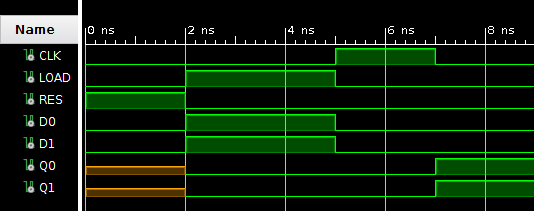
\includegraphics[width=\textwidth]{reg2_waveform.png}
    \caption[Verhalten des 2-Bit-Registers]{Zu Beginn wird das Register über
             das \texttt{res}"=Signal zurückgesetzt. Dadurch werden zunächst die
             internen Signale\texttt{q0\_s} und \texttt{q1\_s} sowie
             \SI{2}{\nano\second} später die Ausgangssignale \texttt{q0} und
             \texttt{q1} von ihrem undefinierten Zustand auf den Wert
             \glqq 0\grqq\ gesetzt. Dann wird \texttt{res} auf \glqq 0\grqq\
             gesetzt, während \texttt{load} sowie die Eingänge \texttt{d0} und
             \texttt{d1} mit \glqq 1\grqq\ belegt werden. Dadurch werden nach
             weiteren \SI{3}{\nano\second} die internen Signale \texttt{q0\_ns}
             und \texttt{q1\_ns} ebenfalls auf \glqq 1\grqq\ gesetzt. Durch das
             Anlegen der Taktflanke (\texttt{clk} = \glqq 1\grqq) nach insgesamt
             \SI{5}{\nano\second} übernehmen \texttt{q0\_s} und \texttt{q1\_s}
             die Werte von \texttt{q0\_ns} und \texttt{q1\_s}, was sich
             \SI{2}{\nano\second} später an den Ausgangssignalen zeigt.}
    \label{fpga:hdl:waveform}
\end{figure}

Der Prozess \texttt{mux} beschreibt eine kombinatorische Funktion. Er
nimmt die Signale \texttt{load}, \texttt{q0\_s}, \texttt{q1\_s},
\texttt{d0} sowie \texttt{d1} entgegen und gibt die Signale \texttt{q0\_ns} und
\texttt{q1\_ns} aus. Ist \texttt{load} logisch \glqq 1\grqq\, werden \texttt{d0}
und \texttt{d1} ausgegeben, ansonsten die gespeicherten Signale \texttt{q0\_s}
und \texttt{q1\_s}. In Moore"=Schaltwerk aus Abbildung~\ref{fpga:hdl:moore}
entspricht \texttt{mux} somit der Eingabe"=Transferfunktion.
\cite[vgl.][31]{kesel2013}

Die Ausgabe"=Transferfunktion ist in diesem Beispiel als impliziter Prozess
dargestellt: \texttt{q0} und \texttt{q1} sind die Ausgabe $Y$ des
Moore"=Schaltwerks und wurden einfach mit den internen Signalen \texttt{q0\_s}
und \texttt{q1\_s} verbunden.
\cite[vgl.][31]{kesel2013}

Prozesse sind in VHDL als Modellierungen realer Hardware zu verstehen. So lässt
sich für das oben entworfene 2"=Bit"=Register eine äquivalente
Hardware"=Schaltung aus zwei Multiplexern und zwei taktflankengesteuerten
D"=Flip"=Flops mit asynchronen Set- und Reset-Eingängen aufbauen, wie Kesel und
Bartholomä zeigen \cite[siehe][32]{kesel2013}. Die im Prozess \texttt{reg}
verwendeten Signale \texttt{q0\_s} und \texttt{q1\_s} entsprechen dabei den
Flip"=Flops, während die Multiplexer den \texttt{mux}"=Prozess implementieren.
\cite[vgl.][31]{kesel2013}


\begin{code}
    \begin{minted}[fontsize=\small]{vhdl}
ARCHITECTURE beh OF reg2 IS
    SIGNAL q0_s, q0_ns, q1_s, q1_ns : std_logic;
BEGIN
    reg: PROCESS (clk, res)
    BEGIN
        IF res = '1' THEN
            q0_s <= '0';
            q1_s <= '0';
        ELSIF clk'event AND clk = '1' THEN
            q0_s <= q0_ns;
            q1_s <= q1_ns;
        END IF;
    END PROCESS reg;

    q0 <= q0_s AFTER 2 ns;
    q1 <= q1_s AFTER 2 ns;

    mux: PROCESS (load, q0_s, q1_s, d0, d1)
    BEGIN
        IF load = '1' THEN
            q0_ns <= d0 AFTER 3 ns;
            q1_ns <= d1 AFTER 3 ns;
        ELSE
            q0_ns <= q0_s AFTER 4 ns;
            q1_ns <= q1_s AFTER 4 ns;
        END IF;
    END PROCESS mux;
END beh;
    \end{minted}
    \caption{Verhaltensbeschreibung eines 2-Bit-Registers \cite[siehe][28]{kesel2013}}
    \label{fpga:hdl:regbeh}
\end{code}

\subsubsection{Strukturbeschreibungen}

Eine Strukturbeschreibung (auch Netzliste genannt) besteht aus mehreren
Teil-Komponenten, die zu einer größeren, komplexeren Komponente 
zusammengeschaltet werden. So lässt sich für die aus den vorherigen Abschnitten
bekannte \texttt{reg2}"=\textit{Entity} aus einem Modell eines Multiplexers
sowie einem Modell eines Flip"=Flops zusammensetzen (siehe
Quelltext~\ref{fpga:hdl:regstruct}\footnote{Die Verhaltensbeschreibungen der
Komponenten \texttt{mux2} und \texttt{ff2} sind in
Anhang~\ref{anhang:source:vhdl} zu finden.}).

Wie bei der Verhaltensbeschreibung gibt es auch bei der Strukturbeschreibung
Ports, das heißt von außen ein- bzw.\ nach außen ausgehende Signale, sowie
interne Signale für die Kommunikation der Teil-Komponenten untereinander. Die
einzelnen Komponenten werden zunächst mit ihren lokalen Ports deklariert
(\texttt{COMPONENT}"=Abschnitte) und danach instanziiert; \texttt{I1} und
\texttt{I0} sind dabei Bezeichnungen für eine \textit{Instanz} der jeweiligen
\texttt{Entity}. In der \texttt{PORT MAP} werden die Ports und Signale der
Komponente den lokalen Ports der Teil-Komponenten zugeordnet.
\cite[vgl.][37]{kesel2013}

\begin{code}
    \begin{minted}[fontsize=\small]{vhdl}
ARCHITECTURE struct of reg2
    SIGNAL o1          : std_logic;
    SIGNAL o2          : std_logic;
    SIGNAL q0_internal : std_logic;
    SIGNAL q1_internal : std_logic;

    COMPONENT ff2
    PORT (
        clk : IN    std_logic;
        d0  : IN    std_logic;
        d1  : IN    std_logic;
        res : IN    std_logic;
        q0  : OUT   std_logic;
        q1  : OUT   std_logic
    );
    END COMPONENT;
    COMPONENT mux2
    PORT (
        a1  : IN    std_logic;
        a2  : IN    std_logic;
        b1  : IN    std_logic;
        b2  : IN    std_logic;
        sel : IN    std_logic;
        o1  : OUT   std_logic;
        o2  : OUT   std_logic
    );
    END COMPONENT;

BEGIN

    I1  : ff2
        PORT MAP(
            clk => clk, d0 => o1, d1 => o2,
            res => res, q0 => q0_internal, q1 => q1_internal
        );
    I0  : mux2
        PORT MAP(
            a1 => d0, a2 => d1, b1 => q0_internal,
            b2 => q1_internal, sel => load, o1 => o1, o2 => o2
        );

    q0 <= q0_internal;
    q1 <= q1_internal;

END struct;
    \end{minted}
    \caption{Strukturbeschreibung eines 2-Bit-Registers \cite[siehe][36]{kesel2013}}
    \label{fpga:hdl:regstruct}
\end{code}
\noindent

\subsubsection{Weitere Konzepte}

Die hier vorgestellten Konzepte einer Hardware"=Beschreibungssprache bilden nur
einen sehr geringen Teil der zur Verfügung stehenden Möglichkeiten ab. Neben den
gezeigten Grundbausteinen verfügen VHDL und Verilog noch über weitergehende
Fähigkeiten, wie etwa Verzweigungen, Schleifen, Operatoren und deren Überladung
oder rudimentäre Objektorientierung. Aufgrund der Zielsetzung dieser Arbeit kann
hier nicht weiter darauf eingegangen werden. Eine sehr gute Einführung in die
Programmierung mit VHDL ist aber bei Kesel und Bartholomä zu finden
\cite[siehe][]{kesel2013}. 

\subsubsection{Nebenläufigkeit}

Einer der wesentlichen Unterschiede zwischen VHDL und Hochsprachen, die auf
der algorithmischen Ebene arbeiten, ist die von vornherein vorhandene
Nebenläufigkeit. Während Befehle in C++ nacheinander abgearbeitet werden, gilt
dies bei VHDL nur innerhalb eines \textit{Prozesses}. \textit{Prozesse} arbeiten
unabhängig voneinander und werden nur über ihre Eingangssignale gesteuert, was
sich so auch auf die reale Hardware abbilden lässt. \cite[vgl.][25]{kesel2013}

\subsection{High-Level-Synthese und Parallelität}\label{fpga:entwicklung:hls}

Aus den im vorherigen Abschnitt gezeigten Beispielen wird schnell ersichtlich,
dass der Entwurf komplexerer Schaltungen mit einem hohen Konzeptions- und
Arbeitsaufwand verbunden ist und nicht nur gute Kenntnisse des  abzubildenden
Algorithmus erfordert, sondern darüber hinaus auch Wissen über die
Digitaltechnik verlangt. Mit der High"=Level"=Synthese (HLS) gibt es einen
Ansatz, die konkrete Schaltung durch Abstraktion zu verbergen und sich dem
Programmiermodell anderer Hardware"=Typen (\gls{cpu}s, \gls{gpu}s) anzunähern.
Bei der HLS findet der Entwurf vollständig auf der algorithmischen oder
Systemebene statt. Anschließend wird aus dem erzeugten Modell durch
HLS"=Werkzeuge ein Modell auf der Register"=Transfer"=Ebene erzeugt, aus dem im
nächsten Schritt die konkrete Schaltung synthetisiert werden kann. Auf
herkömmliche Programmiersprachen übertragen entspricht der Entwurf mit einer
Hardware"=Beschreibungssprache also der Programmierung einer \gls{cpu} mit einer
Assemblersprache.
\cite[vgl.][7]{hlsintro2019}

Während des algorithmischen Entwurfs kann der Nutzer zudem Randbedingungen
festlegen, die die HLS steuern, wie z.B. den angestrebten Ressourcenbedarf,
den gewünschten Datendurchsatz, \textit{Pipelining} oder die
Konfiguration des BlockRAMs. Bei der Erzeugung des Register"=Transfer"=Modells
werden diese Randbedingungen dann von den HLS"=Werkzeugen berücksichtigt.
\cite[vgl.][482]{kesel2013}

Die HLS wird zur Zeit von einigen Herstellern für mehrere Programmiersprachen
bzw. Erweiterungen bestehender Programmiersprachen unterstützt. Der Hersteller
Xilinx bietet beispielsweise HLS"=Werkzeuge für die Sprachen C, C++ und SystemC
an und unterstützt darüber hinaus den \gls{opencl}"=Standard. Einen ähnlichen
Weg geht die Firma Intel, die HLS"=Werkzeuge für C und C++ sowie \gls{opencl}
anbietet.

Die folgenden Erläuterungen richten sich nach den Handbüchern des Herstellers
Xilinx, die zugrunde liegenden Konzepte gelten jedoch für alle \gls{fpga}s.

\subsubsection{Scheduling}

\gls{fpga}s sind inhärent parallel. Anweisungen, die von einem bestimmten
Hardware"=Abschnitt ausgeführt werden (in VHDL durch \textit{Prozesse}
modelliert), sind sequentiell, während unterschiedliche Hardware"=Abschnitte in
Bezug aufeinander nebenläufig sind. Diese Eigenschaft unterscheidet \gls{fpga}s
deutlich von Prozessorarchitekturen, wie das folgende Beispiel zeigt.

Jeder Prozessor führt ein Programm als eine Folge von Instruktionen aus. Diese
Instruktionen werden von Compilern aus einer Hochsprache wie C++ in eine
prozessorspezifische Assemblersprache übersetzt:
\begin{code}
    \begin{minted}[fontsize=\small]{c++}
z = a + b;
    \end{minted}
\end{code}
wird wie folgt transformiert:
\begin{code}
    \begin{minted}[fontsize=\small]{gas}
movl    -8(%rbp), %edx
movl    -4(%rbp), %edx
addl    %edx, %eax
movl    %eax, -12(%rbp)
    \end{minted}
\end{code}
Selbst eine relativ simple Operation wie die Addition zweier Zahlen resultiert
in vier sequentiell auszuführenden Maschineninstruktionen. Je nachdem, wo die
Operanden liegen oder wo das Ergebnis gespeichert werden soll, können die
Instruktionen für Laden und Speichern (im Verhältnis zur Addition) viele
Taktzyklen benötigen. \cite[vgl.][18]{hlsintro2019}

Soll die Addition für viele Elemente ausgeführt werden, wie zum Beispiel in
einer Schleife, müssen diese vier Instruktionen stets wiederholt werden, da sich
alle Operationen dieselbe \gls{alu} teilen.

Bei der HLS kann diese Operation auf Hardware abgebildet werden, die
ausschließlich für diese Operation verwendet wird. Wenn \texttt{a}, \texttt{b}
und \texttt{z} \SI{32}{\bit} groß sind, wird dieser Datentyp durch 32 \gls{lut}
implementiert\footnote{Eine LUT entspricht einer Wahrheitstabelle für ein Bit.}.
Im Gegensatz zu Prozessoren werden bei einer \gls{fpga}"=Implementierung für
jede Operation innerhalb des Algorithmus voneinander unabhängige
\gls{lut}"=Mengen instanziiert.
\cite[vgl.][19]{hlsintro2019}

Eine Schleife ließe sich auf \gls{fpga}s also ganz oder teilweise ausrollen und,
sofern zwischen den einzelnen Iterationen keine Abhängigkeiten bestehen,
parallel ausführen. Die während der HLS vorgenommene Analyse der Daten- und
Kontrollflussabhängigkeiten wird im \gls{fpga}"=Kontext als Scheduling
bezeichnet. \cite[vgl.][19]{hlsintro2019}

\subsubsection{Pipelining-Prinzip}

Das von Prozessoren bekannte Prinzip des \textit{Pipelinings} findet bei
\gls{fpga}s ebenfalls Anwendung. Dabei werden Datenabhängigkeiten so aufgeteilt,
dass die ursprüngliche Verarbeitungsreihenfolge beibehalten wird, während die
benötigten Hardware"=Einheiten in eine Verkettung unabhängiger Stufen unterteilt
werden. Jede Stufe erhält ihre Eingangsdaten von der vorherigen Stufe und reicht
ihr Teilergebnis an die nächste Stufe weiter. Beispielsweise lässt sich die
folgende Funktion auf einen Multiplizierer und zwei Addierer abbilden:
\[
    y = (a \cdot x) + b + c
\]
Die resultierende Hardware"=Schaltung ist in
Abbildung~\ref{fpga:pipelining:schaltung} dargestellt. Die obere Schaltung
berechnet $y$ ohne Pipelining, die untere Schaltung zeigt die transformierte
Schaltung mit Pipelining.
\begin{figure}[htb]
    \centering
    \begin{tikzpicture}
        % untere Schaltung
        % a
        \draw (0.2, 5.15) -- (0.4, 5.35) node [pos = 1.0, xshift = 1.2mm, yshift = 2mm] {$a$};
        \draw (0, 5.25) -- (0.75, 5.25);
        \draw [thick, fill = HKS92!50] (0.75, 5) rectangle (1.25, 5.5);
        \draw [-{Latex}] (1.25, 5.25) -- (2.25, 5.25) -- (2.25, 4.75);

        % x
        \draw (0.2, 2.65) -- (0.4, 2.85) node [pos = 1.0, xshift = 1.2mm, yshift = 2mm] {$x$};
        \draw (0, 2.75) -- (0.75, 2.75);
        \draw [thick, fill = HKS92!50] (0.75, 2.5) rectangle (1.25, 3);
        \draw [-{Latex}] (1.25, 2.75) -- (2.25, 2.75) -- (2.25, 3.25);

        % b
        \draw (0.2, 1.4) -- (0.4, 1.6) node [pos = 1.0, xshift = 1.2mm, yshift = 2mm] {$b$};
        \draw (0, 1.5) -- (0.75, 1.5);
        \draw [thick, fill = HKS92!50] (0.75, 1.25) rectangle (1.25, 1.75);
        \draw (1.25, 1.5) -- (3.5, 1.5);
        \draw [thick, fill = HKS92!50] (3.5, 1.25)  rectangle (4, 1.75);
        \draw [-{Latex}] (4, 1.5) -- (6, 1.5) -- (6, 2);

        % c
        \draw (0.2, 0.15) -- (0.4, 0.35) node [pos = 1.0, xshift = 1.2mm, yshift = 2mm] {$c$};
        \draw (0, 0.25) -- (0.75, 0.25);
        \draw [thick, fill = HKS92!50] (0.75, 0) rectangle (1.25, 0.5);
        \draw (1.25, 0.25) -- (3.5, 0.25);
        \draw [thick, fill = HKS92!50] (3.5, 0) rectangle (4, 0.5);
        \draw [-{Latex}] (4, 0.25) -- (8.75, 0.25) -- (8.75, 0.75);

        % Multiplizierer
        \draw [thick] (2.25, 4) circle [radius = 0.75] node {\textbf{*}};
        \draw (3.0, 4) -- (3.5, 4);
        \draw [thick, fill = HKS92!50] (3.5, 3.75) rectangle (4, 4.25);
        \draw [-{Latex}] (4, 4) -- (6, 4) -- (6, 3.5);

        % erster Addierer
        \draw [thick] (6, 2.75) circle [radius = 0.75] node {\textbf{+}};
        \draw [-{Latex}] (6.75, 2.75) -- (8.75, 2.75) -- (8.75, 2.25);

        % zweiter Addierer
        \draw [thick] (8.75, 1.5) circle [radius = 0.75] node {\textbf{+}}; 

        % y
        \draw (9.5, 1.5) -- (10.25, 1.5);
        \draw [thick, fill = HKS92!50] (10.25, 1.25) rectangle (10.75, 1.75);
        \draw [-{Latex}] (10.75, 1.5) -- (11.5, 1.5);
        \draw (11.0, 1.4) -- (11.2, 1.6) node [pos = 1.0, xshift = 1.2mm, yshift = 2mm] {$y$};

        % Pfeil
        \draw (6, 5.75) -- ++(135:0.71) 
                        -- ++(0.25,0) 
                        -- ++(0, 0.75) 
                        -- ++(0.5, 0) 
                        -- ++(0, -0.75) node [right, xshift = 3mm] {\small Pipeline-Transformation}
                        -- ++(0.25, 0) 
                        -- ++(-135:0.71);

        % obere Schaltung
        % a
        \draw (0.2, 12.65) -- (0.4, 12.85) node [pos = 1.0, xshift = 1.2mm, yshift = 2mm] {$a$};
        \draw [-{Latex}] (0, 12.75) -- (2.25, 12.75) -- (2.25, 12.25);

        % x
        \draw (0.2, 10.15) -- (0.4, 10.35) node [pos = 1.0, xshift = 1.2mm, yshift = 2mm] {$x$};
        \draw [-{Latex}] (0, 10.25) -- (2.25, 10.25) -- (2.25, 10.75);

        % b
        \draw (0.2, 8.9) -- (0.4, 9.1) node [pos = 1.0, xshift = 1.2mm, yshift = 2mm] {$b$};
        \draw [-{Latex}] (0, 9) -- (6, 9) -- (6, 9.5);

        % c
        \draw (0.2, 7.65) -- (0.4, 7.85) node [pos = 1.0, xshift = 1.2mm, yshift = 2mm] {$c$};
        \draw [-{Latex}] (0, 7.75) -- (8.75, 7.75) -- (8.75, 8.25);

        % Multiplizierer
        \draw [thick] (2.25, 11.5) circle [radius = 0.75] node {\textbf{*}};
        \draw [-{Latex}] (3, 11.5) -- (6, 11.5) -- (6, 11);

        % erster Addierer
        \draw [thick] (6, 10.25) circle [radius = 0.75] node {\textbf{+}};
        \draw [-{Latex}] (6.75, 10.25) -- (8.75, 10.25) -- (8.75, 9.75);

        % zweiter Addierer
        \draw [thick] (8.75, 9) circle [radius = 0.75] node {\textbf{+}}; 

        % y
        \draw [-{Latex}] (9.5, 9) -- (11.5, 9);
        \draw (11.0, 8.9) -- (11.2, 9.1) node [pos = 1.0, xshift = 1.2mm, yshift = 2mm] {$y$};
    \end{tikzpicture}
    \caption{FPGA"=Implementierung einer mehrstufigen Berechnung \cite[nach][21]{hlsintro2019}}
    \label{fpga:pipelining:schaltung}
\end{figure}
\noindent
Die grauen Kästen der unteren Schaltung entsprechen Registern, die in realer
Hardware durch Flip"=Flops realisiert werden. Jeder Kasten kann dabei als ein
zusätzlicher Taktzyklus aufgefasst werden. Die Berechnung eines einzelnen
Ergebnisses benötigt dadurch drei zusätzliche Taktzyklen. Durch die zusätzlichen
Register lassen sich die einzelnen Schritte der Berechnung jedoch in unabhängige
Abschnitte aufteilen, der Multiplizierer und die Addierer können also
nebenläufig arbeiten. Die Ergebnisse $y$ und $y'$ lassen sich auf diese Weise
(teilweise) parallel berechnen und lasten dabei die verfügbare Hardware besser
aus: nach einem Overhead von 3 Taktzyklen zu Beginn der Berechnung (engl.
\textit{pipeline fill time}) berechnet die Schaltung in jedem weiteren
Taktzyklus einen neuen Wert für $y$. Dieser Vorgang wird in
Abbildung~\ref{fpga:pipelining:pipeline} illustriert. Je nach verwendetem
Algorithmus ist es möglich, dass die Pipeline nicht in jedem Taktzyklus eine
neue Schleifeniteration verarbeiten kann (z.B. aufgrund bestehender
Abhängigkeiten zwischen einzelnen Iterationen). Die Anzahl der Zyklen, die
zwischen dem Beginn zweier aufeinanderfolgender Iterationen liegen, werden als
\gls{ii} bezeichnet. Wenn $\text{II} = 1$ gilt, beginnt die Pipeline mit
jedem Takt eine neue Schleifeniteration. Bei $\text{II} = 2$ kann sie dies nur
alle zwei Takte tun, bei $\text{II} = 4$ mit jedem vierten Takt, usw.
\cite[vgl.][20--21]{hlsintro2019}

\begin{figure}[htb]
    \centering
    \begin{tikzpicture}
        % a
        \draw (0.2, 5.15) -- (0.4, 5.35) node [pos = 1.0, xshift = 1.2mm, yshift = 2mm] {$a$};
        \draw (0, 5.25) -- (0.75, 5.25);
        \draw [thick, fill = HKS92!75] (0.75, 5) rectangle (1.25, 5.5);
        \draw [-{Latex}] (1.25, 5.25) -- (2.25, 5.25) -- (2.25, 4.75);

        % x
        \draw (0.2, 2.65) -- (0.4, 2.85) node [pos = 1.0, xshift = 1.2mm, yshift = 2mm] {$x$};
        \draw (0, 2.75) -- (0.75, 2.75);
        \draw [thick, fill = HKS92!75] (0.75, 2.5) rectangle (1.25, 3);
        \draw [-{Latex}] (1.25, 2.75) -- (2.25, 2.75) -- (2.25, 3.25);

        % b
        \draw (0.2, 1.4) -- (0.4, 1.6) node [pos = 1.0, xshift = 1.2mm, yshift = 2mm] {$b$};
        \draw (0, 1.5) -- (0.75, 1.5);
        \draw [thick, fill = HKS92!75] (0.75, 1.25) rectangle (1.25, 1.75);
        \draw (1.25, 1.5) -- (3.5, 1.5);
        \draw [thick] (3.5, 1.25) rectangle (4, 1.75);
        \draw [-{Latex}] (4, 1.5) -- (6, 1.5) -- (6, 2);

        % c
        \draw (0.2, 0.15) -- (0.4, 0.35) node [pos = 1.0, xshift = 1.2mm, yshift = 2mm] {$c$};
        \draw (0, 0.25) -- (0.75, 0.25);
        \draw [thick, fill = HKS92!75] (0.75, 0) rectangle (1.25, 0.5);
        \draw (1.25, 0.25) -- (3.5, 0.25);
        \draw [thick] (3.5, 0) rectangle (4, 0.5);
        \draw [-{Latex}] (4, 0.25) -- (8.75, 0.25) -- (8.75, 0.75);

        % Multiplizierer
        \draw [thick] (2.25, 4) circle [radius = 0.75] node {\textbf{*}};
        \draw (3.0, 4) -- (3.5, 4);
        \draw [thick] (3.5, 3.75) rectangle (4, 4.25);
        \draw [-{Latex}] (4, 4) -- (6, 4) -- (6, 3.5);

        % erster Addierer
        \draw [thick, fill = HKS92!50] (6, 2.75) circle [radius = 0.75] node {\textbf{+}};
        \draw [-{Latex}] (6.75, 2.75) -- (8.75, 2.75) -- (8.75, 2.25);

        % zweiter Addierer
        \draw [thick, fill = HKS92!50] (8.75, 1.5) circle [radius = 0.75] node {\textbf{+}}; 

        % y
        \draw (9.5, 1.5) -- (10.25, 1.5);
        \draw [thick, fill = HKS92!50] (10.25, 1.25) rectangle (10.75, 1.75);
        \draw [-{Latex}] (10.75, 1.5) -- (11.5, 1.5);
        \draw (11.0, 1.4) -- (11.2, 1.6) node [pos = 1.0, xshift = 1.2mm, yshift = 2mm] {$y$};

        % Formeln
        \draw [thick, fill = HKS92!75] (-1, -3.5) rectangle (1.35, -0.5)
              node [pos = 0.5, align = center, text = white] { $a(i)$ \\ 
                                                               $x(i)$ \\ 
                                                               $b(i)$ \\ 
                                                               $c(i)$ };
        \draw [thick] (1.35, -3.5) rectangle (4.5, -0.5)
              node [pos = 0.5, align = center] { $a(i - 1) \cdot x(i - 1)$ \\
                                                 $b(i - 1)$ \\
                                                 $c(i - 1)$};
        \draw [thick, fill = HKS92!50] (4.5, -3.5) rectangle (11.5, -0.5)
              node [pos = 0.5, align = center] { $(a(i - 2) \cdot x(i - 2)) + b(i - 2) + c(i - 2)$};
    \end{tikzpicture}
    \caption{FPGA"=Pipeline"=Architektur \cite[nach][22]{hlsintro2019}}
    \label{fpga:pipelining:pipeline}
\end{figure}

Die Anwendung des Pipelining während der HLS unterscheidet sich zwischen den
Herstellern: so versucht Intels OpenCL"=Umgebung grundsätzlich, Pipelining auf
jede vorhandene Schleife anzuwenden und erfordert ein explizites Deaktivieren
des Verfahrens, wenn kein Pipelining gewünscht wird. Bei Xilinx'
OpenCL"=Umgebung verhält es sich dagegen genau umgekehrt, da hier Pipelining
explizit angeschaltet werden muss.

\subsubsection{Producer-Consumer-Prinzip}

Neben dem Pipelining gibt es auf \gls{fpga}s eine weitere Möglichkeit,
Parallelität auszudrücken. Diese ähnelt dem Pipelining-Prinzip, arbeitet jedoch
auf einer groberen Ebene. Dahinter steht das Ziel, diese Funktionen
weitestgehend parallel auszuführen. Dazu analysieren die HLS"=Werkzeuge die Ein- 
und Ausgangsparameter der im Algorithmus vorhandenen Funktionen. Im einfachsten
Fall gibt es keine gemeinsam bearbeiteten Daten, wodurch alle Funktionen
parallel ausgeführt werden können. Naturgemäß ist dieser Fall recht selten,
üblicherweise werden die Ergebnisse einer Funktion von einer oder mehreren
nachfolgenden Funktionen verarbeitet. Dieses als
\textit{Producer"=Consumer}"=Prinzip bekannte Verfahren kann durch die
Nebenläufigkeit der FPGA"=Hardware parallelisiert werden. Durch den Einsatz von
Block RAM als FIFO"=Puffer zwischen den Hardware"=Abschnitten, die aus der
jeweiligen Funktion synthetisiert wurden, kann die produzierende Funktion
während ihrer Ausführung Teilergebnisse speichern. Die konsumierende Funktion
kann diese Teilergebnisse nach der initialen Wartezeit, die ebenfalls als
\gls{ii} bezeichnet wird, direkt weiter verarbeiten, ohne auf das Ende der
produzierenden Funktion bzw.\ das resultierende Gesamtergebnis warten zu müssen.
\cite[vgl.][22--23]{hlsintro2019}

Das Producer"=Consumer"=Prinzip wird je nach Hersteller unterschiedlich benannt.
So nennt sich dieses Verfahren bei Xilinx \textit{Dataflow}, während es bei
Intel \textit{Channel} heißt.

\chapter{Der SYCL-Standard}\label{sycl}

Durch die Xilinx"=Implementierung der vor einigen Jahren veröffentlichten
SYCL"=Spezifikation gibt es eine weitere Möglichkeit, ein Problem auf
algorithmischer Ebene zu beschreiben und über die HLS in eine
\gls{fpga}"=Schaltung zu synthetisieren. Eine einfache SYCL"=Einführung sowie
die für \gls{fpga}s wichtigen Besonderheiten sind daher das Thema dieses
Kapitels.

\section{Überblick}\label{sycl:ueberblick}

Mit dem SYCL"=Standard\footnote{Entgegen des optischen Anscheins ist
\glqq SYCL\grqq\ kein Akronym, sondern ein Eigenname.}\cite[vgl.][]{sycl2019}
verfolgt die herausgebende Khronos"=Gruppe das Ziel eines abstrakten
C++"=Programmiermodells für \gls{opencl}, das die Flexibilität und Einfachheit
moderner C++"=Standards bieten soll, während gleichzeitig Konzeption und
Portabilität des \gls{opencl}"=1.2"=Standards \cite[vgl.][]{opencl2012}
beibehalten werden.

Von \gls{opencl} erbt SYCL damit den Anspruch, eine einheitliche
Programmierschnittstelle für verschiedene Beschleunigertypen unterschiedlicher
Hersteller zu bieten. Das heißt, dass ein einmal geschriebener Quelltext, der
auf einem Beschleuniger ausgeführt werden soll, möglichst ohne große Änderungen
sowohl auf einer \gls{cpu}, einer \gls{gpu}, einem \gls{dsp} oder einem
\gls{fpga} ausführbar sein soll.

SYCL unterscheidet sich von \gls{opencl} im Hinblick auf die Struktur des
Quelltextes: Bei \gls{opencl} sind die Quelltexte für das steuernde Programm
(\textit{Host}) und den Programmteil, der vom Beschleuniger (\textit{Device})
ausgeführt wird, voneinander getrennt. Diese Design"=Entscheidung des
\gls{opencl}"=Standards ist durch das Ziel der Plattformunabhängigkeit
begründet: Ein Entwickler kennt während der Kompilierung des Hauptprogramms
nicht notwendigerweise die vorhandenen Beschleuniger der Zielplattform. Dadurch
wird der \textit{Device}"=spezifische Quelltext häufig erst zur Laufzeit des
Programms kompiliert, da in diesem Moment der konkrete Beschleuniger bekannt
ist. Dieser Ansatz hat jedoch den Nachteil, dass der Compiler des
\textit{Device}"=Quelltexts (im Folgenden als \textit{Kernel} bezeichnet) keine
Annahmen über das \textit{Host}"=Programm bzw. den den \textit{Kernel}
umgebenden Quelltext mehr treffen kann, was zu einem geringeren
Optimierungspotential führt. \gls{opencl}"=\textit{Kernel} lassen sich zwar auch
vor der Laufzeit des Programms für eine konkrete Zielplattform kompilieren (dies
geschieht aufgrund der langen Kompilierungszeiten bei \gls{fpga}s), büßen
dadurch aber ihre Plattformunabhängigkeit ein.

Ein SYCL-Quelltext kennt dagegen keine strikte Trennung zwischen \textit{Host}-
und \textit{Device}"=Anweisungen, was zu einer besseren Analyse des den
\textit{Kernel} umgebenden Kontexts führt. Außerdem ergibt sich der weitere
Vorteil, dass \textit{Host} und \textit{Device} Quelltext teilen können, wie
z.B.\ beidseitig verwendete Hilfsfunktionen. Der \textit{Kernel} wird dabei vom
\textit{Device}"=Compiler extrahiert und in eine Form umgewandelt, die von der
Ziel"=Hardware zur Laufzeit kompiliert oder ausgeführt werden kann.
\cite[vgl][35]{sycl2019}

Ein weiterer wichtiger Unterschied zu \gls{opencl} besteht darin, dass
jedes SYCL"=Programm mit einem Standard"=C++"=Compiler übersetzt werden kann,
sofern keine direkten Interaktionen mit \gls{opencl} selbst erfolgen. Damit
lässt sich ein SYCL"=Programm auf jeder \gls{cpu} ausführen, für die ein
(moderner) C++"=Compiler existiert, wenngleich dies Einschränkungen bei der
erreichbaren Leistung bedeuten kann. So schreibt die SYCL"=Spezifikation für
diesen Fall nur die Ausführbarkeit selbst vor, aber nicht die Nutzung aller
\gls{cpu}"=Kerne oder Vektorregister. \cite[vgl.][15]{sycl2019}

Seit der ersten Veröffentlichung im März 2014 \cite[vgl.][]{khronos2014} mit der
Versionsnummer 1.2 wurde die SYCL"=Spezifikation stetig weiterentwickelt; die
zur Zeit aktuelle Spezifikation vom April 2019 trägt die Revisionsnummer 1.2.1
Revision 5. \cite[vgl.][1]{sycl2019}

Teil der Khronos"=Gruppe sind (unter anderen) die \gls{fpga}"=Hersteller Xilinx
und Intel. Xilinx unterstützt den SYCL"=Standard in Form einer Erweiterung der
bestehenden HLS"=Werkzeuge bereits, während Intel dies für die eigenen FPGAs
mittelfristig plant; für Intel"=\gls{cpu}s und "=\gls{gpu}s ist bereits eine
SYCL"=Implementierung verfügbar (der Abschnitt~\ref{sycl:implementierungen}
befasst sich mit allen verfügbaren Implementierungen).

\subsection{Der AXPY-Algorithmus als Beispiel}
\label{sycl:ueberblick:axpy}

Ein im Bereich der parallelen Programmierung häufig verwendetes einführendes
Beispiel ist der sogenannte AXPY"=Algorithmus, der ursprünglich aus der
Bibliothek \textit{Basic Linear Algebra Subprograms} (\gls{blas}) stammt
\cite[vgl.][]{lawson1979}. Dieser führt die Berechnung

\begin{equation}\label{sycl:ueberblick:axpy:formel}
    \vec{y} = a \cdot \vec{x} + \vec{y}
\end{equation}

aus und ist aufgrund seiner Einfachheit und hohen erreichbaren Parallelität
(sofern $\vec{x}$ und $\vec{y}$ viele Elemente enthalten) sehr beliebt.

AXPY lässt sich für eine Einführung in SYCL gut verwenden und wird daher in den
folgenden Abschnitten als illustrierendes Beispiel genutzt.

\subsection{Struktur eines SYCL-Programms}

Ein SYCL"=Programm lässt sich in mehrere aufeinander aufbauende Stufen
unterteilen, wie in Quelltext~\ref{sycl:ueberblick:axpy:struktur} zu sehen ist.
Die einzelnen Platzhalter im Quelltext werden in den nächsten Abschnitten mit
Inhalt gefüllt.

\begin{code}
    \begin{minted}[fontsize=\small]{c++}
#include <cstdlib>
#include <CL/sycl.hpp>

auto main() -> int
{
    // Beschleunigerwahl und Befehlswarteschlange

    // Speicherreservierung und -initialisierung

    // Kernel-Definition und -ausführung

    // Synchronisierung

    return EXIT_SUCCESS;
}
    \end{minted}
    \caption{Struktur eines SYCL-Programms}
    \label{sycl:ueberblick:axpy:struktur}
\end{code}

\subsection{Beschleunigerwahl und Befehlswarteschlange}
\label{sycl:ueberblick:axpy:queue}

Von \gls{opencl} erbt SYCL die Plattformunabhängigkeit. Es wird das
Vorhandensein mindestens einer \gls{opencl}"=Plattform auf dem System
angenommen\footnote{Diese wird aber nicht vorausgesetzt! Jede
SYCL"=Implementierung muss auch ohne eine OpenCL"=Plattform auf dem Host
lauffähig sein.}, was im Umkehrschluss bedeutet, dass unter Umständen zwischen
mehreren verschiedenen Plattformen konkurrierender Hersteller gewählt werden
muss. 

Die SYCL"=Spezifikation bietet dem Programmierer mehrere Möglichkeiten, die
gewünschte Plattform für sein Programm auszuwählen. Der einfachste Ansatz
besteht darin, eine Befehlswarteschlange (die \textit{Queue} genannt wird) für
einen Beschleuniger zu konstruieren. Über die \textit{Queue} erfolgt die
Kommunikation zwischen dem \textit{Host} und einem \textit{Device}, also
Kopieroperationen, das Starten eines \textit{Kernels} sowie die
Synchronisierung. Letztere ist notwendig, da es sich bei dem \textit{Device}
um eine vom \textit{Host} weitestgehend unabhängige Hardware handelt, die
Operationen also (aus Sicht des \textit{Hosts}) asynchron ablaufen.

Jedes genutzte \textit{Device} erhält in SYCL mindestens eine eigene
\textit{Queue}, so dass auch die Nutzung mehrerer Beschleuniger möglich ist.

Eine \textit{Queue} kann durch das Übergeben eines Auswahlkriteriums für das
gewünschte \textit{Device} konstruiert werden. Die Auswahlkriterien werden in
der SYCL"=Spezifikation \texttt{device\_selector} genannt. Neben den in der
Spezifikation vorhandenen Kriterien (beispielsweise \texttt{cpu\_selector},
\texttt{gpu\_selector} oder \texttt{host\_selector}) ist es Herstellern oder
Programmierern selbst möglich, durch das Erben von der Elternklasse
\texttt{device\_selector} eigene Kriterien zu definieren. Beispielsweise findet
sich in den Testfällen der von Xilinx entwickelten SYCL"=Implementierung ein
\texttt{device\_selector} für die eigenen Geräte, der die \gls{fpga}s über den
Firmennamen findet. Mit dessen Hilfe lässt sich die \textit{Queue} für ein
Xilinx"=FPGA wie in Quelltext~\ref{sycl:ueberblick:axpy:queue:src} dargestellt
erzeugen.
%
\begin{code}
    \begin{minted}[fontsize=\small]{c++}
class XOCLDeviceSelector : public cl::sycl::device_selector {
    public:
        int operator()(const cl::sycl::device &Device) const override {
            const std::string DeviceVendor =
                            Device.get_info<cl::sycl::info::device::vendor>();
            return (DeviceVendor.find("Xilinx") != std::string::npos) ? 1 : -1;
        }
};

/* ... */

auto queue = cl::sycl::queue{XOCLDeviceSelector{}};
    \end{minted}
    \caption{Auswahl eines Xilinx"=FPGAs und Erzeugung einer zugehörigen
             \textit{Queue}}
    \label{sycl:ueberblick:axpy:queue:src}
\end{code}
%
\vspace{5mm}
Programmierern, die mehr Kontrolle über die Initialisierung des Beschleunigers
oder der gesamten SYCL"=Laufzeitumgebung wünschen, stellt die
SYCL"=Spezifikation das aus \gls{opencl} bekannte Schema zur Verfügung. Der
Programmierer kann zunächst eine Liste aller zur Verfügung stehenden
\gls{opencl}"=Plattformen anfordern, aus denen er frei wählen kann. Auf dem
Fundament der gewählten Plattform erzeugt der Programmierer im nächsten Schritt
einen SYCL"=Kontext (der einen \gls{opencl}"=Kontext kapselt). Der Kontext
stellt wiederum eine Liste aller \textit{Devices} der Plattform bereit, aus der
ein oder mehrere Beschleuniger ausgesucht werden können. Die Auswahl dient dann
als Parameter für die Erzeugung einer SYCL"=\textit{Queue}. In jedem der
genannten Schritte stehen dem Programmierer zahlreiche Informationen über die
jeweilige Klasse zur Verfügung (Hersteller der Plattform oder des
Beschleunigers, Hardware"=Eigenschaften, verfügbare Erweiterungen, usw.), die
eine Verfeinerung der Auswahl erlauben.

Der Quelltext~\ref{sycl:ueberblick:axpy:queue:ausfuehrlich} zeigt das
ausführliche Schema. In den folgenden Abschnitten wird jedoch die oben gezeigte,
einfachere und kürzere Variante verwendet.

\begin{code}
    \begin{minted}[fontsize=\small]{c++}
auto platforms = cl::sycl::platform::get_platforms();
auto my_platform = /* ... */;

auto context = cl::sycl::context{my_platform};

auto devices = context.get_devices();
auto my_device = /* ... */;

auto queue = cl::sycl::queue{my_device};
    \end{minted}
    \caption{Ausführliche Beschleunigerwahl und \textit{Queue}"=Konstruktion}
    \label{sycl:ueberblick:axpy:queue:ausfuehrlich}
\end{code}

\subsection{Speicherreservierung und -initialisierung}
\label{sycl:ueberblick:axpy:buffer}

Für die Vektoren $\vec{x}$ und $\vec{y}$ der
Formel~\ref{sycl:ueberblick:axpy:formel} ist eine Speicherreservierung auf dem
\textit{Device} sowie die Initialisierung des reservierten Speichers notwendig
(die Konstante $a$ kann als einfacher Parameter übergeben werden). SYCL stellt
dafür zwei Klassen bereit:
%
\begin{itemize}
    \item Ein \texttt{buffer} kapselt die auf dem \textit{Device} reservierten
          Speicherbereiche. Dabei ist zu beachten, dass ein \texttt{buffer}
          keinem \textit{Device} direkt zugeordnet ist, sondern dem gesamten
          Kontext zur Verfügung steht. Ein \texttt{buffer} kann so auch auf
          mehreren \textit{Devices} verwendet werden. Die notwendige
          Synchronisierung wird von der SYCL"=Laufzeitumgebung vorgenommen.
    \item Ein \texttt{accessor} sorgt für den Zugriff auf den von einem
          \texttt{buffer} verwalteten Speicher. Es existieren verschiedene
          \texttt{accessor}"=Typen, darunter auch einer für den Speicherzugriff
          auf der \textit{Host}"=Seite. Mit diesem lässt sich ein
          \texttt{buffer} direkt initialisieren, ohne eine explizite Kopie
          anstoßen zu müssen. Aus Sicht des Programmierers lässt sich ein
          \texttt{accessor} wie ein Zeiger oder Feld verwenden, d.h. über den
          \texttt{[]}"=Operator.
\end{itemize}
%
\noindent
Ein \texttt{buffer} besteht aus einer endlichen Anzahl von Elementen desselben
Typs und kann ein-, zwei- oder dreidimensional sein. Der Elemente-Typ sowie die
Dimension des Puffers sind als Template"=Parameter zur Compile"=Zeit anzugeben,
während die Anzahl als Laufzeit"=Parameter übergeben wird. Ein \texttt{accessor}
lässt sich über die Methode \texttt{get\_access} der \texttt{buffer}"=Klasse
erzeugen. Dabei wird als Template"=Parameter der gewünschte Zugriffstyp
angegeben. Diese Information wird von der SYCL"=Laufzeitumgebung zur Sortierung
der Abhängigkeiten zwischen Operationen auf dem \textit{Device} genutzt (siehe
auch Abschnitt~\ref{sycl:konzepte:abhaengigkeiten}).

SYCL unterscheidet sechs verschiedene Zugriffstypen:
\begin{itemize}
    \item \texttt{read} gestattet ausschließlich lesenden Zugriff auf den
          Puffer.
    \item \texttt{write} ermöglicht ausschließlich schreibenden Zugriff.
    \item Durch \texttt{read\_write} kann sowohl lesend als auch schreibend
          auf den \texttt{buffer} zugegriffen werden.
    \item \texttt{discard\_write} ermöglicht ausschließlich schreibenden Zugriff
          und verwirft alle vorher im Puffer enthaltenen Elemente (also auch bei
          partiellem Zugriff).
    \item \texttt{discard\_read\_write} ist die Kombination aus
          \texttt{read\_write} und \texttt{discard\_write}.
    \item \texttt{atomic} ermöglicht atomaren Zugriff bei paralleler Nutzung des
          Puffers.
\end{itemize}

Für das AXPY"=Beispiel lassen sich die benötigten Felder -- wie in
Quelltext~\ref{sycl:ueberblick:axpy:buffer:src} dargestellt -- anlegen und
initialisieren.
%
\begin{code}
    \begin{minted}[fontsize=\small]{c++}
// Puffer enthalten 1024 Elemente
const auto buf_range = cl::sycl::range<1>{1024};

// erzeuge eindimensionale Puffer für int-Elemente
auto buf_x = cl::sycl::buffer<int, 1>{buf_range};
auto buf_y = cl::sycl::buffer<int, 1>{buf_range};

// greife auf x und y zu, verwirf vorherige Elemente
auto h_acc_x = buf_x.get_access<cl::sycl::access::mode::discard_write>();
auto h_acc_y = buf_x.get_access<cl::sycl::access::mode::discard_write>();

// initialisiere x und y
for(auto i = 0; i < 1024; ++i)
{
    h_acc_x[i] = /* ... */;
    h_acc_y[i] = /* ... */;
}
    \end{minted}
    \caption{Speicherreservierung und -initialisierung in SYCL}
    \label{sycl:ueberblick:axpy:buffer:src}
\end{code}

\subsection{\textit{Kernel}-Definition und -ausführung}
\label{sycl:ueberblick:axpy:kernel}

Im nächsten Schritt wird der eigentliche \textit{Kernel} definiert und
ausgeführt. Ein SYCL"=\textit{Kernel} besteht aus zwei Teilen: Der eigentlichen
\textit{Kernel}"=Funktion, also der Abbildung des Algorithmus auf
SYCL"=C++"=Quelltext, sowie den Abhängigkeiten (in Form von
\texttt{accessor}"=Variablen). \textit{Kernel}"=Funktion und Abhängigkeiten
bilden gemeinsam eine \textit{command group} und werden in dieser Form an die
\textit{Queue} zur Ausführung übergeben. Dabei kann jede \textit{command group}
nur genau eine \textit{Kernel}"=Funktion (oder explizite Kopieroperation)
enthalten. Es bildet sich damit für das AXPY"=Beispiel das in
Quelltext~\ref{sycl:ueberblick:axpy:kernel:cg} gezeigte Grundgerüst einer
\textit{command group}, welche in diesem Fall als C++"=Lambdafunktion notiert
wird.

\begin{code}
    \begin{minted}[fontsize=\small]{c++}
[&](cl::sycl::handler& cgh)
{
    auto d_acc_x = buf_x.get_access<cl::sycl::access::mode::read>(cgh);
    auto d_acc_y = buf_y.get_access<cl::sycl::access::mode::read_write>(cgh);

    // Kernel-Funktionsaufruf
}
    \end{minted}
    \caption{Struktur einer \textit{command group}}
    \label{sycl:ueberblick:axpy:kernel:cg}
\end{code}
\vspace{5mm}
SYCL bietet für verschiedene Anwendungsfälle unterschiedliche Methoden zum
Aufrufen der \textit{Kernel}"=Funktion. Für datenparallele Algorithmen bietet sich
vor allem der Aufruf mittels der Methode \texttt{parallel\_for} an. Diese
entspricht dem aus \gls{opencl} bekannten \textit{NDRange}"=\textit{Kernel} und
nutzt die SIMD\footnote{Das ist \gls{simd}, eine von Flynn definierte Klasse
innerhalb seiner Taxonomie \cite[vgl.][]{flynn1966}.}"=Eigenschaften der zur
Verfügung stehenden Beschleuniger. Auf CPUs können so durch einen Aufruf mehrere
Kerne und deren SIMD"=Register genutzt werden oder auf einer GPU die
Multiprozessoren und SIMD"=Einheiten. Durch \texttt{parallel\_for} kann auf
einem FPGA ebenfalls eine SIMD"=Schaltung synthetisiert werden. 

Für aufgabenparallele Algorithmen steht in SYCL der Aufruf \texttt{single\_task}
zur Verfügung, was einem \textit{Task}"=\textit{Kernel} in \gls{opencl}
entspricht. Dieser wird z.B. auf einer CPU nur auf einem einzelnen Kern
ausgeführt. Mehrere \textit{Kernel} dieses Typs lassen sich dann parallel auf
den vorhandenen Kernen ausführen.

Für das AXPY"=Beispiel bietet sich der datenparallele Fall an, weshalb die
\textit{Kernel}"=Funktion mittels \texttt{parallel\_for} aufgerufen wird (siehe
Quelltext~\ref{sycl:ueberblick:axpy:kernel:call}). Die \num{1024} Elemente der
Vektoren werden dabei als Arbeitsgröße mit übergeben. Die SYCL"=Laufzeitumgebung
generiert daraus einen Ausführungsraum mit \num{1024} \textit{work-items}, einer
Abstraktion der zugrundeliegenden Hardware"=Features (SIMD"=Register, Threads,
usw.). Das jeweilige \textit{work-item} wird als Parameter an die
\textit{Kernel}"=Funktion übergeben. Es kapselt unter anderem einen Index, der
für den Zugriff auf ein Element im Speicher verwendet werden kann. 

\begin{code}
    \begin{minted}[fontsize=\small]{c++}
[&](cl::sycl::handler& cgh)
{
    auto d_acc_x = buf_x.get_access<cl::sycl::access::mode::read>(cgh);
    auto d_acc_y = buf_y.get_access<cl::sycl::access::mode::read_write>(cgh);

    cgh.parallel_for<class axpy>(cl::sycl::range<1>{1024},
    [=](cl::sycl::item<1> work_item)
    {
        auto idx = work_item.get_id();
        d_acc_y[idx] = a * d_acc_x[idx] + d_acc_y[idx];
    });
}
    \end{minted}
    \caption{Struktur einer \textit{command group} mit \textit{Kernel}"=Aufruf}
    \label{sycl:ueberblick:axpy:kernel:call}
\end{code}

\subsection{Synchronisierung}
\label{sycl:ueberblick:axpy:sync}

Nachdem der \textit{Kernel} an die \textit{Queue} übergeben wurde, muss das
Ergebnis überprüft werden. Um darauf zugreifen zu können, ist zunächst die
Synchronisierung von \textit{Host} und \textit{Device} erforderlich, da beide
asynchron zueinander arbeiten. Die \textit{Queue} verfügt jedoch über die
Methode \texttt{wait}, die den \textit{Host} so lange warten lässt, bis alle bis
zu diesem Zeitpunkt eingereihten Befehle abgearbeitet wurden. Dies ist in
Quelltext~\ref{sycl:ueberblick:axpy:sync:wait} dargestellt. Anschließend
lassen sich die Elemente des Vektors $\vec{y}$ auf der \textit{Host}"=Seite
über den während der Initialisierung der Puffer angelegten \texttt{accessor}
überprüfen.

\begin{code}
    \begin{minted}[fontsize=\small]{c++}
queue.wait();
    \end{minted}
    \caption{Synchronisierung einer SYCL-\textit{Queue}}
    \label{sycl:ueberblick:axpy:sync:wait}
\end{code}

\subsection{Zusammenfassung}
\label{sycl:ueberblick:axpy:zusammenfassung}

Das gesamte SYCL"=AXPY"=Beispiel findet sich in
Quelltext~\ref{sycl:ueberblick:axpy:zusammenfassung:code}, einschließlich
einiger unwesentlicher in den vorigen Abschnitten ausgelassener Details.

\begin{code}
    \begin{minted}[fontsize=\small]{c++}
#include <cstdlib>
#include <CL/sycl.hpp>

class XOCLDeviceSelector : public cl::sycl::device_selector {
    public:
        int operator()(const cl::sycl::device &Device) const override {
            const std::string DeviceVendor =
                            Device.get_info<cl::sycl::info::device::vendor>();
            return (DeviceVendor.find("Xilinx") != std::string::npos) ? 1 : -1;
        }
};

auto main() -> int {
    constexpr auto a = 42;

    // Beschleunigerwahl und Befehlswarteschlange
    auto queue = cl::sycl::queue{XOCLDeviceSelector{}};

    // Speicherreservierung und -initialisierung
    const auto buf_range = cl::sycl::range<1>{1024};

    auto buf_x = cl::sycl::buffer<int, 1>{buf_range};
    auto buf_y = cl::sycl::buffer<int, 1>{buf_range};

    auto h_acc_x = buf_x.get_access<cl::sycl::access::mode::discard_write>();
    auto h_acc_y = buf_x.get_access<cl::sycl::access::mode::discard_write>();

    for(auto i = 0; i < 1024; ++i)
    {
        h_acc_x[i] = /* ... */;
        h_acc_y[i] = /* ... */;
    }

    // Kerneldefinition und -ausführung
    queue.submit([&](cl::sycl::handler& cgh)
    {
        auto d_acc_x = buf_x.get_access<cl::sycl::access::mode::read>(cgh);
        auto d_acc_y = buf_y.get_access<cl::sycl::access::mode::read_write>(cgh);

        cgh.parallel_for<class axpy>(cl::sycl::range<1>{1024},
        [=](cl::sycl::item<1> work_item)
        {
            auto idx = work_item.get_id();
            d_acc_y[idx] = a * d_acc_x[idx] + d_acc_y[idx];
        });
    });

    // Synchronisierung
    queue.wait();

    // Zugriff auf h_acc_x und h_acc_y ab hier wieder möglich

    return EXIT_SUCCESS;
}
    \end{minted}
    \caption{AXPY -- vollständiges SYCL"=Beispiel}
    \label{sycl:ueberblick:axpy:zusammenfassung:code}
\end{code}

\section{Weiterführende Konzepte}\label{sycl:konzepte}

Die Entwicklung komplexerer Programme mit SYCL erfordert die Kenntnis einiger
weiterer Konzepte, die in der obigen Einführung nicht berücksichtigt wurden.
Dazu zählen die in SYCL vorhandene Hardware"=Abstraktion sowie die
Abhängigkeiten zwischen \textit{Kerneln}. Für die Analyse des entwickelten
Programms sind außerdem SYCLs Fähigkeiten zur Fehlerbehandlung und zum Profiling
relevant.

\subsection{Hardware"=Abstraktion}

Um eine bessere Anpassung des Programms auf die genutzte Hardware zu
ermöglichen, ohne die Plattformunabhängigkeit aufzugeben, führte die
\gls{opencl}"=Spezifikation eine Reihe von Abstraktionen ein. Diese entsprechen
konzeptionell den in der Hardware vorhandenen Fähigkeiten und wurden ebenfalls
von SYCL übernommen.

Eine \textit{Plattform} ist in OpenCL und SYCL aus dem \textit{Host} und
mindestens einem \textit{Device} zusammengesetzt. Jedes \textit{Device} besteht
wiederum aus mindestens einer \textit{compute unit} (CU). Eine CU lässt sich auf
einen oder mehrere Teile des Beschleunigers abbilden und ist in der Lage, einen
\textit{Kernel} auszuführen. Bei einer CPU lässt sich eine CU also auf einen
Kern abbilden oder bei einer GPU auf einen Multiprozessor. Bei FPGAs ist die
Abbildung dynamischer: Hier hängt die Zahl der verfügbaren CUs davon ab, wie
viele Ressourcen der \textit{Kernel} verbraucht. Die Zahl der gleichzeitig
platzierbaren \textit{Kernel} entspricht damit der Zahl der möglichen CUs,
sofern die Implementierung keine Obergrenze für die CU"=Anzahl vorgibt. Eine CU
besteht aus mindestens einem \textit{processing element} (PE). Ein PE lässt sich
dabei als Abstraktion der SIMD"=Fähigkeiten einer CU verstehen, also z.B. als
ein Element innerhalb eines SIMD"=Vektorregisters.
Die Abbildung~\ref{sycl:konzepte:abstraktion:plattform} veranschaulicht dieses
Modell.

\begin{figure}
    \centering
    \begin{tikzpicture}
        % hinterstes Device
        \draw [fill = white] (2.499, 2.499) rectangle ++(5, 2.5);
        \draw [fill = white] (4.249, 3.416) rectangle ++(3, 1.333);
        \draw [fill = HKS41!20] (4.349, 3.516) rectangle ++(0.2, 1.133);
        \draw [fill = HKS41!20] (4.749, 3.516) rectangle ++(0.2, 1.133);
        \draw [fill = HKS41!20] (5.149, 3.516) rectangle ++(0.2, 1.133);
        \draw [fill = HKS41!20] (6.949, 3.516) rectangle ++(0.2, 1.133);
        \draw [fill = white] (3.499, 3.0825) rectangle ++(3, 1.333);
        \draw [fill = HKS41!20] (3.599, 3.1825) rectangle ++(0.2, 1.133);
        \draw [fill = HKS41!20] (3.999, 3.1825) rectangle ++(0.2, 1.133);
        \draw [fill = HKS41!20] (4.399, 3.1825) rectangle ++(0.2, 1.133);
        \draw [fill = HKS41!20] (6.199, 3.1825) rectangle ++(0.2, 1.133);
        \draw [fill = white] (2.749, 2.749) rectangle ++(3, 1.333);
        \draw [fill = HKS41!20] (2.849, 2.849) rectangle ++(0.2, 1.133);
        \draw [fill = HKS41!20] (3.249, 2.849) rectangle ++(0.2, 1.133);
        \draw [fill = HKS41!20] (3.649, 2.849) rectangle ++(0.2, 1.133);
        \draw [fill = HKS41!20] (5.449, 2.849) rectangle ++(0.2, 1.133);

        % erstes von hinten
        \draw [fill = white] (1.666, 1.666) rectangle ++(5, 2.5);
        \draw [fill = white] (3.416, 2.583) rectangle ++(3, 1.333);
        \draw [fill = HKS41!20] (3.516, 2.683) rectangle ++(0.2, 1.133);
        \draw [fill = HKS41!20] (3.916, 2.683) rectangle ++(0.2, 1.133);
        \draw [fill = HKS41!20] (4.316, 2.683) rectangle ++(0.2, 1.133);
        \draw [fill = HKS41!20] (6.116, 2.683) rectangle ++(0.2, 1.133);
        \draw [fill = white] (2.666, 2.2495) rectangle ++(3, 1.333);
        \draw [fill = HKS41!20] (2.766, 2.3495) rectangle ++(0.2, 1.133);
        \draw [fill = HKS41!20] (3.166, 2.3495) rectangle ++(0.2, 1.133);
        \draw [fill = HKS41!20] (3.566, 2.3495) rectangle ++(0.2, 1.133);
        \draw [fill = HKS41!20] (5.366, 2.3495) rectangle ++(0.2, 1.133);
        \draw [fill = white] (1.916, 1.916) rectangle ++(3, 1.333);
        \draw [fill = HKS41!20] (2.016, 2.016) rectangle ++(0.2, 1.133);
        \draw [fill = HKS41!20] (2.416, 2.016) rectangle ++(0.2, 1.133);
        \draw [fill = HKS41!20] (2.816, 2.016) rectangle ++(0.2, 1.133);
        \draw [fill = HKS41!20] (4.616, 2.016) rectangle ++(0.2, 1.133);

        % zweites von hinten
        \draw [fill = white] (0.833, 0.833) rectangle ++(5, 2.5);
        \draw [fill = white] (2.583, 1.75) rectangle ++(3, 1.333);
        \draw [fill = HKS41!20] (2.683, 1.85) rectangle ++(0.2, 1.133);
        \draw [fill = HKS41!20] (3.083, 1.85) rectangle ++(0.2, 1.133);
        \draw [fill = HKS41!20] (3.483, 1.85) rectangle ++(0.2, 1.133);
        \draw [fill = HKS41!20] (5.283, 1.85) rectangle ++(0.2, 1.133);
        \draw [fill = white] (1.833, 1.4165) rectangle ++(3, 1.333);
        \draw [fill = HKS41!20] (1.933, 1.5165) rectangle ++(0.2, 1.133);
        \draw [fill = HKS41!20] (2.333, 1.5165) rectangle ++(0.2, 1.133);
        \draw [fill = HKS41!20] (2.733, 1.5165) rectangle ++(0.2, 1.133);
        \draw [fill = HKS41!20] (4.533, 1.5165) rectangle ++(0.2, 1.133);
        \draw [fill = white] (1.083, 1.083) rectangle ++(3, 1.333);
        \draw [fill = HKS41!20] (1.183, 1.183) rectangle ++(0.2, 1.133);
        \draw [fill = HKS41!20] (1.583, 1.183) rectangle ++(0.2, 1.133);
        \draw [fill = HKS41!20] (1.983, 1.183) rectangle ++(0.2, 1.133);
        \draw [fill = HKS41!20] (3.783, 1.183) rectangle ++(0.2, 1.133);

        % vorderstes Device
        \draw [fill = white] (0.0, 0.0) rectangle ++(5, 2.5);
        \draw [fill = white] (1.75, 0.917) rectangle ++(3, 1.333);
        \draw [fill = HKS41!20] (1.85, 1.017) rectangle ++(0.2, 1.133);
        \draw [fill = HKS41!20] (2.25, 1.017) rectangle ++(0.2, 1.133);
        \draw [fill = HKS41!20] (2.65, 1.017) rectangle ++(0.2, 1.133);
        \draw [fill = HKS41!20] (4.45, 1.017) rectangle ++(0.2, 1.133);
        \draw [fill = white] (1.0, 0.5835) rectangle ++(3, 1.333);
        \draw [fill = HKS41!20] (1.1, 0.6835) rectangle ++(0.2, 1.133);
        \draw [fill = HKS41!20] (1.5, 0.6835) rectangle ++(0.2, 1.133);
        \draw [fill = HKS41!20] (1.9, 0.6835) rectangle ++(0.2, 1.133);
        \draw [fill = HKS41!20] (3.7, 0.6835) rectangle ++(0.2, 1.133);
        \draw [fill = white] (0.25, 0.25) rectangle ++(3, 1.333);
        \draw [fill = HKS41!20] (0.35, 0.35) rectangle ++(0.2, 1.133);
        \draw [fill = HKS41!20] (0.75, 0.35) rectangle ++(0.2, 1.133);
        \draw [fill = HKS41!20] (1.15, 0.35) rectangle ++(0.2, 1.133);
        \draw [fill = HKS41!20] (2.95, 0.35) rectangle ++(0.2, 1.133);
        % Punkte sind nur hier notwendig, Rest wird überdeckt
        \draw [fill = black] (1.825, 0.9165) circle [radius = 0.5mm];
        \draw [fill = black] (2.125, 0.9165) circle [radius = 0.5mm];
        \draw [fill = black] (2.425, 0.9165) circle [radius = 0.5mm];

        % Host
        \draw (10.0, 1.2497) rectangle (13.0, 3.7493)
                      node[pos = 0.5, align = center] {Host};

        % Verbindungen
        \draw [line width = 1mm] (5, 1.25) -- (6, 1.25) -- (8.499, 3.749) -- (7.499, 3.749);
        \draw [line width = 1mm] (5.833, 2.083) -- (6.833, 2.083);
        \draw [line width = 1mm] (6.666, 2.916) -- (7.666, 2.916);
        \draw [line width = 1mm] (10.0, 2.4995) -- (7.25, 2.4995);

        % Beschriftungen
        \draw (5, 0.25) -- (6.666, -0.3)
                      node[pos = 1.0, align = center, xshift = 6mm] {Device};
        \draw (2.125, 0.25) -- (0.5, -0.75)
                      node[pos = 1.0, align = center, yshift = -2mm] {Compute Unit};
        \draw (0.45, 0.75) -- (-1, 2.35)
                      node[pos = 1.0, align = left, xshift = -6mm] {Processing\\Element};
    \end{tikzpicture}
    \caption[SYCLs Plattform-Modell]
            {SYCLs Plattform-Modell \cite[nach][23]{opencl2012}}
    \label{sycl:konzepte:abstraktion:plattform}
\end{figure}

Um die Parallelität mehrerer CUs nutzen zu können, ist es erforderlich, die
Arbeit des \textit{Kernels} aufzuteilen. Bei acht verfügbaren CUs wäre es daher
wünschenswert, die Berechnungen in mindestens acht Blöcken (oder einem
Vielfachen davon) parallel durchzuführen. Diese Aufteilung wird in \gls{opencl}
und SYCL \textit{work"=group} genannt. \textit{Work"=groups} werden durch ihre
Zuordnung zu unterschiedlichen CUs asynchron zueinander ausgeführt und eine
Synchronisierung der Gruppen ist nicht ohne weiteres möglich.

Eine \textit{work"=group} besteht aus mindestens einem \textit{work"=item},
wobei die Implementierung auch eine maximale Anzahl von \textit{work"=items}
festlegen kann. Ein \textit{work"=item} wird während der Ausführung einem PE
zugeteilt. \textit{Work"=items} werden zueinander asynchron ausgeführt, lassen
sich jedoch über Funktionen der gemeinsamen \textit{work"=group}
synchronisieren. Es ist jedoch nicht möglich, \textit{work"=items} verschiedener
\textit{work"=groups} direkt über das SYCL"=Interface zu synchronisieren. Diese
können nur über den globalen Speicher oder über atomare Funktionen miteinander
kommunizieren.

Durch diese Hardware"=Abstraktion wird aus Sicht des Programmierers ein
Indexraum aufgespannt -- in OpenCL und SYCL \textit{NDRange} genannt --, in dem
jedem \textit{work"=item} ein eindeutiger Index innerhalb der
\textit{work"=group} sowie der Menge aller \textit{work"=items} zugewiesen wird.
Diese Indizes werden als lokale bzw. globale Indizes bezeichnet. Die
Abbildung~\ref{sycl:konzepte:abstraktion:ndrange} zeigt diese Aufteilung am
Beispiel einer zweidimensionalen \textit{NDRange}. Dabei stehen $G_x$ und 
$G_y$ für die Gesamtzahl der \textit{work"=items} sowie $S_x$ und $S_y$ für die
Zahl der \textit{work"=items} pro \textit{work"=group}, jeweils in x- und
y-Richtung. $w_x$ und $w_y$ bezeichnen die Position der \textit{work"=group}
innerhalb der \textit{NDRange}, während $s_x$ und $s_y$ die Position eines
\textit{work"=items} in der \textit{work"=group} -- also den lokalen Index --
darstellen. Der globale Index $(g_x, g_y)$ eines \textit{work"=items} lässt sich
demnach wie folgt berechnen \cite[vgl.][24]{opencl2012}:
\[
    (g_x, g_y) = (w_x \cdot S_x + s_x, w_y \cdot S_y + s_y)
\]
Die Zahl $(W_x, W_y)$ der \textit{work"=groups} innerhalb der \textit{NDRange}
lässt sich ebenfalls bestimmen \cite[vgl.][25]{opencl2012}:
\[
    (W_x, W_y) = \left(\frac{G_x}{S_x}, \frac{G_y}{S_y}\right)
\]

\begin{figure}
    \centering
    \begin{tikzpicture}
        % NDRange
        \draw (0, 0) rectangle ++(4, 4);

        \draw (0.4, 0.4) rectangle ++(1, 1);
        \draw (0.65, 0.4) -- ++(0, 1);
        \draw (0.9, 0.4) -- ++(0, 1);
        \draw (1.15, 0.4) -- ++(0, 1);
        \draw (0.4, 0.65) -- ++(1, 0);
        \draw (0.4, 0.9) -- ++(1, 0);
        \draw (0.4, 1.15) -- ++(1, 0);

        \draw (1.5, 0.4) rectangle ++(1, 1);
        \draw (1.75, 0.4) -- ++(0, 1);
        \draw (2, 0.4) -- ++(0, 1);
        \draw (2.25, 0.4) -- ++(0, 1);
        \draw (1.5, 0.65) -- ++(1, 0);
        \draw (1.5, 0.9) -- ++(1, 0);
        \draw (1.5, 1.15) -- ++(1, 0);

        \draw (2.6, 0.4) rectangle ++(1, 1);
        \draw (2.85, 0.4) -- ++(0, 1);
        \draw (3.1, 0.4) -- ++(0, 1);
        \draw (3.35, 0.4) -- ++(0, 1);
        \draw (2.6, 0.65) -- ++(1, 0);
        \draw (2.6, 0.9) -- ++(1, 0);
        \draw (2.6, 1.15) -- ++(1, 0);
        
        \draw (0.4, 1.5) rectangle ++(1, 1);
        \draw (0.65, 1.5) -- ++(0, 1);
        \draw (0.9, 1.5) -- ++(0, 1);
        \draw (1.15, 1.5) -- ++(0, 1);
        \draw (0.4, 1.75) -- ++(1, 0);
        \draw (0.4, 2) -- ++(1, 0);
        \draw (0.4, 2.25) -- ++(1, 0);

        \draw (1.5, 1.5) rectangle ++(1, 1);
        \draw (1.75, 1.5) -- ++(0, 1);
        \draw (2, 1.5) -- ++(0, 1);
        \draw (2.25, 1.5) -- ++(0, 1);
        \draw (1.5, 1.75) -- ++(1, 0);
        \draw (1.5, 2) -- ++(1, 0);
        \draw (1.5, 2.25) -- ++(1, 0);

        \draw (2.6, 1.5) rectangle ++(1, 1);
        \draw (2.85, 1.5) -- ++(0, 1);
        \draw (3.1, 1.5) -- ++(0, 1);
        \draw (3.35, 1.5) -- ++(0, 1);
        \draw (2.6, 1.75) -- ++(1, 0);
        \draw (2.6, 2) -- ++(1, 0);
        \draw (2.6, 2.25) -- ++(1, 0);

        \draw (0.4, 2.6) rectangle ++(1, 1);
        \draw (0.65, 2.6) -- ++(0, 1);
        \draw (0.9, 2.6) -- ++(0, 1);
        \draw (1.15, 2.6) -- ++(0, 1);
        \draw (0.4, 2.85) -- ++(1, 0);
        \draw (0.4, 3.1) -- ++(1, 0);
        \draw (0.4, 3.35) -- ++(1, 0);

        \draw (1.5, 2.6) rectangle ++(1, 1);
        \draw (1.75, 2.6) -- ++(0, 1);
        \draw (2, 2.6) -- ++(0, 1);
        \draw (2.25, 2.6) -- ++(0, 1);
        \draw (1.5, 2.85) -- ++(1, 0);
        \draw (1.5, 3.1) -- ++(1, 0);
        \draw (1.5, 3.35) -- ++(1, 0);

        \draw (2.6, 2.6) rectangle ++(1, 1);
        \draw (2.85, 2.6) -- ++(0, 1);
        \draw (3.1, 2.6) -- ++(0, 1);
        \draw (3.35, 2.6) -- ++(0, 1);
        \draw (2.6, 2.85) -- ++(1, 0);
        \draw (2.6, 3.1) -- ++(1, 0);
        \draw (2.6, 3.35) -- ++(1, 0);

        \draw [Latex-Latex] (-0.4, 0) -- ++(0, 4)
            node [pos = 0.5, left] {$G_y$};
        \draw [Latex-Latex] (0, -0.4) -- ++(4, 0)
            node [pos = 0.5, below] {$G_x$};

        % work-group
        \draw [dashed] (1.5, 1.5) -- (5, -0.2);
        \draw [dashed] (2.5, 1.5) -- (13, -0.2);
        \draw [dashed] (1.5, 2.5) -- (5, 8.3);
        \draw [dashed] (2.5, 2.5) -- (13, 8.3);
        \draw [fill = white] (5, -0.2) rectangle ++(8, 8.5);

        \node [align=center] (wgtext) at (9, 7.9) {\textbf{work-group}};

        \draw [Latex-Latex] (5, 8.7) -- ++(8, 0)
            node [pos = 0.5, above] {$S_x$};
        \draw [Latex-Latex] (13.4, -0.2) -- ++(0, 8.5)
            node [pos = 0.5, right] {$S_y$};

        % work-items
        \draw (5.25, 0.05) rectangle ++(3.25, 3.25)
            node [pos = 0.5, align=center] {\textbf{work-item}\\~\\
                                            {\small globaler Index:}\\
                                            ${\scriptstyle (w_x \cdot S_x + s_x, w_y \cdot S_y + s_y)}$\\
                                            {\small lokaler Index:}\\
                                            ${\scriptstyle (s_x, s_y) = (0, S_y - 1)}$};
        \draw (9.5, 0.05) rectangle ++(3.25, 3.25)
            node [pos = 0.5, align=center] {\textbf{work-item}\\~\\
                                            {\small globaler Index:}\\
                                            ${\scriptstyle (w_x \cdot S_x + s_x, w_y \cdot S_y + s_y)}$\\
                                            {\small lokaler Index:}\\
                                            ${\scriptstyle (s_x, s_y) = (S_x - 1, S_y - 1)}$};
        \draw (5.25, 4.3) rectangle ++(3.25, 3.25)
            node [pos = 0.5, align=center] {\textbf{work-item}\\~\\
                                            {\small globaler Index:}\\
                                            ${\scriptstyle (w_x \cdot S_x + s_x, w_y \cdot S_y + s_y)}$\\
                                            {\small lokaler Index:}\\
                                            ${\scriptstyle (s_x, s_y) = (0, 0)}$};
        \draw (9.5, 4.3) rectangle ++(3.25, 3.25)
            node [pos = 0.5, align=center] {\textbf{work-item}\\~\\
                                            {\small globaler Index:}\\
                                            ${\scriptstyle (w_x \cdot S_x + s_x, w_y \cdot S_y + s_y)}$\\
                                            {\small lokaler Index:}\\
                                            ${\scriptstyle (s_x, s_y) = (S_x - 1, 0)}$};

        % Punkte
        \draw [fill = black] (8.8, 1.675) circle [radius = 0.5mm];
        \draw [fill = black] (9, 1.675) circle [radius = 0.5mm];
        \draw [fill = black] (9.2, 1.675) circle [radius = 0.5mm];

        \draw [fill = black] (8.8, 5.925) circle [radius = 0.5mm];
        \draw [fill = black] (9, 5.925) circle [radius = 0.5mm];
        \draw [fill = black] (9.2, 5.925) circle [radius = 0.5mm];

        \draw [fill = black] (6.875, 3.6) circle [radius = 0.5mm];
        \draw [fill = black] (6.875, 3.8) circle [radius = 0.5mm];
        \draw [fill = black] (6.875, 4.0) circle [radius = 0.5mm];

        \draw [fill = black] (11.125, 3.6) circle [radius = 0.5mm];
        \draw [fill = black] (11.125, 3.8) circle [radius = 0.5mm];
        \draw [fill = black] (11.125, 4.0) circle [radius = 0.5mm];

        \draw [fill = black] (8.8, 4.0) circle [radius = 0.5mm];
        \draw [fill = black] (9, 3.8) circle [radius = 0.5mm];
        \draw [fill = black] (9.2, 3.6) circle [radius = 0.5mm];
    \end{tikzpicture}
    \caption[SYCLs Indexraum]{SYCLs Indexraum \cite[nach][25]{opencl2012}}
    \label{sycl:konzepte:abstraktion:ndrange}
\end{figure}

Da eine \textit{NDRange} bis zu drei Dimensionen umfassen kann, lassen sich
mehrdimensionale Algorithmen auf diese Weise einfach implementieren.

\subsection{\textit{Kernel}-Start}
\label{sycl:konzepte:kernelstart}

SYCL unterstützt verschiedene Möglichkeiten, den \textit{Kernel} unter
Einbeziehung der im vorigen Abschnitt geschilderten Hierarchie aus
\textit{NDRange}, \textit{work"=groups} und \textit{work"=items} zu starten.

Der Aufruf eines \textit{Kernels} über die Funktion \texttt{parallel\_for()}
erzeugt eine \textit{NDRange} nach dem oben beschriebenen Muster. Der
Programmierer muss immer die Anzahl der \textit{work"=items} innerhalb der
\textit{NDRange} angeben, während die Angabe der Zahl der \textit{work"=items}
pro \textit{work"=group} optional ist. Sofern der Programmierer darauf
verzichtet die Größe der \textit{work"=groups} selbst festzulegen, ist es
Aufgabe der SYCL"=Implementierung, die Zahl der nötigen \textit{work"=groups} zu
bestimmen und die Zuordnung der \textit{work"=items} durchzuführen. Mit dieser
Entscheidung verliert der Programmierer jedoch die Möglichkeit gruppenweite
Operationen durchzuführen, wie z.B. die Synchronisierung innerhalb der
\textit{work"=group}.

Durch den Aufruf über die Funktion \texttt{parallel\_for\_work\_group()} hat der
Programmierer die Möglichkeit, seinen \textit{Kernel} hierarchisch zu gliedern. Der
\textit{Kernel} führt seine Anweisungen zunächst auf der Ebene der \textit{work"=group}
aus, das heißt, dass jede Anweisung von einem einzigen \textit{work"=item}
durchgeführt und das Ergebnis der gesamten \textit{work"=group} bekannt gemacht
wird. Innerhalb des \textit{Kernels} kann durch die Funktion
\texttt{parallel\_for\_work\_item()} die Parallelität auf der
\textit{work"=item}"=Ebene ausgedrückt werden: Anweisungen innerhalb dieses
\textit{Kernel}"=Teils werden individuell von einer Menge von \textit{work"=items}
ausgeführt. Diese kann alle \textit{work"=items} der \textit{work"=group}
umfassen oder nur einen Teil der \textit{work"=group}. Am Ende des
\textit{work"=item}"=Teils erfolgt eine implizite Synchronisierung der
\textit{work"=items}.

Sequentielle \textit{Kernel} lassen sich über die Funktion \texttt{single\_task()}
starten. Die aufgespannte \textit{NDRange} umfasst dann genau eine
\textit{work"=group} mit genau einem \textit{work"=item}. Durch den wiederholten
Aufruf von \texttt{single\_task()} lassen sich komplexe Ketten aufeinander
folgender sequentieller Aufgaben einfach modellieren.

\subsection{Abhängigkeiten zwischen \textit{Kerneln}}
\label{sycl:konzepte:abhaengigkeiten}

Alle \textit{command groups}, die der Programmierer in eine
SYCL"=\textit{Queue} einreiht, werden grundsätzlich asynchron ausgeführt, sofern
keine Abhängigkeiten zueinander bestehen. Vorhandene Abhängigkeiten werden über
die von den \textit{Kerneln} verwendeten Puffer durch die SYCL"=Laufzeitumgebung
automatisch erkannt und die \textit{Kernel} in der richtigen Reihenfolge ausgeführt
\cite[vgl.][21--23]{sycl2019}. In diesem Aspekt unterscheidet sich SYCL von
\gls{opencl}, das neben vollständig seriellen \textit{Queues} nur asynchrone
\textit{Queues} kennt, bei denen die richtige Sortierung der \textit{Kernel} Aufgabe des
Programmierers ist. Wichtig ist außerdem, dass die Abhängigkeiten über die
Puffer"=Verfügbarkeit ermittelt werden -- und nicht über das Ende der \textit{Kernel}
\cite[vgl.][166]{sycl2019}.

Graphisch lässt sich dies in Form eines gerichteten Graphen veranschaulichen,
wie für einen einfachen Fall in
Abbildung~\ref{sycl:konzepte:abhaengigkeiten:graph} gezeigt. Im Beispiel hängen
die \textit{command groups} B und C von der \textit{command group} A ab, sind
jedoch voneinander unabhängig. Dadurch müssen sie beide auf das Ende von A
warten, können danach jedoch parallel ausgeführt werden. Die
\textit{command group} D benötigt wiederum die in B und C berechneten
Ergebnisse und wartet daher auf deren Ende.

Quelltext~\ref{sycl:konzepte:abhaengigkeiten:src} zeigt die dem Graphen
entsprechende Verwendung einer SYCL"=\textit{Queue}. Wie man leicht sieht, ist
der Aufwand hinsichtlich der Abhängigkeitsverwaltung für den Programmierer sehr
gering.

\begin{figure}
    \centering
    \begin{tikzpicture}
        \draw (0, 0) circle [radius = 5mm] node {A};
        \draw (-1.5, -2.5) circle [radius = 5mm] node {B};
        \draw (1.5, -2.5) circle [radius = 5mm] node {C};
        \draw (0, -5) circle [radius = 5mm] node {D};

        \draw [-Latex] (0, -0.5) -- (-1.5, -2);
        \draw [-Latex] (0, -0.5) -- (1.5, -2);
        \draw [-Latex] (-1.5, -3) -- (0, -4.5);
        \draw [-Latex] (1.5, -3) -- (0, -4.5);
    \end{tikzpicture}
    \caption{Einfacher Aufgabengraph}
    \label{sycl:konzepte:abhaengigkeiten:graph}
\end{figure}

\begin{code}
    \begin{minted}[fontsize=\small]{c++}
queue.submit(/* A */);
queue.submit(/* B */);
queue.submit(/* C */);
queue.submit(/* D */);
    \end{minted}
    \caption{Einfacher SYCL-Aufgabengraph}
    \label{sycl:konzepte:abhaengigkeiten:src}
\end{code}

\subsection{Fehlerbehandlung}

SYCL übernimmt das System der Ausnahmefehler (engl. \textit{exceptions}) aus
der C++"=Standardbibliothek. Das Fehlersystem ist in SYCL asynchron:
grundsätzlich werden nur (synchrone) Fehler der Host"=Seite ausgegeben, während
auf der Device"=Seite aufgetretene Fehler ignoriert werden. Das Abfangen der
Device"=Fehler erfordert einen weiteren Parameter für die \textit{Queue}. Dieser
ist eine Datenstruktur, welche die asynchronen Fehler der Device"=Seite abfängt
und in synchrone Host"=Fehler umwandt, die dann vom Programmierer weiter
verarbeitet werden können (siehe Anhang~\ref{anhang:source:cpp:syclexceptions}).

\subsection{Profiling}

SYCL ermöglicht über die \textit{Queue} ein rudimentäres Profiling. Dieses
bietet dem Programmierer die Möglichkeit, über von der \textit{Queue} generierte
\textit{Events} Informationen über Start- und Endzeitpunkt der \textit{Kernel} sowie den
gegenwärtigen Ausführungsstand eines \textit{Kernels} zu erhalten. Dazu muss der
\textit{Queue} ein besonderer Parameter während der Konstruktion übergeben
werden (siehe Anhang~\ref{anhang:source:cpp:syclprofiling}).

\subsection{Referenz-Semantik}

Ein wichtiger Unterschied zur üblichen C++"=Programmierung sind SYCLs
Referenz"=Semantiken. Die Spezifikation schreibt vor
\cite[siehe][Abschnitt 4.3.2]{sycl2019}:
\begin{otherlanguage}{english}
    \begin{quote}
        Each of the following SYCL runtime classes: \texttt{device},
        \texttt{context}, \texttt{queue}, \texttt{program}, \texttt{kernel},
        \texttt{event}, \texttt{buffer}, \texttt{image}, \texttt{sampler},
        \texttt{accessor} and \texttt{stream} must obey the following
        statements, where \texttt{T} is the runtime class: [...]
        \\
        Any instance of \texttt{T} that is constructed as a copy of another
        instance, via either the copy constructor or copy assignment operator,
        must behave as-if it were the original instance and as-if any action
        performed on it were also performed on the original instance and if said
        instance is not a host object must represent and continue to represent
        the same underlying OpenCL objects as the original instance where
        applicable.
    \end{quote}
\end{otherlanguage}
Bemerkenswert ist, dass diese Semantik ebenfalls für die Typen \texttt{buffer}
und \texttt{image} gilt, das heißt Datentypen, die größere Speicherbereiche
kapseln. In der C++-Standardbibliothek werden die internen Felder vergleichbarer
Typen (wie \texttt{vector}) ebenfalls kopiert. Nach dem Kopiervorgang existieren
damit zwei voneinander verschiedene Objekte, die getrennte Speicherbereiche
verwalten. Die SYCL-Objekte beziehen sich jedoch nach dem Kopiervorgang auf den
selben Speicherbereich, es wird also bei der Objektkopie kein neuer Speicher
angelegt. De facto handelt es sich bei der Kopie eines SYCL-Objekts daher
lediglich um eine Referenz auf das ursprüngliche Objekt.

\section{Implementierungen}\label{sycl:implementierungen}

Der ersten Veröffentlichung der SYCL-Spezifikation im Mai 2015 folgten im Laufe
der Zeit einige konkrete Implementierungen verschiedener Anbieter. Diese werden
in den folgenden Abschnitten vorgestellt.

Darüber hinaus existiert eine von der Firma Codeplay betreute Internet-Seite,
die sich dem gesamten \gls{sycl}"=Ökosystem widmet. \cite[vgl.][]{sycltech}

\subsection{ComputeCpp}

Die schottische Firma Codeplay ist der zur Zeit einzige Anbieter einer
kommerziellen SYCL-Implementierung, die unter dem Namen \textit{ComputeCpp}
vermarktet wird. Sie richtet sich in erster Linie an Hardware für die Bereiche
Automotive und Embedded, unterstützt jedoch (bei einer bereits vorhandenen
OpenCL"=Implementierung) auch \gls{cpu}s und \gls{gpu}s der Firma Intel sowie
(experimentell) NVIDIA-\gls{gpu}s. Nach vorheriger Registrierung ist für
nichtkommerzielle Zwecke auch eine kostenlose \textit{community edition}
verfügbar. \cite[vgl.][]{computecpp}

\subsection{Intel}

Eine wichtige quelloffene Implementierung kommt von der Firma Intel. Strategisch
soll diese Implementierung mit dem Compiler \textit{clang} des LLVM"=Projekts
vereinigt werden. Zur Zeit handelt es sich jedoch noch um eine eigenständige
Implementierung, die vor allem auf die Intel"=\gls{opencl}"=Implementierungen
für \gls{cpu}s und \gls{gpu}s abzielt. Aktivitäten innerhalb des öffentlich
einsehbaren Quelltext"=Repositoriums deuten jedoch darauf hin, dass auch die
eigenen \gls{fpga}s unterstützt werden sollen. \cite[vgl.][]{intelsycl}

\subsection{triSYCL}

Das Projekt triSYCL ist eine quelloffene Implementierung des
\gls{sycl}"=Standards, die früher von der Firma AMD und jetzt von Xilinx
entwickelt wird. Nach eigener Aussage dient es vornehmlich experimentellen
Zwecken, um dem \gls{sycl}"=Komitee und dem \gls{opencl}"=C++"=Komitee des
Khronos"=Konsortiums sowie dem C++"=Standardisierungskomitee der \gls{iso}
Feedback liefern zu können. Das Hauptprojekt unterstützt \gls{cpu}s (über \gls{openmp}
oder \gls{tbb}) sowie \gls{opencl}"=Implementierungen, die die Verarbeitung des
\gls{spir}"=Zwischencodes unterstützen. Die meisten SYCL"=Features werden
unterstützt, jedoch sind einige SYCL"=Klassen noch nicht vollständig
implementiert.\cite[vgl.][]{trisycl}

Daneben existiert unter dem Dach des triSYCL"=Projekts ein von der
Intel"=Implementierung abgeleitetes Compiler"=Projekt, das sich vornehmlich der
besseren Unterstützung von Xilinx"=\gls{fpga}s anzunehmen scheint. Dieser
Compiler wird im Folgenden der Einfachheit halber als Xilinx"=Implementierung
bezeichnet. \cite[vgl.][]{trisyclclang}

\subsection{hipSYCL}

Der Heidelberger Doktorand Aksel Alpay ist der Autor einer weiteren
SYCL"=Implementierung. Diese setzt auf dem CUDA"=Klon der Firma AMD auf, der
\gls{gpgpu}"=Sprache \gls{hip}. \gls{hip} ist sowohl auf AMD- als auch auf
NVIDIA"=\gls{gpu}s ausführbar. Dadurch können auch mit hipSYCL entwickelte
Programme auf diesen \gls{gpu}s ausgeführt werden. hipSYCL war über weite
Strecken ein Ein-Mann-Projekt, erst seit Februar 2019 ist die regelmäßige
Mitarbeit eines weiteren Entwicklers zu verzeichnen. Aus diesem Grund ist
hipSYCL unvollständig implementiert. Es fehlen unter anderem atomare Funktionen
oder die Möglichkeit, Ausnahmefehler zu werfen und abzufangen.
\cite[vgl.][]{hipsycl}

\subsection{sycl-gtx}

Eine weitere Open-Source-Implementierung ist das in der Einleitung erwähnte
\textit{sycl"=gtx}. Ursprünglich ist diese Implementierung im Rahmen einer
Masterarbeit entstanden \cite[vgl.][]{zuzek2016} und wird bis heute vom
ursprünglichen Autoren weiterentwickelt. Aufgrund der begrenzten
Entwicklerkapazitäten ist diese Variante aber immer noch sehr rudimentär und
unterstützt nur eine Teilmenge der SYCL"=Spezifikation.

Im Gegensatz zu den anderen Implementierungen wird der SYCL"=\gls{kernel} erst
zur Laufzeit des kompilierten Programms in einen \gls{opencl}"=\gls{kernel}
umgewandelt und anschließend an die zugrundeliegende
\gls{opencl}"=Laufzeitumgebung weitergereicht. Dadurch ist \textit{sycl"=gtx}
sehr portabel, da es nicht auf eine bestimmte Hardware beschränkt ist;
grundsätzlich soll es mit jeder \gls{opencl}"=Umgebung kompatibel sein, die
mindestens den Standard in Version 1.2 unterstützt. 
\cite[vgl.][47\psqq]{zuzek2016}

\subsection{Zusammenfassung}

In der Tabelle~\ref{sycl:implementierungen:zusammenfassung:tabelle} sind die
einzelnen Implementierungen mit ihren unterstützten Hardware"=Plattformen und
dem jeweiligen Implementierungsstand zusammengefasst.

\begin{table}[htb]
    \centering
    \begin{tabulary}{\textwidth}{@{}LLL@{}}
        \toprule
        \textbf{Implementierung} & \textbf{Hardwareunterstützung} &
        \textbf{Featurestatus} \tabularnewline\midrule
        ComputeCpp & \makecell[cl]{Automotive, Embedded,\\ Intel (CPU, GPU),\\NVIDIA-GPU (experimentell)} & vollständig\tabularnewline\midrule
        Intel & \makecell[cl]{Intel-CPU, Intel-GPU,\\ Intel-FPGA (langfristig)} & vollständig\tabularnewline\midrule
        Xilinx & wie Intel, dazu Xilinx-FPGA & vollständig\tabularnewline\midrule
        triSYCL & CPU, SPIR-fähige OpenCL-Hardware & unvollständig\tabularnewline\midrule
        hipSYCL & AMD-GPU, NVIDIA-GPU & unvollständig\tabularnewline\midrule
        sycl-gtx & OpenCL-1.2-fähige Hardware & unvollständig\tabularnewline\bottomrule
    \end{tabulary}
    \caption{Übersicht der verfügbaren SYCL"=Implementierungen}
    \label{sycl:implementierungen:zusammenfassung:tabelle}
\end{table}

\section{Erweiterungen für FPGAs}\label{sycl:erweiterungen}

Für die \gls{fpga}s des Herstellers Xilinx steht bereits eine experimentelle
\gls{sycl}"=Implementierung zur Verfügung. Um die speziellen Eigenschaften
dieses Hardware"=Typs besser nutzen zu können, gibt es Erweiterungen, die
\gls{sycl}s Funktionsumfang um \gls{fpga}"=spezifische Funktionalität ergänzen.
Diese sind in der Header-Datei \texttt{CL/sycl/xilinx/fpga.hpp} definiert und
werden in den folgenden Abschnitten vorgestellt.

\subsubsection{Datenflussorientierte Ausführung}
\label{sycl:erweiterungen:xilinx:dataflow}

Aus Xilinx' OpenCL-Implementierung übernimmt der triSYCL-Compiler eine
datenflussbasierte Erweiterung. Diese Erweiterung ermöglicht die
aufgabenparallele Ausführung aufeinanderfolgender Funktionen und Schleifen. Mit
ihr wird der Compiler angewiesen, die Abhängigkeiten zwischen den einzelnen
Schritten zu analysieren und für diese Schritte das
\textit{Pro\-du\-cer}/\textit{Con\-sumer}"=Prin\-zip durch eine Zwischenschaltung von
Puffern durchzusetzen. \cite[siehe][70\psqq]{sdaccelopt2019}

In OpenCL ist diese Erweiterung als \texttt{xcl\_dataflow} verfügbar und wird
im OpenCL"=C"=Dialekt einem \textit{Kernel}, einer Funktion oder einer Schleife als
Attribut zugewiesen. Der SYCL"=Implementierung steht diese Erweiterung unter dem
Namen \texttt{dataflow} zur Verfügung. Mit ihr werden Funktionen markiert, auf
deren innere Funktionen und Schleifen die entsprechenden Optimierungen angewandt
werden (siehe Quelltext~\ref{sycl:erweiterungen:xilinx:dataflow:sycl}).

\begin{code}
    \begin{minted}[fontsize=\small]{c++}
auto body(/* ... */)
{
    /* Funktionskörper */
}

struct kernel
{
    auto operator()()
    {
        cl::sycl::xilinx::dataflow(body(/* ... */));
    }
};
    \end{minted}
    \caption{Datenfluss-Erweiterung in SYCL}
    \label{sycl:erweiterungen:xilinx:dataflow:sycl}
\end{code}

\subsubsection{Pipeline-basierte Ausführung}
\label{sycl:erweiterungen:xilinx:pipeline}

Die triSYCL"=Implementierung übernimmt aus Xilinx' OpenCL-Umgebung eine
pipeline"=basierte Erweiterung. Mit dieser kann der Compiler angewiesen werden,
die Iterationen einer Schleife zu überlappen. Dadurch können die Iterationen
bestimmte Ressourcen zeitgleich nutzen, wodurch sich der Ressourcenverbrauch
insgesamt sowie die Latenz verringern können.
\cite[siehe][67\psqq]{sdaccelopt2019}

In der von Xilinx ausgelieferten OpenCL"=Implementierung handelt es sich bei
dieser Erweiterung um das Attribut \texttt{xcl\_pipeline\_loop}, mit dem
Schleifen markiert werden. In SYCL ist sie unter dem Namen \texttt{pipeline}
verfügbar und wird auf Funktionen angewendet, deren innere Schleifen dieser
Optimierung unterzogen werden (siehe
Quelltext~\ref{sycl:erweiterungen:xilinx:pipeline:sycl}).

\begin{code}
    \begin{minted}[fontsize=\small]{c++}
auto body(/* ... */)
{
    for(int i = 0; i < 32; ++i)
    {
        /* Schleifenkörper */
    }
}

struct kernel
{
    auto operator()()
    {
        cl::sycl::xilinx::pipeline(body(/* ... */));
    }
};
    \end{minted}
    \caption{Pipeline-Erweiterung in SYCL}
    \label{sycl:erweiterungen:xilinx:pipeline:sycl}
\end{code}

\subsubsection{Feldpartitionierung}
\label{sycl:erweiterungen:xilinx:partitioning}

Durch die Verteilung eines Datenfeldes auf mehrere physische Speichersegmente
lässt sich für manche Anwendungen eine höhere Speicherbandbreite erzielen.
Mit Xilinx' High-Level-Synthese lässt sich ein logisches Datenfeld auf drei
verschiedene Weisen zerlegen: \textit{cyclic}, \textit{block} und
\textit{complete}. Diese Strategien sind in
Abbildung~\ref{sycl:erweiterungen:xilinx:partitioning:img} grafisch dargestellt.
\cite[vgl.][16]{sdxpragma2019}

Der Typ \textit{cyclic} führt eine zyklische Zerlegung des Feldes durch. Geht
man von einem acht-elementigen Feld aus und hat vier physische Speicher zur
Verfügung, so werden die Elemente einzeln in aufsteigender Reihenfolge auf die
Speicher aufgeteilt: Element 0 wird dem Speicher 0 zugeordnet, Element 1 dem
Speicher 1, und so weiter. Ist Speicher 3 erreicht, beginnt die Zuteilung wieder
von vorne, Element 4 wird dem Speicher 0 zugeordnet, Element dem Speicher 1,
und so weiter. \cite[vgl.][17]{sdxpragma2019}

Der Typ \textit{block} zerlegt das Feld blockweise. Das heißt, dass zuerst der
Speicher 0 mit den ersten Elementen des Feldes befüllt wird, dann der Speicher
1, und so weiter. \cite[vgl.][17]{sdxpragma2019}

Beim Typ \textit{complete} wird das Feld in einzelne Elemente zerlegt. Dies
entspricht einer Verteilung des Feldes auf einzelne Register.
\cite[vgl.][17]{sdxpragma2019}

Das Attribut \texttt{xcl\_array\_partition(<Typ>, <Faktor>, <Dimension>)} steht
als Erweiterung in Xilinx' OpenCL-Implementierung zur Verfügung, um die
Partitionierung durchzuführen. Dabei bezeichnet \texttt{<Typ>} einen der drei
oben genannten Typen. \cite[vgl.][17]{sdxpragma2019}

\texttt{<Faktor>} gibt für \textit{cyclic} die Anzahl der Speicher an, auf die
das Feld verteilt werden soll, und für \textit{block} die Anzahl der Elemente
pro Speicher. Für den Typ \textit{complete} ist dieser Parameter nicht
definiert. \cite[vgl.][17]{sdxpragma2019}

\texttt{<Dimension>} gibt an, welche Dimension des Feldes auf die beschriebene
Weise partitioniert werden soll. \cite[vgl.][17]{sdxpragma2019}

In SYCL steht diese Erweiterung unter dem Namen \texttt{partition\_array} zur
Verfügung, wobei die Zuweisung der oben aufgeführten Parameter hier über
Templates erfolgt. Der
Quelltext~\ref{sycl:erweiterungen:xilinx:partitioning:sycl} zeigt die Anwendung
dieser Erweiterung.

\begin{code}
    \begin{minted}[fontsize=\small]{c++}
struct kernel
{
    auto operator()()
    {
        // zyklische Verteilung von a auf 4 physische Speicher
        auto a = cl::sycl::xilinx::partition_array<int, 16,
                    cl::sycl::xilinx::partition::cyclic<4, 1>>{};

        // blockweise Verteilung von b mit 4 Elementen pro physischem Speicher
        auto b = cl::sycl::xilinx::partition_array<int, 16,
                    cl::sycl::xilinx::partition::block<4, 1>>{};

        // Zerlegung von c in 16 Register
        auto c = cl::sycl::xilinx::partition_array<int, 16,
                    cl::sycl::xilinx::partition::complete<1>>{};
    }
};
    \end{minted}
    \caption{Feldpartitionierung in SYCL}
    \label{sycl:erweiterungen:xilinx:partitioning:sycl}
\end{code}

\begin{figure}
    \centering
    \begin{tikzpicture}
        % cyclic
        \draw (0.0, 0.0) rectangle (0.5, 0.5) node [pos = 0.5, align = center] {15};
        \draw (0.0, 0.5) rectangle (0.5, 1.0) node [pos = 0.5, align = center] {14};
        \draw (0.0, 1.0) rectangle (0.5, 1.5) node [pos = 0.5, align = center] {13};
        \draw (0.0, 1.5) rectangle (0.5, 2.0) node [pos = 0.5, align = center] {12};
        \draw (0.0, 2.0) rectangle (0.5, 2.5) node [pos = 0.5, align = center] {11};
        \draw (0.0, 2.5) rectangle (0.5, 3.0) node [pos = 0.5, align = center] {10};
        \draw (0.0, 3.0) rectangle (0.5, 3.5) node [pos = 0.5, align = center] {9};
        \draw (0.0, 3.5) rectangle (0.5, 4.0) node [pos = 0.5, align = center] {8};
        \draw (0.0, 4.0) rectangle (0.5, 4.5) node [pos = 0.5, align = center] {7};
        \draw (0.0, 4.5) rectangle (0.5, 5.0) node [pos = 0.5, align = center] {6};
        \draw (0.0, 5.0) rectangle (0.5, 5.5) node [pos = 0.5, align = center] {5};
        \draw (0.0, 5.5) rectangle (0.5, 6.0) node [pos = 0.5, align = center] {4};
        \draw (0.0, 6.0) rectangle (0.5, 6.5) node [pos = 0.5, align = center] {3};
        \draw (0.0, 6.5) rectangle (0.5, 7.0) node [pos = 0.5, align = center] {2};
        \draw (0.0, 7.0) rectangle (0.5, 7.5) node [pos = 0.5, align = center] {1};
        \draw (0.0, 7.5) rectangle (0.5, 8.0) node [pos = 0.5, align = center] {0};

        \draw (2.5, -0.75) rectangle (3.0, -0.25) node [pos = 0.5, align = center] {15};
        \draw (2.5, -0.25) rectangle (3.0, 0.25) node [pos = 0.5, align = center] {11};
        \draw (2.5, 0.25) rectangle (3.0, 0.75) node [pos = 0.5, align = center] {7};
        \draw (2.5, 0.75) rectangle (3.0, 1.25) node [pos = 0.5, align = center] {3};

        \draw (2.5, 1.75) rectangle (3.0, 2.25) node [pos = 0.5, align = center] {14};
        \draw (2.5, 2.25) rectangle (3.0, 2.75) node [pos = 0.5, align = center] {10};
        \draw (2.5, 2.75) rectangle (3.0, 3.25) node [pos = 0.5, align = center] {6};
        \draw (2.5, 3.25) rectangle (3.0, 3.75) node [pos = 0.5, align = center] {2};

        \draw (2.5, 4.25) rectangle (3.0, 4.75) node [pos = 0.5, align = center] {13};
        \draw (2.5, 4.75) rectangle (3.0, 5.25) node [pos = 0.5, align = center] {9};
        \draw (2.5, 5.25) rectangle (3.0, 5.75) node [pos = 0.5, align = center] {5};
        \draw (2.5, 5.75) rectangle (3.0, 6.25) node [pos = 0.5, align = center] {1};

        \draw (2.5, 6.75) rectangle (3.0, 7.25) node [pos = 0.5, align = center] {12};
        \draw (2.5, 7.25) rectangle (3.0, 7.75) node [pos = 0.5, align = center] {8};
        \draw (2.5, 7.75) rectangle (3.0, 8.25) node [pos = 0.5, align = center] {4};
        \draw (2.5, 8.25) rectangle (3.0, 8.75) node [pos = 0.5, align = center] {0};

        \node [align = center] (cyclictext) at (1.5, 9.75) {\textbf{cyclic}};

        \draw [-Latex] (0.5, 7.75) -- (2.5, 8.5); % 0
        \draw [-Latex] (0.5, 7.25) -- (2.5, 6.0); % 1
        \draw [-Latex] (0.5, 6.75) -- (2.5, 3.5); % 2
        \draw [-Latex] (0.5, 6.25) -- (2.5, 1.0); % 3

        \draw [line width = 0.75mm] (3.5, -1.0) -- (3.5, 9.0); 

        % block
        \draw (4.0, 0.0) rectangle (4.5, 0.5) node [pos = 0.5, align = center] {15};
        \draw (4.0, 0.5) rectangle (4.5, 1.0) node [pos = 0.5, align = center] {14};
        \draw (4.0, 1.0) rectangle (4.5, 1.5) node [pos = 0.5, align = center] {13};
        \draw (4.0, 1.5) rectangle (4.5, 2.0) node [pos = 0.5, align = center] {12};
        \draw (4.0, 2.0) rectangle (4.5, 2.5) node [pos = 0.5, align = center] {11};
        \draw (4.0, 2.5) rectangle (4.5, 3.0) node [pos = 0.5, align = center] {10};
        \draw (4.0, 3.0) rectangle (4.5, 3.5) node [pos = 0.5, align = center] {9};
        \draw (4.0, 3.5) rectangle (4.5, 4.0) node [pos = 0.5, align = center] {8};
        \draw (4.0, 4.0) rectangle (4.5, 4.5) node [pos = 0.5, align = center] {7};
        \draw (4.0, 4.5) rectangle (4.5, 5.0) node [pos = 0.5, align = center] {6};
        \draw (4.0, 5.0) rectangle (4.5, 5.5) node [pos = 0.5, align = center] {5};
        \draw (4.0, 5.5) rectangle (4.5, 6.0) node [pos = 0.5, align = center] {4};
        \draw (4.0, 6.0) rectangle (4.5, 6.5) node [pos = 0.5, align = center] {3};
        \draw (4.0, 6.5) rectangle (4.5, 7.0) node [pos = 0.5, align = center] {2};
        \draw (4.0, 7.0) rectangle (4.5, 7.5) node [pos = 0.5, align = center] {1};
        \draw (4.0, 7.5) rectangle (4.5, 8.0) node [pos = 0.5, align = center] {0};

        \draw (6.5, -0.75) rectangle (7.0, -0.25) node [pos = 0.5, align = center] {15};
        \draw (6.5, -0.25) rectangle (7.0, 0.25) node [pos = 0.5, align = center] {14};
        \draw (6.5, 0.25) rectangle (7.0, 0.75) node [pos = 0.5, align = center] {13};
        \draw (6.5, 0.75) rectangle (7.0, 1.25) node [pos = 0.5, align = center] {12};

        \draw (6.5, 1.75) rectangle (7.0, 2.25) node [pos = 0.5, align = center] {11};
        \draw (6.5, 2.25) rectangle (7.0, 2.75) node [pos = 0.5, align = center] {10};
        \draw (6.5, 2.75) rectangle (7.0, 3.25) node [pos = 0.5, align = center] {9};
        \draw (6.5, 3.25) rectangle (7.0, 3.75) node [pos = 0.5, align = center] {8};

        \draw (6.5, 4.25) rectangle (7.0, 4.75) node [pos = 0.5, align = center] {7};
        \draw (6.5, 4.75) rectangle (7.0, 5.25) node [pos = 0.5, align = center] {6};
        \draw (6.5, 5.25) rectangle (7.0, 5.75) node [pos = 0.5, align = center] {5};
        \draw (6.5, 5.75) rectangle (7.0, 6.25) node [pos = 0.5, align = center] {4};

        \draw (6.5, 6.75) rectangle (7.0, 7.25) node [pos = 0.5, align = center] {3};
        \draw (6.5, 7.25) rectangle (7.0, 7.75) node [pos = 0.5, align = center] {2};
        \draw (6.5, 7.75) rectangle (7.0, 8.25) node [pos = 0.5, align = center] {1};
        \draw (6.5, 8.25) rectangle (7.0, 8.75) node [pos = 0.5, align = center] {0};

        \node [align = center] (cyclictext) at (5.5, 9.75) {\textbf{block}};

        \draw [-Latex] (4.5, 7.75) -- (6.5, 8.5); % 0
        \draw [-Latex] (4.5, 7.25) -- (6.5, 8.0); % 1
        \draw [-Latex] (4.5, 6.75) -- (6.5, 7.5); % 2
        \draw [-Latex] (4.5, 6.25) -- (6.5, 7.0); % 3

        \draw [line width = 0.75mm] (7.5, -1.0) -- (7.5, 9.0); 

        % complete
        \draw (8.0, 0.0) rectangle (8.5, 0.5) node [pos = 0.5, align = center] {15};
        \draw (8.0, 0.5) rectangle (8.5, 1.0) node [pos = 0.5, align = center] {14};
        \draw (8.0, 1.0) rectangle (8.5, 1.5) node [pos = 0.5, align = center] {13};
        \draw (8.0, 1.5) rectangle (8.5, 2.0) node [pos = 0.5, align = center] {12};
        \draw (8.0, 2.0) rectangle (8.5, 2.5) node [pos = 0.5, align = center] {11};
        \draw (8.0, 2.5) rectangle (8.5, 3.0) node [pos = 0.5, align = center] {10};
        \draw (8.0, 3.0) rectangle (8.5, 3.5) node [pos = 0.5, align = center] {9};
        \draw (8.0, 3.5) rectangle (8.5, 4.0) node [pos = 0.5, align = center] {8};
        \draw (8.0, 4.0) rectangle (8.5, 4.5) node [pos = 0.5, align = center] {7};
        \draw (8.0, 4.5) rectangle (8.5, 5.0) node [pos = 0.5, align = center] {6};
        \draw (8.0, 5.0) rectangle (8.5, 5.5) node [pos = 0.5, align = center] {5};
        \draw (8.0, 5.5) rectangle (8.5, 6.0) node [pos = 0.5, align = center] {4};
        \draw (8.0, 6.0) rectangle (8.5, 6.5) node [pos = 0.5, align = center] {3};
        \draw (8.0, 6.5) rectangle (8.5, 7.0) node [pos = 0.5, align = center] {2};
        \draw (8.0, 7.0) rectangle (8.5, 7.5) node [pos = 0.5, align = center] {1};
        \draw (8.0, 7.5) rectangle (8.5, 8.0) node [pos = 0.5, align = center] {0};

        \draw (11.5, 0.0) rectangle (12.0, 0.5) node [pos = 0.5, align = center] {15};
        \draw (11.5, 1.0) rectangle (12.0, 1.5) node [pos = 0.5, align = center] {14};
        \draw (11.5, 2.0) rectangle (12.0, 2.5) node [pos = 0.5, align = center] {13};
        \draw (11.5, 3.0) rectangle (12.0, 3.5) node [pos = 0.5, align = center] {12};

        \draw (11.5, 4.0) rectangle (12.0, 4.5) node [pos = 0.5, align = center] {11};
        \draw (11.5, 5.0) rectangle (12.0, 5.5) node [pos = 0.5, align = center] {10};
        \draw (11.5, 6.0) rectangle (12.0, 6.5) node [pos = 0.5, align = center] {9};
        \draw (11.5, 7.0) rectangle (12.0, 7.5) node [pos = 0.5, align = center] {8};

        \draw (10.5, 0.5) rectangle (11.0, 1.0) node [pos = 0.5, align = center] {7};
        \draw (10.5, 1.5) rectangle (11.0, 2.0) node [pos = 0.5, align = center] {6};
        \draw (10.5, 2.5) rectangle (11.0, 3.0) node [pos = 0.5, align = center] {5};
        \draw (10.5, 3.5) rectangle (11.0, 4.0) node [pos = 0.5, align = center] {4};

        \draw (10.5, 4.5) rectangle (11.0, 5.0) node [pos = 0.5, align = center] {3};
        \draw (10.5, 5.5) rectangle (11.0, 6.0) node [pos = 0.5, align = center] {2};
        \draw (10.5, 6.5) rectangle (11.0, 7.0) node [pos = 0.5, align = center] {1};
        \draw (10.5, 7.5) rectangle (11.0, 8.0) node [pos = 0.5, align = center] {0};

        \node [align = center] (cyclictext) at (9.5, 10.0) {\textbf{complete}};

        \draw [-Latex] (8.5, 7.75) -- (10.5, 7.75); % 0
        \draw [-Latex] (8.5, 7.25) -- (10.5, 6.75); % 1
        \draw [-Latex] (8.5, 6.75) -- (10.5, 5.75); % 2
        \draw [-Latex] (8.5, 6.25) -- (10.5, 4.75); % 3
    \end{tikzpicture}
    \caption{Darstellung der Feldpartitionierungsstrategien}
    \label{sycl:erweiterungen:xilinx:partitioning:img}
\end{figure}

\chapter{Die Alpaka-Bibliothek}\label{alpaka}

Dieses Kapitel führt in die Alpaka"=Bibliothek ein. Wie im vorherigen
SYCL"=Kapitel wird der grundlegende Aufbau eines Alpaka"=Programms anhand des
AXPY"=Beispiels dargestellt. Ein weiterer Abschnitt ist den darauf aufbauenden,
erweiterten Konzepten, wie etwa der Hardware"=Abstraktion, gewidmet.

\section{Überblick}\label{alpaka:ueberblick}

Alpaka (Eigenschreibweise: \textit{alpaka}) steht für
\textit{Abstraction Library for Parallel Kernel Acceleration} und wurde
ursprünglich von Benjamin Worpitz im Rahmen seiner Masterarbeit entwickelt
\cite[vgl.][]{worpitz2015}. Mittlerweile wird die Entwicklung durch
die Gruppe \textit{Computergestützte Strahlenphysik} des
\textit{Instituts für Strahlenphysik} am
\textit{Helmholtz"=Zentrum Dresden"=Rossendorf} fortgeführt.
% die Gruppe hat auch die Masterarbeit betreut

Die Alpaka"=Bibliothek definiert eine abstrakte C++"=Schnittstelle, mit deren
Hilfe parallele Programme geschrieben werden können. Im Hintergrund wird Alpaka
auf hersteller- oder hardware"=spezifische Schnittstellen, wie CUDA oder OpenMP,
-- im Folgenden als \textit{Backend} bezeichnet -- abgebildet. Schematisch ist
dies in Abbildung~\ref{alpaka:ueberblick:schema} dargestellt. Alpaka ist somit
ein einheitliches Paket, das die abstrakte Schnittstelle nach außen und die
konkrete Implementierung vereinigt. Damit unterscheidet sich die Bibliothek von
ähnlichen Ansätzen wie OpenCL oder SYCL, die ebenfalls eine abstrakte
Schnittstelle definieren, die Implementierung jedoch den Hardware- und
Software"=Herstellern überlassen.
% Alpaka-Interface einordnen, also inwieweit an CUDA angelehnt

\begin{figure}
    \centering
    \begin{tikzpicture}
        \draw [rounded corners, fill = HKS33!70] (2.5, 3.5) rectangle (16, 5)
              node [pos = 0.5, align = center] {\color{white}\textbf{Alpaka}};

        \draw [rounded corners, fill = HKS44!70] (0, 1.75) rectangle (2.25, 3.25)
              node [pos = 0.5, align = center] {\color{white}\textbf{Backends}};

        \draw [rounded corners, fill = HKS44!70] (2.5, 1.75) rectangle (4.75, 3.25)
              node [pos = 0.5, align = center] {\color{white}\textbf{Sequentiell}};
        \draw [rounded corners, fill = HKS44!70] (4.85, 1.75) rectangle (7.1, 3.25)
               node [pos = 0.5, align = center] {\color{white}\textbf{OpenMP}};
        \draw [rounded corners, fill = HKS44!70] (7.2, 1.75) rectangle (9.45, 3.25)
              node [pos = 0.5, align = center] {\color{white}\textbf{Boost}\\
                                                \color{white}\textbf{Fiber}};
        \draw [rounded corners, fill = HKS44!70] (9.55, 1.75) rectangle (11.8, 3.25)
              node [pos = 0.5, align = center] {\color{white}\textbf{Intel}\\
                                                \color{white}\textbf{TBB}};
        \draw [rounded corners, fill = HKS44!70] (11.9, 1.75) rectangle (13.9, 3.25)
              node [pos = 0.5, align = center] {\color{white}\textbf{CUDA}};
        \draw [rounded corners, fill = HKS44!70] (14, 1.75) rectangle (16, 3.25)
              node [pos = 0.5, align = center] {\color{white}\textbf{HIP}};

        \draw [rounded corners, fill = HKS41!70] (0, 0) rectangle (2.25, 1.5)
              node [pos = 0.5, align = center] {\color{white}\textbf{Hardware}};
        \draw [rounded corners, fill = HKS41!70] (2.5, 0) rectangle (11.8, 1.5)
              node [pos = 0.5, align = center] {\color{white}\textbf{x86, Xeon Phi, ARM, \ldots}};
        \draw [rounded corners, fill = HKS41!70] (11.9, 0) rectangle (14.95, 1.5)
              node [pos = 0.5, align = center] {\color{white}\textbf{NVIDIA}\\
                                                \color{white}\textbf{GPU}};
        \draw [rounded corners, fill = HKS41!70] (15.05, 0) rectangle (16, 1.5)
              node [pos = 0.5, align = center] {\color{white}\textbf{AMD}\\
                                                \color{white}\textbf{GPU}};
    \end{tikzpicture}
    \caption{Schematischer Aufbau der Alpaka-Bibliothek}
    \label{alpaka:ueberblick:schema}
\end{figure}

Wie bei SYCL sind die Quelltexte für \textit{Host} und \textit{Device} nicht
voneinander getrennt. Die Abbildung auf ein oder mehrere Backends erfolgt zur
Compile"=Zeit durch Template"=Metaprogrammierung, wodurch ein
Abstraktions"=Overhead zur Laufzeit vermieden wird.

Ähnlich wie SYCL bietet auch Alpaka ein beschleunigerunabhängiges Backend, das
sich prinzipiell mit jedem modernen C++"=Compiler kompilieren lässt. Dieses
wird in der Alpaka"=Terminologie \texttt{CpuSerial} genannt und führt jeden
Befehl sequentiell aus. Während der Kernel"=Ausführung existiert also keinerlei
Parallelität.
% konkretisieren, denn Compiler kann dennoch (Kernel-Ausführung) vektorisieren, und dann ist da auch noch die Bit-Level-Parallelität, Instruktions-Level-Parallelität und Pipeline-Parallelität

\subsection{AXPY und Alpaka}\label{alpaka:ueberblick:axpy}

Zum Zwecke der einfachen Vergleichbarkeit der von SYCL und Alpaka gebotenen
Programmiermodelle wird das im vorigen Kapitel verwendete AXPY"=Beispiel der
BLAS"=Bibliothek hier erneut aufgegriffen. Strukturell ähneln sich SYCL und
Alpaka recht stark, wie der
Platzhalter"=Quelltext~\ref{alpaka:ueberblick:axpy:struktur} zeigt. Wie im
vorigen Kapitel wird auch dieser Quelltext nach und nach mit Inhalt gefüllt.

\begin{code}
    \begin{minted}[fontsize=\small]{c++}
#include <cstdlib>

#include <alpaka/alpaka.hpp>

auto main() -> int
{
    // Beschleunigerwahl und Befehlswarteschlange

    // Speicherreservierung und -initialisierung

    // Kerneldefinition und -ausführung

    // Synchronisierung

    return EXIT_SUCCESS;
}
    \end{minted}
    \caption{Struktur eines Alpaka-Programms}
    \label{alpaka:ueberblick:axpy:struktur}
\end{code}

\subsubsection{Beschleunigerwahl und Befehlswarteschlange}
\label{alpaka:ueberblick:axpy:queue}

Die Auswahl des Beschleunigers erfolgt bei Alpaka bereits zur Compile"=Zeit. Der
Programmierer muss also im Vorfeld eine Entscheidung darüber treffen, auf
welchen Systemen sein Programm lauffähig sein soll. Dazu wählt der Programmierer
zunächst einen der im Umfang von Alpaka vorhandenen beschleunigerspezifischen
Datentypen aus und definiert, welche Datentypen für die Angabe der im Programm
verwendeten Dimensionen und Indizes verwendet werden sollen. Dieser Vorgang ist
in Quelltext~\ref{alpaka:ueberblick:axpy:queue:acc_src} dargestellt.

\begin{code}
    \begin{minted}[fontsize=\small]{c++}
// Definition für ein eindimensionales Problem
using Dim = alpaka::dim::DimInt<1u>;
using Idx = std::size_t;
using Acc = alpaka::acc::AccGpuCudaRt<Dim, Idx>;
    \end{minted}
    \caption{Auswahl der in Alpaka vorhandenen NVIDIA"=CUDA"=Implementierung}
    \label{alpaka:ueberblick:axpy:queue:acc_src}
\end{code}

In der Folge wird der definierte Typ \texttt{Acc} als Parameter für weitere
Datentypen verwendet. Bei letzteren handelt es sich um die Klassen für die
Verwaltung konkreter Beschleuniger. Diese sind in Alpaka als abstrakte
Template"=Klassen mit einer aus Sicht des Programmierers einheitlichen
Schnittstelle vorhanden. Durch den \texttt{Acc}"=Parameter werden diese Klassen
zur Compile"=Zeit spezialisiert und enthalten die für die jeweilige Hardware
korrekten Code"=Pfade. Dadurch ist der Gesamtquelltext mit wenig Aufwand
portabel, da ein einfacher Austausch des \texttt{Acc}"=Parameters passenden Code
für andere Hardware"=Architekturen generieren kann. Neben der Auswahl des
Beschleunigers ist außerdem die Auswahl eines Datentypen für den
\textit{Host} erforderlich, der später die Verwaltung einiger
\textit{Host}"=seitiger Befehle übernehmen wird. Der
Quelltext~\ref{alpaka:ueberblick:axpy:queue:dev_src} zeigt die Verwendung der
genannten Strukturen für die oben gewünschte CUDA"=Implementierung.

\begin{code}
    \begin{minted}[fontsize=\small]{c++}
using DevAcc = alpaka::dev::Dev<Acc>;
using PltfAcc = alpaka::pltf::Pltf<Acc>;
using PltfHost = alpaka::pltf::PltfCpu;
    \end{minted}
    \caption{Spezialisierung abstrakter Alpaka"=Klassen}
    \label{alpaka:ueberblick:axpy:queue:dev_src}
\end{code}

In einem weiteren Schritt muss die Befehlswarteschlange initialisiert werden.
Diese dient -- wie auch in SYCL -- als Verbindungselement zwischen \textit{Host}
und \textit{Device}. Alle das \textit{Device} betreffenden Befehle werden in
ihr eingereiht. Anders als in SYCL gibt es in Alpaka die Möglichkeit, eine zum
\textit{Host} synchrone Warteschlange zu verwenden -- der \textit{Host} wird von
der Warteschlange also so lange blockiert, bis die Verarbeitung auf dem
\textit{Device} abgeschlossen ist. In diesem Beispiel ist dies jedoch nicht
notwendig, weshalb eine asynchrone Warteschlange verwendet wird, wie
Quelltext~\ref{alpaka:ueberblick:axpy:queue:queue_src} zeigt. Wie man schnell
erkennt, existiert kein \texttt{Acc}"=Parameter für eine Alpaka"=\texttt{queue}
-- der Programmierer muss diese also ebenfalls selbst passend wählen.

\begin{code}
    \begin{minted}[fontsize=\small]{c++}
using Queue = alpaka::queue::QueueCudaRtNonBlocking;
    \end{minted}
    \caption{Auswahl der Alpaka"=Befehlswarteschlange}
    \label{alpaka:ueberblick:axpy:queue:queue_src}
\end{code}

Im letzten Schritt werden die oben definierten Datentypen instanziiert oder als
Parameter für die Instanziierung weiterer Datenstrukturen verwendet. Mit dem
in Quelltext~\ref{alpaka:ueberblick:axpy:queue:inst_src} gezeigten Vorgehen ist
der erste Abschnitt eines Alpaka"=Programms beendet.

\begin{code}
    \begin{minted}[fontsize=\small]{c++}
// instanziiere Host und Device
auto devHost = alpaka::pltf::getDevByIdx<PltfHost>(0u);
auto devAcc = alpaka::pltf::getDevByIdx<PltfAcc>(0u);

// instanziiere Befehlswarteschlange
auto queue = Queue{devAcc};
    \end{minted}
    \caption{Instanziierung der Alpaka"=Datentypen}
    \label{alpaka:ueberblick:axpy:queue:inst_src}
\end{code}

\subsubsection{Speicherreservierung und -initialisierung}
\label{alpaka:ueberblick:axpy:buffer}

Die für die AXPY"=Operation nötigen Vektoren müssen zunächst im Speicher
angelegt und initialisiert werden. Dies erfolgt in drei Stufen:

\begin{enumerate}
    \item Reserviere gleich große Speicherbereiche sowohl auf dem \textit{Host}
          als auch auf dem \textit{Device}.
    \item Initialisiere den \textit{Host}"=Speicher mit den gewünschten Werten.
    \item Kopiere die initialisierten Werte auf das \textit{Device}.
\end{enumerate}

Ähnlich wie bei SYCL werden Speicherbereiche in Alpaka durch Puffer dargestellt,
die die reinen Zeiger kapseln. Im Gegensatz zu SYCL sind die Puffer auf dem Host
und Device jedoch voneinander unabhängig. Es ist also nicht möglich, einen
gemeinsamen Puffer zu erzeugen, der die notwendigen Kopien für den Programmierer
unsichtbar im Hintergrund durchführt, wie dies in
Abschnitt~\ref{sycl:ueberblick:saxpy:buffer} für SYCL demonstriert wurde.

Für die Erzeugung von Puffern ist es zunächst nötig, die gewünschte Größe des
Puffers durch eine spezielle Datenstruktur zu definieren, wie der
Quelltext~\ref{alpaka:ueberblick:axpy:buffer:extent_src} zeigt.

\begin{code}
    \begin{minted}[fontsize=\small]{c++}
auto extent = alpaka::vec::Vec<Dim, Idx>{numElements};
    \end{minted}
    \caption{Definition eines Größenvektors mit Alpaka}
    \label{alpaka:ueberblick:axpy:buffer:extent_src}
\end{code}

In der Folge kann die Größe verwendet werden, um den Speicher sowohl auf dem
\textit{Host} als auch auf dem \textit{Device} zu reseriveren. Dies ist in
Quelltext~\ref{alpaka:ueberblick:axpy:buffer:alloc} dargestellt.

\begin{code}
    \begin{minted}[fontsize=\small]{c++}
auto hostBufX = alpaka::mem::buf::alloc<int, Idx>(devHost, extent);
auto hostBufY = alpaka::mem::buf::alloc<int, Idx>(devHost, extent);

auto devBufX = alpaka::mem::buf::alloc<int, Idx>(devAcc, extent);
auto devBufY = alpaka::mem::buf::alloc<int, Idx>(devAcc, extent);
    \end{minted}
    \caption{Speicherallokation mit Alpaka}
    \label{alpaka:ueberblick:axpy:buffer:alloc}
\end{code}

Die in Quelltext~\ref{alpaka:ueberblick:axpy:buffer:init} durchgeführte
Initialisierung erfolgt über die von den \textit{Host}"=Puffern gekapselten
Zeiger, auf die man bei Alpaka direkt zugreifen kann.

\begin{code}
    \begin{minted}[fontsize=\small]{c++}
auto hostPtrX = alpaka::mem::view::getPtrNative(hostBufX);
auto hostPtrY = alpaka::mem::view::getPtrNative(hostBufY);

for(auto i = 0; i < numElements; ++i)
{
    hostPtrX[i] = /* ... */;
    hostPtrY[i] = /* ... */;
}
    \end{minted}
    \caption{Initialisierung eines Alpaka-Puffers}
    \label{alpaka:ueberblick:axpy:buffer:init}
\end{code}

Im letzten Schritt (siehe Quelltext~\ref{alpaka:ueberblick:axpy:buffer:copy})
müssen die Daten vom \textit{Host} auf das \textit{Device} kopiert werden. Dazu
werden Kopieroperationen in der oben angelegten Warteschlange eingereiht.

\begin{code}
    \begin{minted}[fontsize=\small]{c++}
alpaka::mem::view::copy(queue, devBufX, hostBufX, extent);
alpaka::mem::view::copy(queue, devBufY, hostBufY, extent);
    \end{minted}
    \caption{Kopie der initialisierten Daten mit Alpaka}
    \label{alpaka:ueberblick:axpy:buffer:copy}
\end{code}

\subsubsection{Kerneldefinition und -ausführung}
\label{alpaka:ueberblick:axpy:kernel}

Um die parallelen Eigenschaften der Ziel"=Hardware nutzen zu können, erfordert
Alpaka eine Information, wie das zu bearbeitende Problem auf die
Hardware"=Ressourcen aufgeteilt werden soll. Dazu kann der Programmierer eine
in Alpaka vorhandene Funktion nutzen, die eine gute Aufteilung schätzen kann,
% statt "gut" würde ich eher "valide" schreiben, denn bis auf das Zurechtbiegen ist die Aufteilung ist immer gleich, d.h. geschätzt wird da nicht wirklich:
%% // from WorkDivHelpers.hpp
%% // Initialize the block thread extent with the maximum possible.
%% auto blockThreadExtent(accDevProps.m_blockThreadExtentMax);
% Rest ist wie bei monolithischen Kernel (Gridlänge hängt von Datenlänge und Daten-pro-Thread ab)
oder selbst Definitionen für die Größe des \textit{Grids}, die Zahl der
\textit{Threads} sowie der \textit{Elements} pro \textit{Thread} angeben. Die
Aufteilung in \textit{Grid}, \textit{Threads} und \textit{Elements} ist ein
Konzept der in Alpaka verwendeten Hardware"=Abstraktion und wird detailliert in
Abschnitt~\ref{alpaka:konzepte:abstraktion} behandelt. Für dieses Beispiel
genügt die Verwendung der Schätzfunktion, wie sie in
Quelltext~\ref{alpaka:ueberblick:axpy:kernel:workdiv} gezeigt wird.

\begin{code}
    \begin{minted}[fontsize=\small]{c++}
auto workDiv = alpaka::workdiv::getValidWorkDiv<Acc>(
                devAcc,                 // für welches Device?
                extent,                 // für welche Problemgröße?
                static_cast<Idx>(1u));  // wie viele Elemente pro Thread?
    \end{minted}
    \caption{Arbeitsaufteilung durch Alpaka"=Schätzfunktion}
    \label{alpaka:ueberblick:axpy:kernel:workdiv}
\end{code}

Alpaka"=Kernel werden in Form von C++"=Funktoren -- das heißt Strukturen mit
einem überladenen \texttt{()}"=Operator -- definiert. Der \texttt{()}"=Operator
wird mit einem speziellen Funktionsattribut versehen (\texttt{ALPAKA\_FN\_ACC}),
der im Hintergrund dafür sorgt, dass diese Funktion für das \textit{Device} und
nicht den \textit{Host} kompiliert wird.
% device auf jeden Fall, aber Host ist auch dabei, wenn accelerator nicht CUDA-ONLY|HIP-ONLY ist

Als Parameter nimmt der Kernel zunächst die oben definierte
\texttt{devAcc}"=Instanz entgegen. Dies ist nötig, um von dieser Struktur
gekapselte \textit{device}"=seitige Funktionen im Kernel nutzen zu können.
Daneben ist nur die Angabe der eigentlichen Funktionsparameter erforderlich,
in diesem Fall also die für den AXPY"=Algorithmus nötige Konstante \texttt{a}
sowie die Ein- bzw. Ausgangsvektoren. Wie auf dem \textit{Host} erfolgt auch auf
dem \textit{Device} der Zugriff auf die Speicherbereiche durch reine Zeiger.

Innerhalb des Kernels wird ein Index"=Raum aufgespannt (eine genaue Erläuterung
dieses Prinzips folgt in Abschnitt~\ref{alpaka:konzepte:abstraktion}), in dem
jeder ausführenden Einheit des Beschleunigers ein eindeutiger Index sowie zu
bearbeitende Elemente zugeordnet werden. Über in Alpaka vorhandene Funktionen
ist eine Orientierung innerhalb des Index"=Raums möglich, wodurch die
AXPY"=Funktion auf alle Vektor"=Elemente angewendet werden kann.

Die gesamte Kernel"=Definition ist in
Quelltext~\ref{alpaka:ueberblick:axpy:kernel:kernel_src} dargestellt.

\begin{code}
    \begin{minted}[fontsize=\small]{c++}
struct AxpyKernel
{
    template <typename TAcc, typename TIdx>
    ALPAKA_FN_ACC auto operator()(
        const TAcc& acc,
        const TIdx& numElements,
        const int a,
        const int* X,
        int* Y
        ) const -> void
    {
        auto gridThreadIdx = alpaka::idx::getIdx<
                                    alpaka::Grid, alpaka::Threads>(acc)[0u];
        auto threadElemExtent = alpaka::workdiv::getWorkDiv<
                                    alpaka::Thread, alpaka::Elems>(acc)[0u];
        auto threadFirstElemIdx = gridThreadIdx * threadElemExtent;

        if(threadFirstElemIdx < numElements)
        {
            auto threadLastElemIdx = threadFirstElemIdx + threadElemExtent;
            
            for(auto i = threadFirstElemIdx; i < threadLastElemIdx; ++i)
            {
                Y[i] = a * X[i] + Y[i];
            }
        }
    }
};
    \end{minted}
    \caption{Kernel"=Definition in Alpaka}
    \label{alpaka:ueberblick:axpy:kernel:kernel_src}
\end{code}

Der so definierte Kernel wird im nächsten Schritt einem \textit{Task}
zugeordnet. Ein \textit{Task} ist prinzipiell mit einer \textit{command group}
in SYCL vergleichbar und umfasst neben der Kernel"=Definition die gewünschte
Aufteilung der Arbeit sowie die konkreten Ein- und Ausgabeparameter für eine
Kernel"=Ausführung. Ein Alpaka"=\textit{Task} wird einer Alpaka"=\textit{Queue}
übergeben und von dieser auf dem \textit{Device} zur Ausführung gebracht.

Der gesamte Prozess ist in Quelltext~\ref{alpaka:ueberblick:axpy:kernel:task}
gezeigt.

\begin{code}
    \begin{minted}[fontsize=\small]{c++}
auto taskKernel = alpaka::kernel::createTaskKernel<Acc>(
                    workDiv,
                    AxpyKernel{},
                    numElements,
                    a,
                    alpaka::mem::view::getPtrNative(devBufX),
                    alpaka::mem::view::getPtrNative(devBufY));

alpaka::queue::enqueue(queue, taskKernel);
    \end{minted}
    \caption{Task"=Definition und -Ausführung in Alpaka}
    \label{alpaka:ueberblick:axpy:kernel:task}
\end{code}

\subsubsection{Synchronisierung}
\label{alpaka:ueberblick:axpy:sync}

Nach dem Abschluss der Berechnung ist die Prüfung der Ergebnisse erforderlich.
Dazu werden diese durch eine Kopieroperation zunächst wieder auf den
\textit{Host} übertragen. Dies geschieht wieder in einer \textit{Queue}. Um
auf den Abschluss aller ausstehenden Operationen zu warten, kann der
\textit{Host} durch eine Wartefunktion blockiert werden. Dieser Vorgang wird in
Quelltext~\ref{alpaka:ueberblick:axpy:sync:src} demonstriert.

\begin{code}
    \begin{minted}[fontsize=\small]{c++}
alpaka::mem::view::copy(queue, hostBufX, devBufX, extent);
alpaka::mem::view::copy(queue, hostBufY, devBufY, extent);

alpaka::wait::wait(queue); // warte auf ausstehende Operationen

/* ab hier Überprüfung der Ergebnisse möglich */
    \end{minted}
    \caption{Synchronisation zwischen Host und Device in Alpaka}
    \label{alpaka:ueberblick:axpy:sync:src}
\end{code}

\subsubsection{Zusammenfassung}
\label{alpaka:ueberblick:axpy:zusammenfassung}

Der Quelltext~\ref{alpaka:ueberblick:axpy:zusammenfassung:src} zeigt das gesamte
Alpaka"=AXPY"=Beispiel, jedoch aus Platzgründen ohne die Kernel"=Definition.

\begin{code}
    \begin{minted}[fontsize=\small]{c++}
#include <cstdlib>
#include <alpaka/alpaka.hpp>

struct AxpyKernel
{
    template <typename TAcc, typename TIdx>
    ALPAKA_FN_ACC auto operator()(const TAcc& acc, const TIdx& numElements,
                            const int a, const int* X, int* Y) const -> void
    {
        /* ... */
    }
};

auto main() -> int
{
    using Dim = alpaka::dim::DimInt<1u>;
    using Idx = std::size_t;
    using Acc = alpaka::acc::AccGpuCudaRt<Dim, Idx>;
    using DevAcc = alpaka::dev::Dev<Acc>;
    using PltfAcc = alpaka::pltf::Pltf<Acc>;
    using PltfHost = alpaka::pltf::PltfCpu;
    using Queue = alpaka::queue::QueueCudaRtNonBlocking;

    auto devHost = alpaka::pltf::getDevByIdx<PltfHost>(0u);
    auto devAcc = alpaka::pltf::getDevByIdx<PltfAcc>(0u);
    auto queue = Queue{devAcc};
    auto extent = alpaka::vec::Vec<Dim, Idx>{numElements};
    auto hostBufX = alpaka::mem::buf::alloc<int, Idx>(devHost, extent);
    auto hostBufY = alpaka::mem::buf::alloc<int, Idx>(devHost, extent);
    auto devBufX = alpaka::mem::buf::alloc<int, Idx>(devAcc, extent);
    auto devBufY = alpaka::mem::buf::alloc<int, Idx>(devAcc, extent);
    auto hostPtrX = alpaka::mem::view::getPtrNative(hostBufX);
    auto hostPtrY = alpaka::mem::view::getPtrNative(hostBufY);

    for(auto i = 0; i < numElements; ++i) {
        hostPtrX[i] = /* ... */;
        hostPtrY[i] = /* ... */;
    }
    alpaka::mem::view::copy(queue, devBufX, hostBufX, extent);
    alpaka::mem::view::copy(queue, devBufY, hostBufY, extent);

    auto workDiv = alpaka::workdiv::getValidWorkDiv<Acc>(
                    devAcc, extent, static_cast<Idx>(1u));
    auto taskKernel = alpaka::kernel::createTaskKernel<Acc>(
                        workDiv, AxpyKernel{}, numElements, a,
                        alpaka::mem::view::getPtrNative(devBufX),
                        alpaka::mem::view::getPtrNative(devBufY));
    alpaka::queue::enqueue(queue, taskKernel);
    alpaka::mem::view::copy(queue, hostBufX, devBufX, extent);
    alpaka::mem::view::copy(queue, hostBufY, devBufY, extent);
    alpaka::wait::wait(queue);

    return EXIT_SUCCESS;
}
    \end{minted}
    \caption{Vollständiges Alpaka-AXPY-Beispiel}
    \label{alpaka:ueberblick:axpy:zusammenfassung:src}
\end{code}

\section{Weiterführende Konzepte}\label{alpaka:konzepte}

Zum besseren Verständnis des obigen Beispiels sowie der in den nächsten Kapiteln
geschilderten Schwierigkeiten beim Entwicklungsprozess des Backends ist die
Kenntnis weiterführender Alpaka"=Konzepte notwendig. Dazu gehören insbesondere
die in Alpaka verwendete Hardware"=Abstraktion und die Verwaltung der
Abhängigkeiten zwischen Kerneln. Für den Entwicklungsprozess mit Alpaka sind
außerdem die Methoden für die Fehlerbehandlung und das Profiling relevant.

\subsection{Hardware"=Abstraktion}
\label{alpaka:konzepte:abstraktion}

Alpakas Hardware"=Abstraktion trägt den Namen \textit{Redundant Hierarchical
Parallelism}\cite[vgl.][22]{worpitz2015}. Sie basiert auf dem Prinzip der
Datenparallelität, das heißt der Idee, dass dieselbe Operation parallel auf
verschiedene, gleichartige Daten angewendet werden kann. Ein triviales Beispiel
für einen datenparallelen Algorithmus ist die in diesem Kapitel als Einführung
verwendete AXPY"=Methode: sie führt dieselbe Operation für alle Elemente der
Vektoren $\vec{x}$ und $\vec{y}$ durch. Die im Folgenden erläuterten Konzepte
wurden stark durch die in CUDA und OpenCL vorhandenen Abstraktionen beeinflusst
\cite[vgl.][17]{worpitz2015}.
% Bezug Alpaka und Redundant Hierarchical Parallelism immer noch unklar, siehe Level der Speicher- und Parallelisierungshierarchien in Alpaka (Arbeit von Worpitz Abschnitt 2.2.5 + Abstract)

\subsubsection{Grid und Threads}

Alpaka"=\textit{Threads} sind einer der Grundbausteine des Abstraktionskonzepts.
Ein idealer datenparalleler Algorithmus lässt sich theoretisch optimal durch
einen \textit{Thread} pro Datenelement parallelisieren. Der Begriff
\glqq Thread\grqq\ ist in diesem Zusammenhang nicht mit einem Thread des
Betriebssystems oder einem CUDA"=Thread zu verwechseln -- er repräsentiert
lediglich eine Befehlssequenz, die den gewünschten Algorithmus auf ein einzelnes
Datenelement anwendet \cite[vgl.][17]{worpitz2015}. Konzeptionell entspricht
ein \textit{Thread} also einem \textit{work"=item} aus SYCL und OpenCL. Die
Menge aller \textit{Threads} bildet ein $n$"=dimensionales Gitter
(engl. \textit{Grid}). Dieses ist mit der aus SYCL und OpenCL bekannten
\textit{NDRange} vergleichbar.

Da manche Algorithmen die Kommunikation zwischen \textit{Threads} erfordern,
verfügen diese außerdem über entsprechende Mittel zur Synchronisation. Die
genannte Befehlssequenz pro Element ist der \textit{Kernel}. Die
Abbildung~\ref{alpaka:konzepte:abstraktion:threads:gridthreadhw} zeigt eine
theoretische Hardware, auf die das \textit{Thread}"=\textit{Grid}"=Konzept ideal
anwendbar wäre.

\begin{figure}
    \centering
    \begin{tikzpicture}
        \node [align = center] (abstrtext) at (1.75, 6.75) {\textbf{Abstraktion}};
        \node [align = center] (hwtext) at (9.0834, 6.75) {\textbf{Theoretische Hardware}};

        \draw [rounded corners, fill = HKS41!70] (0.0, 0.0) rectangle (3.5, 5.5);
        \draw [rounded corners, fill = HKS07!70] (0.24, 0.24) rectangle (3.26, 2.5);

        \node [align = center] (gridtext) at (1.75, 5) {\Large\color{white}\textbf{Grid}};
        \node [align = center] (threadtext) at (1.75, 2) {\Large\color{white}\textbf{Thread}};

        \draw [line width = 0.75mm] (4, -0.75) -- (4, 6.25);

        \path [draw, fill = HKS41!70] (4.75, 6) -- (12.4167, 6) -- (13.4167, 5)
                                -- (13.4167, -0.5) -- (5.75, -0.5)
                                -- (4.75, 0.5) -- (4.75, 6);

        \node [text width = 5cm, align = center] (desctext) at (9.0834, 2.3)
              {\color{white}\begin{enumerate}
                  \item 1"=zu"=1"=Abbildung von \textit{Threads} auf Kerne
                  \item n"=zu"=n"=Verbindungen gleicher Länge
              \end{enumerate}};
        \node [align = center] (proctext) at (9.0834, 5) {\Large\color{white}\textbf{Prozessor}};

        \path [draw, fill = HKS07!70] (7.3334, 4.5) -- (8.3334, 4.5) -- (8.4334, 4.4)
                                -- (8.4334, 3.9) -- (7.4334, 3.9) -- (7.3334, 4)
                                -- (7.3334, 4.5);
        \node [align = center] (coretext0) at (7.8834, 4.2) {\color{white}Kern};
        \path [draw, fill = HKS07!70] (8.5334, 4.5) -- (9.5334, 4.5) -- (9.6334, 4.4)
                                -- (9.6334, 3.9) -- (8.6334, 3.9) -- (8.5334, 4)
                                -- (8.5334, 4.5);
        \node [align = center] (coretext1) at (9.0834, 4.2) {\color{white}Kern};
        \path [draw, fill = HKS07!70] (9.7334, 4.5) -- (10.7334, 4.5) -- (10.8334, 4.4)
                                -- (10.8334, 3.9) -- (9.8334, 3.9) -- (9.7334, 4)
                                -- (9.7334, 4.5);
        \node [align = center] (coretext2) at (10.2834, 4.2) {\color{white}Kern};
        \path [draw, fill = HKS07!70] (10.9334, 4.2) -- (11.9334, 4.2) -- (12.0334, 4.1)
                                -- (12.0334, 3.6) -- (11.0334, 3.6) -- (10.9334, 3.7)
                                -- (10.9334, 4.2);
        \node [align = center] (coretext3) at (11.4834, 3.9) {\color{white}Kern};

        \path [draw, fill = HKS07!70] (11.4834, 3.5) -- (12.4834, 3.5) -- (12.5834, 3.4)
                                -- (12.5834, 2.9) -- (11.5834, 2.9) -- (11.4834, 3.0)
                                -- (11.4834, 3.5);
        \node [align = center] (coretext4) at (12.0334, 3.2) {\color{white}Kern};

        \path [draw, fill = HKS07!70] (12.0334, 2.8) -- (13.0334, 2.8) -- (13.0434, 2.79)
                                -- (13.0434, 2.69) -- (12.0434, 2.69)
                                -- (12.0334, 2.7) -- (12.0334, 2.8);
        \path [draw, fill = HKS07!70] (12.0334, 2.6017) -- (13.0334, 2.6017) -- (13.0434, 2.5917)
                                -- (13.0434, 2.4917) -- (12.0434, 2.4917)
                                -- (12.0334, 2.5017) -- (12.0334, 2.6017);
        \path [draw, fill = HKS07!70] (12.0334, 2.4034) -- (13.0334, 2.4034) -- (13.0434, 2.3934)
                                -- (13.0434, 2.2934) -- (12.0434, 2.2934)
                                -- (12.0334, 2.3034) -- (12.0334, 2.4034);
        \path [draw, fill = HKS07!70] (12.0334, 2.2051) -- (13.0334, 2.2051) -- (13.0434, 2.1951)
                                -- (13.0434, 2.0951) -- (12.0434, 2.0951)
                                -- (12.0334, 2.1051) -- (12.0334, 2.2051);
        \path [draw, fill = HKS07!70] (12.0334, 2.0068) -- (13.0334, 2.0068) -- (13.0434, 1.9968)
                                -- (13.0434, 1.8968) -- (12.0434, 1.8968)
                                -- (12.0334, 1.9068) -- (12.0334, 2.0068);
        \path [draw, fill = HKS07!70] (12.0334, 1.8058) -- (13.0334, 1.8058) -- (13.0434, 1.7958)
                                -- (13.0434, 1.6958) -- (12.0434, 1.6958)
                                -- (12.0334, 1.7058) -- (12.0334, 1.8058);
        \path [draw, fill = HKS07!70] (12.0334, 1.61) -- (13.0334, 1.61) -- (13.0434, 1.6)
                                -- (13.0434, 1.5) -- (12.0434, 1.5)
                                -- (12.0334, 1.51) -- (12.0334, 1.61);


        \path [draw, fill = HKS07!70] (11.4834, 1.4) -- (12.4834, 1.4) -- (12.5834, 1.3)
                                -- (12.5834, 0.8) -- (11.5834, 0.8) -- (11.4834, 0.9)
                                -- (11.4834, 1.4);
        \node [align = center] (coretext5) at (12.0334, 1.1) {\color{white}Kern};
        \path [draw, fill = HKS07!70] (10.9334, 0.7) -- (11.9334, 0.7) -- (12.0334, 0.6)
                                -- (12.0334, 0.1) -- (11.0334, 0.1) -- (10.9334, 0.2)
                                -- (10.9334, 0.7);
        \node [align = center] (coretext6) at (11.4834, 0.4) {\color{white}Kern};

        \path [draw, fill = HKS07!70] (9.7334, 0.4) -- (10.7334, 0.4) -- (10.8334, 0.3)
                                -- (10.8334, -0.2) -- (9.8334, -0.2) -- (9.7334, -0.1)
                                -- (9.7334, 0.4);
        \node [align = center] (coretext7) at (10.2834, 0.1) {\color{white}Kern};
        \path [draw, fill = HKS07!70] (8.5334, 0.4) -- (9.5334, 0.4) -- (9.6334, 0.3)
                                -- (9.6334, -0.2) -- (8.6334, -0.2) -- (8.5334, -0.1)
                                -- (8.5334, 0.4);
        \node [align = center] (coretext8) at (9.0834, 0.1) {\color{white}Kern};
        \path [draw, fill = HKS07!70] (7.3334, 0.4) -- (8.3334, 0.4) -- (8.4334, 0.3)
                                -- (8.4334, -0.2) -- (7.4334, -0.2) -- (7.3334, -0.1)
                                -- (7.3334, 0.4);
        \node [align = center] (coretext9) at (7.8834, 0.1) {\color{white}Kern};
        \path [draw, fill = HKS07!70] (6.1334, 0.7) -- (7.1334, 0.7) -- (7.2334, 0.6)
                                -- (7.2334, 0.1) -- (6.2334, 0.1) -- (6.1334, 0.2)
                                -- (6.1334, 0.7);
        \node [align = center] (coretext10) at (6.6834, 0.4) {\color{white}Kern};
        \path [draw, fill = HKS07!70] (5.5334, 1.4) -- (6.5334, 1.4) -- (6.6334, 1.3)
                                -- (6.6334, 0.8) -- (5.6334, 0.8) -- (5.5334, 0.9)
                                -- (5.5334, 1.4);
        \node [align = center] (coretext11) at (6.0834, 1.1) {\color{white}Kern};
        \path [draw, fill = HKS07!70] (5.3334, 2.1) -- (6.3334, 2.1) -- (6.4334, 2.0)
                                -- (6.4334, 1.5) -- (5.4334, 1.5) -- (5.3334, 1.6)
                                -- (5.3334, 2.1);
        \node [align = center] (coretext12) at (5.8834, 1.8) {\color{white}Kern};
        \path [draw, fill = HKS07!70] (5.3334, 2.8) -- (6.3334, 2.8) -- (6.4334, 2.7)
                                -- (6.4334, 2.2) -- (5.4334, 2.2) -- (5.3334, 2.3)
                                -- (5.3334, 2.8);
        \node [align = center] (coretext13) at (5.8834, 2.5) {\color{white}Kern};
        \path [draw, fill = HKS07!70] (5.5834, 3.5) -- (6.5834, 3.5) -- (6.6834, 3.4)
                                -- (6.6834, 2.9) -- (5.6834, 2.9) -- (5.5834, 3.0)
                                -- (5.5834, 3.5);
        \node [align = center] (coretext14) at (6.1334, 3.2) {\color{white}Kern};
        \path [draw, fill = HKS07!70] (6.1334, 4.2) -- (7.1334, 4.2) -- (7.2334, 4.1)
                                -- (7.2334, 3.6) -- (6.2334, 3.6) -- (6.1334, 3.7)
                                -- (6.1334, 4.2);
        \node [align = center] (coretext15) at (6.6834, 3.9) {\color{white}Kern};
    \end{tikzpicture}
    \caption{Links: Abstraktionshierarchie mit einem aus \textit{Threads}
             zusammengesetzten \textit{Grid}. Rechts: Ein hypothetischer
             Prozessor, der datenparallele Anwendungen mit diesem
             Abstraktionsschema ideal ausführen könnte.
             \cite[nach][18]{worpitz2015}}
    \label{alpaka:konzepte:abstraktion:threads:gridthreadhw}
\end{figure}

\subsubsection{Blocks}

Eine wie in Abbildung~\ref{alpaka:konzepte:abstraktion:threads:gridthreadhw}
dargestellte Hardware mit tausenden untereinander verbundenen Kernen kommt
in der Realität selten vor. Es ist daher sinnvoll, eine Einschränkung der
Kommunikations"= und Synchronisationsfähigkeiten der \textit{Threads} auf ein
von handelsüblicher Hardware beherrschbares Niveau vorzunehmen.
% + transparent scalability

Zu diesem Zweck verwendet Alpaka eine weitere Ebene innerhalb der
Abstraktionshierarchie, die \textit{Blocks}. Diese sind zwischen der
\textit{Thread}"= und \textit{Grid}"=Ebene angesiedelt, wobei ein \textit{Block}
eine Teilmenge der \textit{Threads} vereinigt. Das \textit{Grid} wird dabei
gleichmäßig auf die \textit{Blocks} aufgeteilt, sodass alle \textit{Block}s
gleich groß sind. Konzeptionell entspricht ein \textit{Block} damit einer
SYCL"=\textit{work"=group}. Die schnelle Kommunikation und Synchronisation der
\textit{Threads} sind ausschließlich über einen \textit{block}"=internen kleinen
gemeinsamen Speicher (\textit{shared memory}) möglich, jedoch nicht mehr über
das gesamte \textit{Grid}. Eine für dieses Abstraktionsschema ideale
theoretische Hardware ist in
Abbildung~\ref{alpaka:konzepte:abstraktion:blocks:gridblockhw} dargestellt.
Diese erlaubt die \textit{block}"=interne Kommunikation, muss jedoch keine
Fähigkeiten für die Kommunikation bzw. Synchronisation zwischen \textit{Blocks}
besitzen.

\begin{figure}
    \centering
    \begin{tikzpicture}
        \node [align = center] (abstrtext) at (1.75, 6.75) {\textbf{Abstraktion}};
        \node [align = center] (hwtext) at (9.0834, 6.75) {\textbf{Theoretische Hardware}};

        \draw [rounded corners, fill = HKS41!70] (0.0, 0.0) rectangle (3.5, 5.5);
        \draw [rounded corners, fill = HKS57!70] (0.08, 0.08) rectangle (3.42, 4.5);
        \draw [rounded corners, fill = HKS07!70] (0.24, 0.24) rectangle (3.26, 2.5);

        \node [align = center] (gridtext) at (1.75, 5) {\Large\color{white}\textbf{Grid}};
        \node [align = center] (blocktext) at (1.75, 4) {\Large\color{white}\textbf{Block}};
        \node [align = center] (threadtext) at (1.75, 2) {\Large\color{white}\textbf{Thread}};

        \draw [line width = 0.75mm] (4, -0.75) -- (4, 6.25);

        \path [draw, fill = HKS41!70] (4.75, 6) -- (12.4167, 6) -- (13.4167, 5)
                                -- (13.4167, -0.5) -- (5.75, -0.5)
                                -- (4.75, 0.5) -- (4.75, 6);

        \node [align = center] (proctext) at (9.0834, 5) {\Large\color{white}\textbf{Prozessor}};
        \node [align = center] (desctext) at (9.5834, -0.25) {\small\color{white}1"=zu"=1"=Abbildung von \textit{Threads} auf Kerne};

        % obere Reihe
        \path [draw, fill = HKS57!70] (5.45, 2.35) -- (5.2, 2.6) -- (5.2, 4.6)
                                -- (7.95, 4.6) -- (8.2, 4.35)
                                -- (8.2, 2.35) -- (5.45, 2.35);
        \path [draw, fill = HKS07!70] (5.55, 2.45) -- (5.45, 2.55) -- (5.45, 3.05)
                                -- (6.45, 3.05) -- (6.55, 2.95) -- (6.55, 2.45)
                                -- (5.55, 2.45);
        \path [draw, fill = HKS07!70] (5.55, 3.9) -- (5.45, 4.0) -- (5.45, 4.5)
                                -- (6.45, 4.5) -- (6.55, 4.4) -- (6.55, 3.9)
                                -- (5.55, 3.9);
        \path [draw, fill = HKS07!70] (6.95, 3.9) -- (6.85, 4.0) -- (6.85, 4.5)
                                -- (7.85, 4.5) -- (7.95, 4.4) -- (7.95, 3.9)
                                -- (6.95, 3.9);
        \path [draw, fill = HKS07!70] (6.95, 2.45) -- (6.85, 2.55) -- (6.85, 3.05)
                                -- (7.85, 3.05) -- (7.95, 2.95) -- (7.95, 2.45)
                                -- (6.95, 2.45);
        \node [align = center] (coretext0) at (6, 2.75) {\color{white}Kern};
        \node [align = center] (coretext1) at (6, 4.2) {\color{white}Kern};
        \node [align = center] (coretext2) at (7.4, 4.2) {\color{white}Kern};
        \node [align = center] (coretext3) at (7.4, 2.75) {\color{white}Kern};
        \path [draw, fill = HKS07!100] (5.55, 3.25) -- (5.45, 3.35) -- (5.45, 3.7)
                                -- (7.85, 3.7) -- (7.95, 3.6) -- (7.95, 3.25)
                                -- (5.55, 3.25);
        \node [align = center] (sharedtext0) at (6.7, 3.475) {\footnotesize\color{white}geteilter Speicher};
        \draw [{Latex[scale=0.5]}-{Latex[scale = 0.5]}, very thick] (6, 2.95) -- (6, 3.35);
        \draw [{Latex[scale=0.5]}-{Latex[scale = 0.5]}, very thick] (6, 4.0) -- (6, 3.6);
        \draw [{Latex[scale=0.5]}-{Latex[scale = 0.5]}, very thick] (7.4, 2.95) -- (7.4, 3.35);
        \draw [{Latex[scale=0.5]}-{Latex[scale = 0.5]}, very thick] (7.4, 4.0) -- (7.4, 3.6);

        \path [draw, fill = HKS57!70] (8.55, 2.35) -- (8.3, 2.6) -- (8.3, 4.6)
                                -- (11.05, 4.6) -- (11.3, 4.35)
                                -- (11.3, 2.35) -- (8.55, 2.35);
        \path [draw, fill = HKS07!70] (8.65, 2.45) -- (8.55, 2.55) -- (8.55, 3.05)
                                -- (9.55, 3.05) -- (9.65, 2.95) -- (9.65, 2.45)
                                -- (8.65, 2.45);
        \path [draw, fill = HKS07!70] (8.65, 3.9) -- (8.55, 4.0) -- (8.55, 4.5)
                                -- (9.55, 4.5) -- (9.65, 4.4) -- (9.65, 3.9)
                                -- (8.65, 3.9);
        \path [draw, fill = HKS07!70] (10.05, 3.9) -- (9.95, 4.0) -- (9.95, 4.5)
                                -- (10.95, 4.5) -- (11.05, 4.4) -- (11.05, 3.9)
                                -- (10.05, 3.9);
        \path [draw, fill = HKS07!70] (10.05, 2.45) -- (9.95, 2.55) -- (9.95, 3.05)
                                -- (10.95, 3.05) -- (11.05, 2.95) -- (11.05, 2.45)
                                -- (10.05, 2.45);
        \node [align = center] (coretext4) at (9.1, 2.75) {\color{white}Kern};
        \node [align = center] (coretext5) at (9.1, 4.2) {\color{white}Kern};
        \node [align = center] (coretext6) at (10.5, 4.2) {\color{white}Kern};
        \node [align = center] (coretext7) at (10.5, 2.75) {\color{white}Kern};
        \path [draw, fill = HKS07!100] (8.65, 3.25) -- (8.55, 3.35) -- (8.55, 3.7)
                                -- (10.95, 3.7) -- (11.05, 3.6) -- (11.05, 3.25)
                                -- (8.65, 3.25);
        \node [align = center] (sharedtext1) at (9.8, 3.475) {\footnotesize\color{white}geteilter Speicher};
        \draw [{Latex[scale=0.5]}-{Latex[scale = 0.5]}, very thick] (9.1, 2.95) -- (9.1, 3.35);
        \draw [{Latex[scale=0.5]}-{Latex[scale = 0.5]}, very thick] (9.1, 4.0) -- (9.1, 3.6);
        \draw [{Latex[scale=0.5]}-{Latex[scale = 0.5]}, very thick] (10.5, 2.95) -- (10.5, 3.35);
        \draw [{Latex[scale=0.5]}-{Latex[scale = 0.5]}, very thick] (10.5, 4.0) -- (10.5, 3.6);

        \path [draw, fill = HKS57!70] (11.4, 4.6) -- (11.6, 4.6) -- (11.7, 4.5)
                                -- (11.7, 2.35) -- (11.5, 2.35) -- (11.4, 2.45)
                                -- (11.4, 4.6);
        \path [draw, fill = HKS57!70] (11.8, 4.6) -- (12, 4.6) -- (12.1, 4.5)
                                -- (12.1, 2.35) -- (11.9, 2.35) -- (11.8, 2.45)
                                -- (11.8, 4.6);
        \path [draw, fill = HKS57!70] (12.2, 4.6) -- (12.4, 4.6) -- (12.5, 4.5)
                                -- (12.5, 2.35) -- (12.3, 2.35) -- (12.2, 2.45)
                                -- (12.2, 4.6);
        \path [draw, fill = HKS57!70] (12.6, 4.6) -- (12.8, 4.6) -- (12.9, 4.5)
                                -- (12.9, 2.35) -- (12.7, 2.35) -- (12.6, 2.45)
                                -- (12.6, 4.6);
        % untere Reihe
        \path [draw, fill = HKS57!70] (5.45, 0) -- (5.2, 0.25) -- (5.2, 2.25)
                                -- (7.95, 2.25) -- (8.2, 2)
                                -- (8.2, 0) -- (5.45, 0);
        \path [draw, fill = HKS07!70] (5.55, 0.1) -- (5.45, 0.2) -- (5.45, 0.7)
                                -- (6.45, 0.7) -- (6.55, 0.6) -- (6.55, 0.1)
                                -- (5.55, 0.1);
        \path [draw, fill = HKS07!70] (5.55, 1.55) -- (5.45, 1.65) -- (5.45, 2.15)
                                -- (6.45, 2.15) -- (6.55, 2.05) -- (6.55, 1.55)
                                -- (5.55, 1.55);
        \path [draw, fill = HKS07!70] (6.95, 1.55) -- (6.85, 1.65) -- (6.85, 2.15)
                                -- (7.85, 2.15) -- (7.95, 2.05) -- (7.95, 1.55)
                                -- (6.95, 1.55);
        \path [draw, fill = HKS07!70] (6.95, 0.1) -- (6.85, 0.2) -- (6.85, 0.7)
                                -- (7.85, 0.7) -- (7.95, 0.6) -- (7.95, 0.1)
                                -- (6.95, 0.1);
        \node [align = center] (coretext8) at (6, 0.4) {\color{white}Kern};
        \node [align = center] (coretext9) at (6, 1.85) {\color{white}Kern};
        \node [align = center] (coretext10) at (7.4, 1.85) {\color{white}Kern};
        \node [align = center] (coretext11) at (7.4, 0.4) {\color{white}Kern};
        \path [draw, fill = HKS07!100] (5.55, 0.9) -- (5.45, 1.0) -- (5.45, 1.35)
                                -- (7.85, 1.35) -- (7.95, 1.25) -- (7.95, 0.9)
                                -- (5.55, 0.9);
        \node [align = center] (sharedtext2) at (6.7, 1.125) {\footnotesize\color{white}geteilter Speicher};
        \draw [{Latex[scale=0.5]}-{Latex[scale = 0.5]}, very thick] (6, 0.6) -- (6, 1.0);
        \draw [{Latex[scale=0.5]}-{Latex[scale = 0.5]}, very thick] (6, 1.65) -- (6, 1.25);
        \draw [{Latex[scale=0.5]}-{Latex[scale = 0.5]}, very thick] (7.4, 0.6) -- (7.4, 1.0);
        \draw [{Latex[scale=0.5]}-{Latex[scale = 0.5]}, very thick] (7.4, 1.65) -- (7.4, 1.25);

        \path [draw, fill = HKS57!70] (8.55, 0) -- (8.3, 0.25) -- (8.3, 2.25)
                                -- (11.05, 2.25) -- (11.3, 2)
                                -- (11.3, 0) -- (8.55, 0);
        \path [draw, fill = HKS07!70] (8.65, 0.1) -- (8.55, 0.2) -- (8.55, 0.7)
                                -- (9.55, 0.7) -- (9.65, 0.6) -- (9.65, 0.1)
                                -- (8.65, 0.1);
        \path [draw, fill = HKS07!70] (8.65, 1.55) -- (8.55, 1.65) -- (8.55, 2.15)
                                -- (9.55, 2.15) -- (9.65, 2.05) -- (9.65, 1.55)
                                -- (8.65, 1.55);
        \path [draw, fill = HKS07!70] (10.05, 1.55) -- (9.95, 1.65) -- (9.95, 2.15)
                                -- (10.95, 2.15) -- (11.05, 2.05) -- (11.05, 1.55)
                                -- (10.05, 1.55);
        \path [draw, fill = HKS07!70] (10.05, 0.1) -- (9.95, 0.2) -- (9.95, 0.7)
                                -- (10.95, 0.7) -- (11.05, 0.6) -- (11.05, 0.1)
                                -- (10.05, 0.1);
        \node [align = center] (coretext12) at (9.1, 0.4) {\color{white}Kern};
        \node [align = center] (coretext13) at (9.1, 1.85) {\color{white}Kern};
        \node [align = center] (coretext14) at (10.5, 1.85) {\color{white}Kern};
        \node [align = center] (coretext15) at (10.5, 0.4) {\color{white}Kern};
        \path [draw, fill = HKS07!100] (8.65, 0.9) -- (8.55, 1.0) -- (8.55, 1.35)
                                -- (10.95, 1.35) -- (11.05, 1.25) -- (11.05, 0.9)
                                -- (8.65, 0.9);
        \node [align = center] (sharedtext3) at (9.8, 1.125) {\footnotesize\color{white}geteilter Speicher};
        \draw [{Latex[scale=0.5]}-{Latex[scale = 0.5]}, very thick] (9.1, 0.6) -- (9.1, 1.0);
        \draw [{Latex[scale=0.5]}-{Latex[scale = 0.5]}, very thick] (9.1, 1.65) -- (9.1, 1.25);
        \draw [{Latex[scale=0.5]}-{Latex[scale = 0.5]}, very thick] (10.5, 0.6) -- (10.5, 1.0);
        \draw [{Latex[scale=0.5]}-{Latex[scale = 0.5]}, very thick] (10.5, 1.65) -- (10.5, 1.25);

        \path [draw, fill = HKS57!70] (11.4, 2.25) -- (11.6, 2.25) -- (11.7, 2.15)
                                -- (11.7, 0) -- (11.5, 0) -- (11.4, 0.1)
                                -- (11.4, 2.25);
        \path [draw, fill = HKS57!70] (11.8, 2.25) -- (12, 2.25) -- (12.1, 2.15)
                                -- (12.1, 0) -- (11.9, 0) -- (11.8, 0.1)
                                -- (11.8, 2.25);
        \path [draw, fill = HKS57!70] (12.2, 2.25) -- (12.4, 2.25) -- (12.5, 2.15)
                                -- (12.5, 0) -- (12.3, 0) -- (12.2, 0.1)
                                -- (12.2, 2.25);
        \path [draw, fill = HKS57!70] (12.6, 2.25) -- (12.8, 2.25) -- (12.9, 2.15)
                                -- (12.9, 0) -- (12.7, 0) -- (12.6, 0.1)
                                -- (12.6, 2.25);

    \end{tikzpicture}
    \caption{Links: Abstraktionshierarchie mit einem \textit{Grid}, das aus
             zu \textit{Blocks} gruppierten \textit{Threads} besteht.
             Rechts: Ein theoretischer Prozessor, der eine 1"=zu"=1"=Abbildung
             von \textit{Threads} auf Kerne sowie schnelle Synchronisation und
             Kommunikation innerhalb der \textit{Blocks} ermöglicht.
             \cite[nach][19]{worpitz2015}}
    \label{alpaka:konzepte:abstraktion:blocks:gridblockhw}
\end{figure}

\subsubsection{Warps}

Auf einigen Hardware"=Plattformen können \textit{Thread}"=Gruppen innerhalb
eines \textit{Blocks} taktgenau gemeinsam ausgeführt werden. Diese Gruppen
werden in der Alpaka"=Hierarchie mit dem CUDA"=Begriff \textit{Warp} bezeichnet.
Das \textit{Warp}"=Konzept findet sich beispielsweise auf GPUs, deren
Multiprozessoren \textit{Threads} in \textit{Warp}"=Form ausführen. Dadurch
können sich \textit{Threads} Hardware"=Ressourcen teilen, was die benötigte
Chipfläche verkleinert. Die
Abbildung~\ref{alpaka:konzepte:abstraktion:warps:warphw} zeigt einen
theoretischen Prozessor, der in der Lage ist, das Abstraktionskonzept aus
\textit{Grid}, \textit{Blocks}, \textit{Warps} und \textit{Threads} auszuführen.
% +SIMD Paradigma

Die konkrete \textit{Warp}"=Größe unterscheidet sich zwischen verschiedenen
Plattformen und Herstellern. Aufgrund ihrer Hardware"=Nähe steht diese
Information in OpenCL und SYCL zur Laufzeit zur Verfügung, ist dort jedoch kein
eigener Teil des Abstraktionskonzepts. Alpaka stellt diese Information dagegen
nicht zur Verfügung, obwohl \textit{Warps} im theoretischen Konzept vorhanden
sind.

\begin{figure}
    \centering
    \begin{tikzpicture}
        \node [align = center] (abstrtext) at (1.75, 6.75) {\textbf{Abstraktion}};
        \node [align = center] (hwtext) at (9.0834, 6.75) {\textbf{Theoretische Hardware}};

        \draw [rounded corners, fill = HKS41!70] (0.0, 0.0) rectangle (3.5, 5.5);
        \draw [rounded corners, fill = HKS57!70] (0.08, 0.08) rectangle (3.42, 4.5);
        \draw [rounded corners, fill = HKS33!70] (0.16, 0.16) rectangle (3.34, 3.5);
        \draw [rounded corners, fill = HKS07!70] (0.24, 0.24) rectangle (3.26, 2.5);

        \node [align = center] (gridtext) at (1.75, 5) {\Large\color{white}\textbf{Grid}};
        \node [align = center] (blocktext) at (1.75, 4) {\Large\color{white}\textbf{Block}};
        \node [align = center] (warptext) at (1.75, 3) {\Large\color{white}\textbf{Warp}};
        \node [align = center] (threadtext) at (1.75, 2) {\Large\color{white}\textbf{Thread}};

        \draw [line width = 0.75mm] (4, -0.75) -- (4, 6.25);

        \path [draw, fill = HKS41!70] (4.75, 6) -- (12.4167, 6) -- (13.4167, 5)
                                      -- (13.4167, -0.5) -- (5.75, -0.5)
                                      -- (4.75, 0.5) -- (4.75, 6);

        \node [align = center] (proctext) at (9.0834, 5) {\Large\color{white}\textbf{Prozessor}};

        % obere Reihe
        \path [draw, fill = HKS57!70] (5.45, 2.35) -- (5.2, 2.6) -- (5.2, 4.6)
                                      -- (8.75, 4.6) -- (9, 4.35)
                                      -- (9, 2.35) -- (5.45, 2.35);
        \path [draw, fill = HKS07!100] (5.55, 2.45) -- (5.45, 2.55)
                                       -- (5.45, 2.9) -- (8.65, 2.9)
                                       -- (8.75, 2.8) -- (8.75, 2.45)
                                       -- (5.55, 2.45);
        \node [align = center] (sharedtext0) at (7.1, 2.675) {\small\color{white}geteilter Speicher};
        \path [draw, fill = HKS07!70] (7.15, 3.9) -- (7.05, 4.0) -- (7.05, 4.5)
                                -- (8.05, 4.5) -- (8.15, 4.4) -- (8.15, 3.9)
                                -- (7.15, 3.9);
        \draw [{Latex[scale=0.5]}-{Latex[scale = 0.5]}, very thick] (7.6, 4.05) -- (7.6, 2.75);
        \path [draw, fill = HKS07!70] (7.35, 3.9) -- (7.25, 4.0) -- (7.25, 4.5)
                                -- (8.25, 4.5) -- (8.35, 4.4) -- (8.35, 3.9)
                                -- (7.35, 3.9);
        \draw [{Latex[scale=0.5]}-{Latex[scale = 0.5]}, very thick] (7.8, 4.05) -- (7.8, 2.75);
        \path [draw, fill = HKS07!70] (7.55, 3.9) -- (7.45, 4.0) -- (7.45, 4.5)
                                -- (8.45, 4.5) -- (8.55, 4.4) -- (8.55, 3.9)
                                -- (7.55, 3.9);
        \draw [{Latex[scale=0.5]}-{Latex[scale = 0.5]}, very thick] (8.0, 4.05) -- (8.0, 2.75);
        \path [draw, fill = HKS07!70] (7.75, 3.9) -- (7.65, 4.0) -- (7.65, 4.5)
                                -- (8.65, 4.5) -- (8.75, 4.4) -- (8.75, 3.9)
                                -- (7.75, 3.9);
        \draw [{Latex[scale=0.5]}-{Latex[scale = 0.5]}, very thick] (8.2, 4.05) -- (8.2, 2.75);
        \node [align = center] (coretext0) at (8.2, 4.2) {\color{white}Kern};
        \path [draw, fill = HKS33!70] (5.55, 4.0) -- (5.45, 4.1) -- (5.45, 4.5)
                                      -- (6.7, 4.5) -- (6.8, 4.4)
                                      -- (6.8, 4.0) -- (5.55, 4.0);
        \path [draw, fill = HKS33!70] (5.55, 3.8) -- (5.45, 3.9) -- (5.45, 4.3)
                                      -- (6.7, 4.3) -- (6.8, 4.2)
                                      -- (6.8, 3.8) -- (5.55, 3.8);
        \path [draw, fill = HKS33!70] (5.55, 3.6) -- (5.45, 3.7) -- (5.45, 4.1)
                                      -- (6.7, 4.1) -- (6.8, 4.0)
                                      -- (6.8, 3.6) -- (5.55, 3.6);
        \path [draw, fill = HKS33!70] (5.55, 3.4) -- (5.45, 3.5) -- (5.45, 3.9)
                                      -- (6.7, 3.9) -- (6.8, 3.8)
                                      -- (6.8, 3.4) -- (5.55, 3.4);
        \path [draw, fill = HKS33!70] (5.55, 3.2) -- (5.45, 3.3) -- (5.45, 3.7)
                                      -- (6.7, 3.7) -- (6.8, 3.6)
                                      -- (6.8, 3.2) -- (5.55, 3.2);
        \path [draw, fill = HKS33!70] (5.55, 3.0) -- (5.45, 3.1) -- (5.45, 3.5)
                                      -- (6.7, 3.5) -- (6.8, 3.4)
                                      -- (6.8, 3.0) -- (5.55, 3.0);
        \node [align = center] (warptext0) at (6.125, 3.25) {\small\color{white}Warp};

        \path [draw, fill = HKS57!70] (9.4, 2.35) -- (9.15, 2.6) -- (9.15, 4.6)
                                      -- (12.7167, 4.6) -- (12.9667, 4.35)
                                      -- (12.9667, 2.35) -- (9.4, 2.35);
        \path [draw, fill = HKS07!100] (9.5, 2.45) -- (9.4, 2.55)
                                       -- (9.4, 2.9) -- (12.6, 2.9)
                                       -- (12.7, 2.8) -- (12.7, 2.45)
                                       -- (9.5, 2.45);
        \node [align = center] (sharedtext1) at (11.05, 2.675) {\small\color{white}geteilter Speicher};
        \path [draw, fill = HKS07!70] (11.1, 3.9) -- (11.0, 4.0) -- (11.0, 4.5)
                                -- (12.0, 4.5) -- (12.1, 4.4) -- (12.1, 3.9)
                                -- (11.1, 3.9);
        \draw [{Latex[scale=0.5]}-{Latex[scale = 0.5]}, very thick] (11.55, 4.05) -- (11.55, 2.75);
        \path [draw, fill = HKS07!70] (11.3, 3.9) -- (11.2, 4.0) -- (11.2, 4.5)
                                -- (12.2, 4.5) -- (12.3, 4.4) -- (12.3, 3.9)
                                -- (11.3, 3.9);
        \draw [{Latex[scale=0.5]}-{Latex[scale = 0.5]}, very thick] (11.75, 4.05) -- (11.75, 2.75);
        \path [draw, fill = HKS07!70] (11.5, 3.9) -- (11.4, 4.0) -- (11.4, 4.5)
                                -- (12.4, 4.5) -- (12.5, 4.4) -- (12.5, 3.9)
                                -- (11.5, 3.9);
        \draw [{Latex[scale=0.5]}-{Latex[scale = 0.5]}, very thick] (11.95, 4.05) -- (11.95, 2.75);
        \path [draw, fill = HKS07!70] (11.7, 3.9) -- (11.6, 4.0) -- (11.6, 4.5)
                                -- (12.6, 4.5) -- (12.7, 4.4) -- (12.7, 3.9)
                                -- (11.7, 3.9);
        \draw [{Latex[scale=0.5]}-{Latex[scale = 0.5]}, very thick] (12.15, 4.05) -- (12.15, 2.75);
        \node [align = center] (coretext1) at (12.15, 4.2) {\color{white}Kern};
        \path [draw, fill = HKS33!70] (9.5, 4.0) -- (9.4, 4.1) -- (9.4, 4.5)
                                      -- (10.65, 4.5) -- (10.75, 4.4)
                                      -- (10.75, 4.0) -- (9.5, 4.0);
        \path [draw, fill = HKS33!70] (9.5, 3.8) -- (9.4, 3.9) -- (9.4, 4.3)
                                      -- (10.65, 4.3) -- (10.75, 4.2)
                                      -- (10.75, 3.8) -- (9.5, 3.8);
        \path [draw, fill = HKS33!70] (9.5, 3.6) -- (9.4, 3.7) -- (9.4, 4.1)
                                      -- (10.65, 4.1) -- (10.75, 4.0)
                                      -- (10.75, 3.6) -- (9.5, 3.6);
        \path [draw, fill = HKS33!70] (9.5, 3.4) -- (9.4, 3.5) -- (9.4, 3.9)
                                      -- (10.65, 3.9) -- (10.75, 3.8)
                                      -- (10.75, 3.4) -- (9.5, 3.4);
        \path [draw, fill = HKS33!70] (9.5, 3.2) -- (9.4, 3.3) -- (9.4, 3.7)
                                      -- (10.65, 3.7) -- (10.75, 3.6)
                                      -- (10.75, 3.2) -- (9.5, 3.2);
        \path [draw, fill = HKS33!70] (9.5, 3.0) -- (9.4, 3.1) -- (9.4, 3.5)
                                      -- (10.65, 3.5) -- (10.75, 3.4)
                                      -- (10.75, 3.0) -- (9.5, 3.0);
        \node [align = center] (warptext1) at (10.075, 3.25) {\small\color{white}Warp};

        % untere Reihe
        \path [draw, fill = HKS57!70] (5.45, 0) -- (5.2, 0.25) -- (5.2, 2.25)
                                      -- (8.75, 2.25) -- (9, 2)
                                      -- (9, 0) -- (5.45, 0);
        \path [draw, fill = HKS07!100] (5.55, 0.1) -- (5.45, 0.2)
                                       -- (5.45, 0.55) -- (8.65, 0.55)
                                       -- (8.75, 0.45) -- (8.75, 0.1)
                                       -- (5.55, 0.1);
        \node [align = center] (sharedtext2) at (7.1, 0.325) {\small\color{white}geteilter Speicher};
        \path [draw, fill = HKS07!70] (7.15, 1.55) -- (7.05, 1.65) -- (7.05, 2.15)
                                -- (8.05, 2.15) -- (8.15, 2.05) -- (8.15, 1.55)
                                -- (7.15, 1.55);
        \draw [{Latex[scale=0.5]}-{Latex[scale = 0.5]}, very thick] (7.6, 1.7) -- (7.6, 0.4);
        \path [draw, fill = HKS07!70] (7.35, 1.55) -- (7.25, 1.65) -- (7.25, 2.15)
                                -- (8.25, 2.15) -- (8.35, 2.05) -- (8.35, 1.55)
                                -- (7.35, 1.55);
        \draw [{Latex[scale=0.5]}-{Latex[scale = 0.5]}, very thick] (7.8, 1.7) -- (7.8, 0.4);
        \path [draw, fill = HKS07!70] (7.55, 1.55) -- (7.45, 1.65) -- (7.45, 2.15)
                                -- (8.45, 2.15) -- (8.55, 2.05) -- (8.55, 1.55)
                                -- (7.55, 1.55);
        \draw [{Latex[scale=0.5]}-{Latex[scale = 0.5]}, very thick] (8.0, 1.7) -- (8.0, 0.4);
        \path [draw, fill = HKS07!70] (7.75, 1.55) -- (7.65, 1.65) -- (7.65, 2.15)
                                -- (8.65, 2.15) -- (8.75, 2.05) -- (8.75, 1.55)
                                -- (7.75, 1.55);
        \draw [{Latex[scale=0.5]}-{Latex[scale = 0.5]}, very thick] (8.2, 1.7) -- (8.2, 0.4);
        \node [align = center] (coretext2) at (8.2, 1.85) {\color{white}Kern};
        \path [draw, fill = HKS33!70] (5.55, 1.65) -- (5.45, 1.75) -- (5.45, 2.15)
                                      -- (6.7, 2.15) -- (6.8, 2.05)
                                      -- (6.8, 1.65) -- (5.55, 1.65);
        \path [draw, fill = HKS33!70] (5.55, 1.45) -- (5.45, 1.55) -- (5.45, 1.95)
                                      -- (6.7, 1.95) -- (6.8, 1.85)
                                      -- (6.8, 1.45) -- (5.55, 1.45);
        \path [draw, fill = HKS33!70] (5.55, 1.25) -- (5.45, 1.35) -- (5.45, 1.75)
                                      -- (6.7, 1.75) -- (6.8, 1.65)
                                      -- (6.8, 1.25) -- (5.55, 1.25);
        \path [draw, fill = HKS33!70] (5.55, 1.05) -- (5.45, 1.15) -- (5.45, 1.55)
                                      -- (6.7, 1.55) -- (6.8, 1.45)
                                      -- (6.8, 1.05) -- (5.55, 1.05);
        \path [draw, fill = HKS33!70] (5.55, 0.85) -- (5.45, 0.95) -- (5.45, 1.35)
                                      -- (6.7, 1.35) -- (6.8, 1.25)
                                      -- (6.8, 0.85) -- (5.55, 0.85);
        \path [draw, fill = HKS33!70] (5.55, 0.65) -- (5.45, 0.75) -- (5.45, 1.15)
                                      -- (6.7, 1.15) -- (6.8, 1.05)
                                      -- (6.8, 0.65) -- (5.55, 0.65);
        \node [align = center] (warptext2) at (6.125, 0.9) {\small\color{white}Warp};

        \path [draw, fill = HKS57!70] (9.4, 0) -- (9.15, 0.25) -- (9.15, 2.25)
                                      -- (12.7167, 2.25) -- (12.9667, 2)
                                      -- (12.9667, 0) -- (9.4, 0);
        \path [draw, fill = HKS07!100] (9.5, 0.1) -- (9.4, 0.2)
                                       -- (9.4, 0.55) -- (12.6, 0.55)
                                       -- (12.7, 0.45) -- (12.7, 0.1)
                                       -- (9.5, 0.1);
        \node [align = center] (sharedtext3) at (11.05, 0.325) {\small\color{white}geteilter Speicher};
        \path [draw, fill = HKS07!70] (11.1, 1.55) -- (11.0, 1.65) -- (11.0, 2.15)
                                -- (12.0, 2.15) -- (12.1, 2.05) -- (12.1, 1.55)
                                -- (11.1, 1.55);
        \draw [{Latex[scale=0.5]}-{Latex[scale = 0.5]}, very thick] (11.55, 1.7) -- (11.55, 0.4);
        \path [draw, fill = HKS07!70] (11.3, 1.55) -- (11.2, 1.65) -- (11.2, 2.15)
                                -- (12.2, 2.15) -- (12.3, 2.05) -- (12.3, 1.55)
                                -- (11.3, 1.55);
        \draw [{Latex[scale=0.5]}-{Latex[scale = 0.5]}, very thick] (11.75, 1.7) -- (11.75, 0.4);
        \path [draw, fill = HKS07!70] (11.5, 1.55) -- (11.4, 1.65) -- (11.4, 2.15)
                                -- (12.4, 2.15) -- (12.5, 2.05) -- (12.5, 1.55)
                                -- (11.5, 1.55);
        \draw [{Latex[scale=0.5]}-{Latex[scale = 0.5]}, very thick] (11.95, 1.7) -- (11.95, 0.4);
        \path [draw, fill = HKS07!70] (11.7, 1.55) -- (11.6, 1.65) -- (11.6, 2.15)
                                -- (12.6, 2.15) -- (12.7, 2.05) -- (12.7, 1.55)
                                -- (11.7, 1.55);
        \draw [{Latex[scale=0.5]}-{Latex[scale = 0.5]}, very thick] (12.15, 1.7) -- (12.15, 0.4);
        \node [align = center] (coretext3) at (12.15, 1.85) {\color{white}Kern};
        \path [draw, fill = HKS33!70] (9.5, 1.65) -- (9.4, 1.75) -- (9.4, 2.15)
                                      -- (10.65, 2.15) -- (10.75, 2.05)
                                      -- (10.75, 1.65) -- (9.5, 1.65);
        \path [draw, fill = HKS33!70] (9.5, 1.45) -- (9.4, 1.55) -- (9.4, 1.95)
                                      -- (10.65, 1.95) -- (10.75, 1.85)
                                      -- (10.75, 1.45) -- (9.5, 1.45);
        \path [draw, fill = HKS33!70] (9.5, 1.25) -- (9.4, 1.35) -- (9.4, 1.75)
                                      -- (10.65, 1.75) -- (10.75, 1.65)
                                      -- (10.75, 1.25) -- (9.5, 1.25);
        \path [draw, fill = HKS33!70] (9.5, 1.05) -- (9.4, 1.15) -- (9.4, 1.55)
                                      -- (10.65, 1.55) -- (10.75, 1.45)
                                      -- (10.75, 1.05) -- (9.5, 1.05);
        \path [draw, fill = HKS33!70] (9.5, 0.85) -- (9.4, 0.95) -- (9.4, 1.35)
                                      -- (10.65, 1.35) -- (10.75, 1.25)
                                      -- (10.75, 0.85) -- (9.5, 0.85);
        \path [draw, fill = HKS33!70] (9.5, 0.65) -- (9.4, 0.75) -- (9.4, 1.15)
                                      -- (10.65, 1.15) -- (10.75, 1.05)
                                      -- (10.75, 0.65) -- (9.5, 0.65);
        \node [align = center] (warptext3) at (10.075, 0.9) {\small\color{white}Warp};

    \end{tikzpicture}
    \caption{Links: Abstraktionshierarchie mit einem \textit{Grid}, das aus
             zu \textit{Blocks} gruppierten \textit{Warps} besteht. Letzere sind
             wiederum aus mehreren \textit{Threads} zusammengesetzt.
             Rechts: Ein theoretischer Prozessor, der eine 1"=zu"=1"=Abbildung
             von \textit{Threads} auf Kerne sowie schnelle Synchronisation und
             Kommunikation innerhalb der \textit{Blocks} ermöglicht. Durch die
             taktgenaue gemeinsame Ausführung der \textit{Threads} in Form von
             \textit{Warps} kann Chipfläche eingespart werden.
             \cite[nach][20]{worpitz2015}}
    \label{alpaka:konzepte:abstraktion:warps:warphw}
\end{figure}

\subsubsection{Elements}

Mit dem \textit{Element}"=Konzept ermöglicht Alpaka dem Programmierer die
genauere Anpassung auf die Ziel"=Hardware. Die Idee, jeden \textit{Thread} genau
ein Datum bearbeiten zu lassen, ist nicht immer der optimale Weg. So kann es
beispielsweise sinnvoll sein, auf CPU"=Beschleunigern mehrere Daten pro
\textit{Thread} innerhalb kurzer Schleifen zu verarbeiten. Dadurch können gute
Compiler selbstständig von Vektorregistern der CPU Gebrauch machen, alternativ
kann der Programmierer dies auch explizit selbst tun.
% Aber nicht mit Alpaka, und nicht portabel

Die \textit{Element}"=Ebene ist die unterste Ebene der
Alpaka"=Abstraktionshierarchie. Dadurch ergibt sich die Gesamthierarchie, wie
sie in Abbildung~\ref{alpaka:konzepte:abstraktion:elements:vollstaendig}
dargestellt ist.

\begin{figure}
    \centering
    \begin{tikzpicture}
        \draw [rounded corners, fill = HKS41!70] (0.0, 0.0) rectangle (3.5, 5.5);
        \draw [rounded corners, fill = HKS57!70] (0.08, 0.08) rectangle (3.42, 4.5);
        \draw [rounded corners, fill = HKS33!70] (0.16, 0.16) rectangle (3.34, 3.5);
        \draw [rounded corners, fill = HKS07!70] (0.24, 0.24) rectangle (3.26, 2.5);
        \draw [rounded corners, fill = HKS36!70] (0.32, 0.32) rectangle (3.18, 1.5);

        \node [align = center] (gridtext) at (1.75, 5) {\Large\color{white}\textbf{Grid}};
        \node [align = center] (blocktext) at (1.75, 4) {\Large\color{white}\textbf{Block}};
        \node [align = center] (warptext) at (1.75, 3) {\Large\color{white}\textbf{Warp}};
        \node [align = center] (threadtext) at (1.75, 2) {\Large\color{white}\textbf{Thread}};
        \node [align = center] (elemtext) at (1.75, 0.91) {\Large\color{white}\textbf{Element}};
    \end{tikzpicture}
    \caption{Vollständiges Alpaka"=Abstraktionskonzept: Mehrere
             \textit{Elements} werden von einem \textit{Thread} verarbeitet.
             Mehrere \textit{Threads} werden innerhalb eines \textit{Warps}
             taktgenau gemeinsam ausgeführt, mehrere \textit{Warps} bilden
             wiederum einen \textit{Block}. Die Menge aller \textit{Blocks}
             ergibt das \textit{Grid}. \cite[nach][22]{worpitz2015}}
    \label{alpaka:konzepte:abstraktion:elements:vollstaendig}
\end{figure}

\subsection{Abhängigkeiten zwischen Kerneln}
\label{alpaka:konzepte:abhaengigkeiten}

Im Gegensatz zu SYCL verfügt Alpaka nicht über ein System, um automatisch
Abhängigkeiten zwischen Kerneln zu verwalten. Stattdessen ist es Aufgabe des
Programmierers, Alpaka"=\textit{Events} zur Synchronisierung zwischen Kerneln zu
verwenden. Dies ist nötig, da Operationen (Kopien, Kernel, \ldots) in derselben
\textit{Queue} zwar sequentiell in der Reihenfolge ihrer Einreihung
abgearbeitet werden, in verschiedenen \textit{Queues} dagegen zueinander
asynchron laufen.

\begin{code}
    \begin{minted}[fontsize=\small]{c++}
auto queue1 = QueueCudaRtNonBlocking{/*...*/};
auto queue2 = QueueCudaRtNonBlocking{/*...*/};

// A ist Vorbedingung für B und C
auto eventA = EventCudaRt{/* ... */};
// führe A aus und markiere anschließendes Event
alpaka::queue::enqueue(queue1, /* A */);
alpaka::queue::enqueue(queue1, eventA);

// B befindet sich in derselben Queue hinter A
alpaka::queue::enqueue(queue1, /* B */);

// C befindet sich in einer anderen Queue und muss auf eventA warten
alpaka::wait::wait(queue2, eventA);
// C ist Vorbedingung für D
auto eventC = EventCudaRt{/* ... */};
// führe C aus und markiere anschließendes Event
alpaka::queue::enqueue(queue2, /* C */);
alpaka::queue::enqueue(queue2, eventC);

// D befindet sich in derselben Queue hinter B, muss aber auf eventC warten
alpaka::wait::wait(queue1, eventC);
alpaka::queue::enqueue(queue1, /* D */);
    \end{minted}
    \caption{Einfacher Alpaka"=Aufgabengraph}
    \label{alpaka:konzepte:abhaengigkeiten:src}
\end{code}
% Verweis auf A - B|C - D Graph-Abbildung

\textit{Events} können zwischen \textit{Queue}"=Operationen eingefügt werden.
Wurde eine Operation vollständig durchgeführt, so wird das nachfolgende
\textit{Event} entsprechend markiert. Andere \textit{Queues} sowie der
\textit{Host} können dadurch auf dieses \textit{Event} warten, bevor sie ihre
eigenen Aufgaben fortsetzen.

Der im vorigen Abschnitt (Abschnitt~\ref{sycl:konzepte:abhaengigkeiten})
Beispiel"=Aufgabengraph erfordert demnach mehr Aufwand als das SYCL"=Äquivalent,
wie der Quelltext~\ref{alpaka:konzepte:abhaengigkeiten:src} zeigt.

\subsection{Fehlerbehandlung}

Ähnlich wie SYCL verwendet Alpaka C++"=Exceptions für die Fehlerbehandlung zur
Laufzeit. Allerdings wurde darauf verzichtet, spezielle Exceptions für Alpaka
zu entwerfen. Stattdessen wird die Klasse \texttt{runtime\_error} der
C++"=Standardbibliothek verwendet.

\subsection{Profiling}

Im Gegensatz zu SYCL bringt Alpaka keine eigenen Werkzeuge für das Profiling
mit. Da Alpaka zur Compile"=Zeit auf die herstellerspezifischen Schnittstellen
abgebildet wird, ist dies auch nicht nötig -- dem Programmierer stehen so die
vom jeweiligen Hardware"=Hersteller mitgelieferten Profiling"=Werkzeuge zur
Verfügung. So lässt sich beispielsweise der CUDA"=Profiler \texttt{nvprof} für
das Profiling eines mit Alpaka auf NVIDIA"=Hardware portierten Programms
verwenden, was mit den für NVIDIA"=GPUs existierenden SYCL"=Implementierungen
nicht möglich ist.
% Warum? (wegen OpenCL?)
% Ggf. Hinweis, dass auch code-seitige Annotationen für Profiler (noch) nicht abstrahiert sind
% Derzeit müssen User ifdefs schreiben, um nvtx etc anzusprechen

\subsection{Zusammenfassung}

Die Abbildung~\ref{alpaka:konzepte:zusammenfassung:struktur} zeigt den
konzeptionellen Aufbau der Alpaka"=Bibliothek. Das nächste Kapitel wird zeigen,
wie die einzelnen Bestandteile mit SYCL implementiert wurden.

\begin{figure}
    \centering
    \begin{tikzpicture}
        \draw [rounded corners, fill = HKS33!70] (0, 0) rectangle (2.5, 9.5)
              node [pos = 0.5, align = center, rotate = 90] {\color{white}\textbf{Device}};
        \draw [rounded corners, fill = HKS33!70] (0, 9.75) rectangle (2.5, 19.85)
              node [pos = 0.5, align = center, rotate = 90] {\color{white}\textbf{Host}};
        \draw [rounded corners, fill = HKS33!100] (0, 20.1) rectangle (2.5, 22.1)
              node [pos = 0.5, align = center] {\color{white}\textbf{Domäne}};

        \draw [rounded corners, fill = HKS65!70] (2.75, 0) rectangle (3.95, 8.4)
              node [pos = 0.5, align = center, rotate = 90] {\color{white}\textbf{Alpaka}};
        \draw [rounded corners, fill = HKS65!70] (4.05, 0) rectangle (5.25, 8.4)
              node [pos = 0.5, align = center, rotate = 90] {\color{white}\textbf{Nutzer}};
        \draw [rounded corners, fill = HKS65!70] (2.75, 8.5) rectangle (5.25, 9.5)
              node [pos = 0.5, align = center] {\color{white}\textbf{Nutzer}};
        \draw [rounded corners, fill = HKS65!70] (2.75, 9.75) rectangle (3.95, 19.85)
              node [pos = 0.5, align = center, rotate = 90] {\color{white}\textbf{Alpaka}};
        \draw [rounded corners, fill = HKS65!70] (4.05, 9.75) rectangle (5.25, 19.85)
              node [pos = 0.5, align = center, rotate = 90] {\color{white}\textbf{Nutzer}};
        \draw [rounded corners, fill = HKS65!100] (2.75, 20.1) rectangle (5.25, 22.1)
              node [pos = 0.5, align = center] {\color{white}\textbf{Ursprung}};

        \draw [rounded corners, fill = HKS07!70] (5.5, 0) rectangle (8, 8.4);
        \draw [rounded corners, draw = white, fill = HKS07!50] (5.6, 0.1) rectangle (7.9, 0.85)
              node [pos = 0.5, align = center] {\color{white}\textbf{\ldots}};
        \draw [rounded corners, draw = white, fill = HKS07!50] (5.6, 1.05) rectangle (7.9, 2.05)
              node [pos = 0.5, align = center] {\color{white}\textbf{Math}};
        \draw [rounded corners, draw = white, fill = HKS07!50] (5.6, 2.15) rectangle (7.9, 3.15)
              node [pos = 0.5, align = center] {\color{white}\textbf{Rand}};
        \draw [rounded corners, draw = white, fill = HKS07!50] (5.6, 3.25) rectangle (7.9, 4.25)
              node [pos = 0.5, align = center] {\color{white}\textbf{Atomic}};
        \draw [rounded corners, draw = white, fill = HKS07!50] (5.6, 4.35) rectangle (7.9, 5.35)
              node [pos = 0.5, align = center] {\color{white}\textbf{Index}};
        \draw [rounded corners, draw = white, fill = HKS07!50] (5.6, 5.45) rectangle (7.9, 6.45)
              node [pos = 0.5, align = center] {\color{white}\textbf{Work}\\
                                                \color{white}\textbf{Division}};
        \draw [rounded corners, draw = white, fill = HKS07!50] (5.6, 6.65) rectangle (7.9, 7.15)
              node [pos = 0.5, align = center] {\color{white}\textbf{Size}};
        \draw [rounded corners, draw = white, fill = HKS07!50] (5.6, 7.25) rectangle (7.9, 7.75)
              node [pos = 0.5, align = center] {\color{white}\textbf{Dim}};
        \node [align = center] (acctext) at (6.75, 8.10) {\color{white}\textbf{Accelerator}}; 
        \draw [rounded corners, fill = HKS07!70] (5.5, 8.5) rectangle (8, 9.5)
              node [pos = 0.5, align = center] {\color{white}\textbf{Kernel}};
        \draw [rounded corners, fill = HKS07!70] (5.5, 9.75) rectangle (8, 11.45);
        \draw [rounded corners, draw = white, fill = HKS07!50] (5.6, 9.85) rectangle (7.9, 10.35)
              node [pos = 0.5, align = center] {\color{white}\textbf{Size}};
        \draw [rounded corners, draw = white, fill = HKS07!50] (5.6, 10.45) rectangle (7.9, 10.95)
              node [pos = 0.5, align = center] {\color{white}\textbf{Dim}};
        \node [align = center] (tasktext) at (6.75, 11.2) {\color{white}\textbf{Task}};
        \draw [rounded corners, fill = HKS07!70] (5.5, 11.55) rectangle (8, 15.05);
        \draw [rounded corners, draw = white, fill = HKS07!50] (5.6, 11.65) rectangle (7.9, 14.55);
        \draw [rounded corners, draw = white, fill = HKS07!50] (5.7, 11.75) rectangle (7.8, 12.25)
              node [pos = 0.5, align = center] {\color{white}\textbf{Size}};
        \draw [rounded corners, draw = white, fill = HKS07!50] (5.7, 12.35) rectangle (7.8, 12.85)
              node [pos = 0.5, align = center] {\color{white}\textbf{Dim}};
        \draw [rounded corners, draw = white, fill = HKS07!50] (5.7, 12.95) rectangle (7.8, 13.45)
              node [pos = 0.5, align = center] {\color{white}\textbf{Extent}};
        \draw [rounded corners, draw = white, fill = HKS07!50] (5.7, 13.55) rectangle (7.8, 14.05)
              node [pos = 0.5, align = center] {\color{white}\textbf{Offset}};
        \node [align = center] (viewtext) at (6.75, 14.3) {\color{white}\textbf{View}};
        \node [align = center] (buffertext) at (6.75, 14.8) {\color{white}\textbf{Buffer}};
        \draw [rounded corners, fill = HKS07!70] (5.5, 15.15) rectangle (8, 16.25);
        \draw [rounded corners, draw = white, fill = HKS07!50] (5.6, 15.25) rectangle (7.9, 15.75)
              node [pos = 0.5, align = center] {\color{white}\textbf{Waitable}};
        \node [align = center] (eventtext) at (6.75, 16) {\color{white}\textbf{Event}};
        \draw [rounded corners, fill = HKS07!70] (5.5, 16.35) rectangle (8, 17.45);
        \draw [rounded corners, draw = white, fill = HKS07!50] (5.6, 16.45) rectangle (7.9, 16.95)
              node [pos = 0.5, align = center] {\color{white}\textbf{Waitable}};
        \node [align = center] (eventtext) at (6.75, 17.2) {\color{white}\textbf{Queue}};
        \draw [rounded corners, fill = HKS07!70] (5.5, 17.55) rectangle (8, 18.65);
        \draw [rounded corners, draw = white, fill = HKS07!50] (5.6, 17.65) rectangle (7.9, 18.15)
              node [pos = 0.5, align = center] {\color{white}\textbf{Waitable}};
        \node [align = center] (eventtext) at (6.75, 18.4) {\color{white}\textbf{Device}};
        \draw [rounded corners, fill = HKS07!70] (5.5, 18.75) rectangle (8, 19.85)
              node [pos = 0.5, align = center] {\color{white}\textbf{Device}\\
                                                \color{white}\textbf{Manager}};
        \draw [rounded corners, fill = HKS07!100] (5.5, 20.1) rectangle (8, 22.1)
              node [pos = 0.5, align = center] {\color{white}\textbf{Konzept}};
    \end{tikzpicture}
    \caption{Struktureller Aufbau der Alpaka"=Bibliothek\cite[nach][40]{worpitz2015}}
    \label{alpaka:konzepte:zusammenfassung:struktur}
\end{figure}


% Da ein Backend für Alpaka implementiert wird, wäre noch zusätzliches Material nötig,
% welches das Implementierungskapitel vorbereitet.
% Dann wird auch deutlicher, was Alpaka an Interfaces vorgibt, gegen die implementiert werden muss,
% zB. TaskKernel*** Interface
% (nur die für Kapitel 5 relevanten, nicht das komplette Set)
\chapter{Implementierung des SYCL-Backends der Alpaka-Bibliothek}
\label{implementierung}

Mit Ausnahme der in den folgenden Abschnitten aufgeführten Besonderheiten
(Abschnitt~\ref{implementierung:besonderheiten}) bzw.\ Probleme
(Abschnitt~\ref{implementierung:probleme}) konnte die Implementierung des
SYCL-Backends für Alpaka recht einfach durchgeführt werden. Als Vorlage für
dessen Aufbau dienten die bereits vorhandenen Backends, wobei hier besonders
das CUDA-Backend hervorzuheben ist.

\section{Besonderheiten des SYCL-Backends}
\label{implementierung:besonderheiten}

\subsection{Beschleuniger-Auswahl}

TODO

\subsection{Zeiger und \textit{accessors}}
\label{implementierung:besonderheiten:zeiger}

Die Übergabe von Datenfeldern an \gls{device}- und \gls{kernel}-Funktionen
erfolgt in Alpaka über die von C oder älterem C++ bekannten Zeiger. Pro
Datenfeld erhält die Funktion üblicherweise einen Zeiger, z.B. vom Typ
\texttt{float*}, und einen ganzzahligen Parameter (meist vom Typ
\texttt{size\_t}), der die Länge des Speicherbereichs angibt. Der
device"=seitige Zeiger wird über die Funktion \texttt{getPtrNative()} aus einem
Alpaka"=Puffer extrahiert und an den Kernel übergeben.

Diese Vorgehensweise war mit allen bisher in Alpaka vorhandenen Backends
unproblematisch, wenngleich etwas altmodisch. SYCL verlangt als Parameter für
die Kernel"=Funktionen jedoch die eigenen \texttt{accessor}"=Datenstrukturen,
eine Übergabe von Zeigern an den Kernel wird in der Spezifikation explizit
verboten \cite[vgl.][192]{sycl2019}. Zwar gibt die Spezifikation an, dass sich
die \texttt{accessor}"=Typen implizit in reine Zeiger umwandeln lassen
\cite[vgl.][27]{sycl2019}, was jedoch von keiner der verfügbaren
Implementierungen unterstützt wird. Im Rahmen dieser Arbeit wurde dieser Umstand
an das SYCL"=Spezifikationskomitee gemeldet und infolgedessen als Fehler in der
Spezifikation anerkannt, der in zukünftigen Versionen behoben sein wird (siehe
die Diskussion in Anhang~\ref{anhang:diskussion:syclspec:implicitaccessor}).

Innerhalb eines Kernels lassen sich die \texttt{accessor}"=Typen in spezielle
Zeigertypen (\texttt{multi\_ptr}) umwandeln, die wiederum in \glqq reine\grqq\
Zeiger konvertierbar sind. Dadurch lässt sich die geschilderte Problematik in
mehreren Stufen lösen:

Auf der Host"=Seite wird beim Aufruf der Funktion \texttt{getPtrNative()} eine
Datenstruktur angelegt, die den SYCL"=Puffer kapselt und sich aus Sicht des
Programmierers weitestgehend wie ein Zeiger verhält. Daneben enthält diese
Struktur ein spezielles Attribut mit dem Namen
\texttt{is\_alpaka\_sycl\_buffer\_wrapper}. (Der Quelltext dieser Struktur ist
in Anhang~\ref{anhang:source:cpp:bufferwrapper} zu finden.)

Dieses Attribut wird bei der Nutzung des Kernel"=Objekts verwendet, um die
Puffer"=Strukturen von den restlichen Parametern abzugrenzen. Strukturen, die
dieses Attribut besitzen, werden an eine spezielle Funktion weitergereicht, die
den Zusammenhang zwischen SYCL"=Puffer und SYCL"=\texttt{accessor} herstellt.
Alle anderen Datentypen werden unverändert zurückgegeben. Da Techniken der
Template"=Meta"=Programmierung verwendet werden, finden diese Transformationen
zur Compile"=Zeit statt. Der gesamte Vorgang ist in
Quelltext~\ref{implementierung:besonderheiten:zeiger:wrappertrans} dargestellt.

\begin{code}
    \begin{minted}[fontsize=\small]{c++}
namespace alpaka {
    namespace kernel {
        namespace sycl {
            namespace detail {
                struct general {};
                struct special : general{};
                template <typename> struct acc_t { using type = int; };

                // spezieller Fall: Puffer-Struktur
                template <typename TDim, typename TBuf,
                    typename acc_t<
                        typename TBuf::is_alpaka_sycl_buffer_wrapper>::type = 0>
                inline auto get_access(cl::sycl::handler& cgh, TBuf buf,
                                       special)
                {
                    return buf.buf.template get_access<
                            cl::sycl::access::mode::read_write,
                            cl::sycl::access::target::global_buffer>(cgh);
                }

                // allgemeiner Fall: kein Puffer
                template <typename TDim, typename TBuf>
                inline auto get_access(cl::sycl::handler& cgh, TBuf buf,
                                       general)
                {
                    return buf;
                }

                template <typename TDim, typename... TArgs, std::size_t... Is>
                constexpr auto bind_buffers(cl::sycl::handler& cgh,
                                            std::tuple<TArgs...> args,
                                            std::index_sequence<Is...>)
                {
                    return std::make_tuple(get_access<TDim>(cgh,
                                                            std::get<Is>(args),
                                                            special{})...);
                }
            }
        }
    }
}
    \end{minted}
    \caption{Umwandlung der Puffer in SYCL"=\texttt{accessor}"=Typen durch
             Template"=Meta"=Programmierung}
    \label{implementierung:besonderheiten:zeiger:wrappertrans}
\end{code}

Der Quelltext~\ref{implementierung:besonderheiten:zeiger:transusage} zeigt die
Nutzung der Template"=Meta"=Funktionen innerhalb der Alpaka"=Kernel"=Struktur:
die in einem \texttt{std::tuple} gespeicherten Kernel"=Parameter werden in ein
SYCL"=kompatibles Format umgewandelt.

\begin{code}
    \begin{minted}[fontsize=\small]{c++}
namespace alpaka
{
    namespace kernel
    {
        template <typename TDim, typename TIdx,
                  typename TKernelFnObj, typename... TArgs>
        class TaskKernelSycl
        {
            /* weitere Attribute, Konstruktoren, etc. */

            TKernelFnObj m_kernelFnObj;
            std::tuple<TArgs...> m_args;

        public:
            inline operator()(cl::sycl::handler& cgh)
            {
                // transformiere alle Puffer-Parameter in Accessor-Parameter
                auto accessor_args = sycl::detail::bind_buffers<TDim>(
                            cgh, m_args,
                            std::make_index_sequence<sizeof...(TArgs)>{});

                /* weitere Operationen */
            }
        };
    }
}
    \end{minted}
    \caption{Nutzung der Template"=Meta"=Funktionen zur Umwandlung der
             Puffer"=Wrapper in SYCL"=\texttt{accessor}"=Typen}
    \label{implementierung:besonderheiten:zeiger:transusage}
\end{code}

Innerhalb des Kernels werden die \texttt{accessor}"=Typen (über SYCLs
\texttt{multi\_ptr}) nach einem ähnlichen Prinzip in reine Zeiger transformiert.
Die Template"=Meta"=Funktionen sind in
Quelltext~\ref{implementierung:besonderheiten:zeiger:acctrans} gezeigt, deren
Nutzung in Quelltext~\ref{implementierung:besonderheiten:zeiger:acctransusage}.

\begin{code}
    \begin{minted}[fontsize=\small]{c++}
namespace alpaka {
    namespace kernel {
        namespace sycl {
            namespace detail {
                struct general {};
                struct special : general{};
                template <typename> struct acc_t { using type = int; };

                // spezieller Fall: Accessor
                template <typename TAccessor,
                    typename acc_t<decltype(
                        std::declval<TAccessor>().get_pointer())>::type = 0>
                inline auto get_pointer(TAccessor accessor, special)
                {
                    return static_cast<typename TAccessor::value_type*>(
                                                    accessor.get_pointer());
                }

                // allgemeiner Fall: kein Accessor
                template <typename TAccessor>
                inline auto get_pointer(TAccessor accessor, general)
                {
                    return accessor;
                }

                template <typename... TArgs, std::size_t... Is>
                constexpr auto transform(std::tuple<TArgs...> args,
                                         std::index_sequence<Is...>)
                {
                    return std::make_tuple(get_pointer(std::get<Is>(args),
                                                       special{})...);
                }
            }
        }
    }
}
    \end{minted}
    \caption{Umwandlung der Puffer in SYCL"=\texttt{accessor}"=Typen durch
             Template"=Meta"=Programmierung}
    \label{implementierung:besonderheiten:zeiger:acctrans}
\end{code}

\begin{code}
    \begin{minted}[fontsize=\small]{c++}
namespace alpaka
{
    namespace kernel
    {
        template <typename TDim, typename TIdx,
                  typename TKernelFnObj, typename... TArgs>
        class TaskKernelSycl
        {
            /* weitere Attribute, Konstruktoren, etc. */

        public:
            inline operator()(cl::sycl::handler& cgh)
            {
                /* vorherige Operationen */

                cgh.parallel_for<sycl::detail::kernel<TKernelFnObj>>(
                    cl::sycl::nd_range<TDim::value> {
                        global_size, local_size
                    },
                [=](cl::sycl::nd_item<TDim::value> work_item)
                {
                    auto pointer_args = transform(
                                accessor_args,
                                std::make_index_sequence<sizeof...(TArgs)>{});

                    /* weitere Operationen und Alpaka-Kernel-Aufruf */
                }
            }
        };
    }
}
    \end{minted}
    \caption{Nutzung der Template"=Meta"=Funktionen zur Umwandlung der
             \texttt{accessor}"=Typen in Zeiger}
    \label{implementierung:besonderheiten:zeiger:acctransusage}
\end{code}
Letztere werden dann an den vom SYCL"=Kernel aufgerufenen
Alpaka"=Kernel übergeben, sodass der Programmierer in seinem Kernel nur die
reinen Zeiger vorfindet. Dadurch lässt sich das SYCL"=Backend analog zu den
restlichen Implementierungen verwenden.

\section{Probleme}\label{implementierung:probleme}

Während der Implementierung traten einige Probleme auf, die sich vornehmlich
auf gravierende konzeptionelle Unterschiede zwischen Alpaka und SYCL
zurückführen lassen. Diese werden in den folgenden Abschnitten näher
beschrieben.

\subsection{Event-System}\label{implementierung:probleme:events}

Alpaka übernimmt viele Konzepte des CUDA-API, darunter auch das Event-System.
Durch CUDA-\textit{events} wird dem Programmierer eine weitere
Synchronisationsmöglichkeit eröffnet. Diese können in einem \textit{stream} vor
oder nach asynchronen Operationen -- wie etwa Kopiervorgängen oder dem Starten
eines Kernels -- einsortiert werden. Der Programmierer kann dann später oder
parallel in einem anderen \textit{stream} abfragen, ob das jeweilige
\textit{event} bereits erreicht wurde und gegebenenfalls darauf warten. Darüber
hinaus ermöglichen \textit{events} ein simples Profiling, da z.B. die Zeitspanne
zwischen verschiedenen \textit{events} gemessen werden kann.

SYCL kennt ebenfalls ein \textit{event}-Konzept, das sich jedoch von CUDAs bzw.
Alpakas System unterscheidet. Auch SYCL-\textit{events} lassen sich für
einfaches Profiling nutzen, ermöglichen dem Programmierer jedoch nicht, eine
weitere SYCL-\textit{queue} (dem Gegenstück zu CUDA-\textit{streams}) auf ein
bestimmtes \textit{event} zu warten.

Dies ist für die Implementierung der Alpaka-\textit{events} ein Problem, da hier
CUDAs Verhalten simuliert wird. Zur Zeit ist der Befehl
\texttt{alpaka::wait::waiterWaitFor()} für die \textit{event}-basierte
Synchronisation in Alpaka nicht implementiert, wenn der \textit{waiter} eine
Alpaka-\textit{queue} ist.

\subsection{Geteilter Speicher}\label{implementierung:probleme:shared}

Einige Plattformen der parallelen Programmierung, wie etwa CUDA und OpenCL,
kennen das Konzept eines Speichers auf Multiprozessor-Ebene, der ungefähr
einem programmierbaren L1-Cache entspricht. Dieser Speicher nennt sich im
CUDA-Umfeld \textit{shared memory}, während er bei OpenCL (und SYCL)
\textit{local memory} heißt. Alpaka übernimmt für dieses Speicherkonzept die
CUDA-Terminologie. \textit{Shared memory} steht allen \textit{threads} auf
der \textit{block}-Ebene zur Verfügung und bietet deutlich schnellere
Zugriffszeiten als der globale Speicher.

Es gibt zwei mögliche Arten, Speicher dieses Typs zu reservieren:
\textit{dynamisch}, das heißt außerhalb des Kernel-Codes und zur Laufzeit, sowie
\textit{statisch}, das heißt innerhalb des Kernel-Codes und mit einer zur
Compile-Zeit feststehenden Größe.

Alpaka stellt für beide Varianten eine Schnittstelle bereit. Für den dynamischen
Fall muss der Programmierer das \textit{type trait}
\texttt{alpaka::kernel::traits::BlockSharedMemDynSizeBytes} auf der Host-Seite
für seine Anwendung implementieren. Innerhalb des Kernels kann er dann über die
Alpaka-Funktion \texttt{alpaka::block::shared::dyn::getMem()} auf den Zeiger
zum so reservierten geteilten Speicher zugreifen. Dieser Fall lässt sich auch
für SYCL implementieren, indem man die in
Abschnitt~\ref{implementierung:besonderheiten:zeiger} vorgestellten
Umwandlungen von \textit{accessor}-Typen in \textit{Zeiger} anwendet.

Für den statischen Fall existiert die Funktion
\texttt{alpaka::block::shared::st::allocVar()}, die innerhalb des Kernels
aufgerufen wird und eine beliebige Variable im geteilten Speicher ablegt. Diese
Funktion kann für SYCL nicht implementiert werden, da die SYCL-Spezifikation
dies (im Gegensatz zu OpenCL) bis auf einen bestimmten Sonderfall
\cite[siehe][Abschnitt 4.8.5.3]{sycl2019} nicht vorsieht.

Diese Einschränkung erklärt sich dadurch, dass SYCL mit dem Anspruch entworfen
wurde, von jedem beliebigen modernen C++-Compiler übersetzt werden zu können,
auch wenn dieser keine Unterstützung für OpenCL- und/oder SYCL-Konzepte mit sich
bringt. In diesem Fall generiert der Compiler wie bei jedem anderen C++-Programm
normalen CPU-Maschinencode. Der Umfang des statischen geteilten Speichers steht
zwar bereits zur Compile-Zeit fest und kann daher schon vor dem Aufruf des
Kernels alloziert werden. Der Zeiger auf diesen Speicherbereich kann durch einen
C++-Compiler ohne SYCL-Unterstützung dem betreffenden Kernel vor dessen
Ausführung jedoch gar nicht zugeordnet werden, da für diese Funktion noch kein
Stapelrahmen existiert. Vom SYCL"=Spezifikationskomitee wird jedoch zur Zeit
untersucht, inwieweit diese Funktionalität trotzdem verfügbar gemacht werden
kann (vgl. die GitHub"=Diskussion mit Mitgliedern des
SYCL"=Spezifikationskomitees im
Anhang~\ref{anhang:diskussionen:syclspec:staticshared}).

\subsection{Atomare Funktionen}\label{implementierung:probleme:atomics}

Durch die Nutzung von Zeigern kommt es zu gravierenden Problemen mit atomaren
Funktionen. SYCLs vorhandene atomare Funktionen erfordern zwingend die Nutzung
der \texttt{multi\_ptr}"=Strukturen, welche wiederum mit ihrem Adressraum
verknüpft werden -- das heißt, sie werden eindeutig dem globalen, lokalen oder
konstanten Adressraum zugeordnet. Da in Alpaka jedoch nur C"=Zeiger
verwendet werden, ist diese Information innerhalb der Alpaka"=Hierarchie nicht
mehr vorhanden. Dadurch kann in der Implementierungsschicht der
Alpaka"=Funktionen kein lokaler \texttt{multi\_ptr} angelegt werden.

Erschwerend kommt hinzu, dass auch die vorhandenen SYCL"=Compiler nicht in der
Lage sind, den Adressraum selbst zu ermitteln. Diese Problematik wurde im Rahmen
dem SYCL"=Spezifikationskomitee im Rahmen der Arbeit gemeldet, bisher gibt es
jedoch noch keinen Lösungsansatz (vgl. die GitHub"=Diskussion mit Mitgliedern
des SYCL"=Spezifikationskomitees im
Anhang~\ref{anhang:diskussionen:syclspec:addressspac}).

Zur Zeit wird in der SYCL"=Implementierung der atomaren Funktionen daher
angenommen, dass jeder übergebene Zeiger dem globalen Adressraum angehört --
atomare Funktionen im lokalen oder konstanten Adressraum werden deshalb nicht
unterstützt.

\subsection{FPGA-Erweiterungen}\label{implementierung:probleme:fpga}

Wie SYCL-FPGA-Erweiterungen nutzen?

\subsection{Zufallszahlen und Zeit}

Da SYCL erst wenige Jahre alt ist, ist das zugehörige Ökosystem noch nicht
sonderlich stark ausgeprägt. So fehlt auch Funktionalität, die auf Seiten des
\textit{Devices} die Generierung von Zufallszahlen oder Zeitmessung erlauben.
Alpaka stellt diese Funktionen jedoch zur Verfügung. Eine Lösung für dieses
Problem konnte im Rahmen dieser Arbeit nicht gefunden werden, diese
Funktionalität fehlt daher für das SYCL"=Backend.

\chapter{Messergebnisse}\label{messergebnisse}

\section{Methoden}\label{messergebnisse:methoden}

\subsection{Verwendete Hard- und Software}\label{messergebnisse:methoden:stack}

\subsection{Beispielalgorithmus}\label{messergebnisse:methoden:algorithmus}

\begin{equation}
    C[i] = A[i] + B[i]
\end{equation}

\section{Ergebnisse}\label{messergebnisse:ergebnisse}

\chapter{Fazit}
\label{fazit}

Es konnte gezeigt werden, dass SYCL sich als Backend für die Alpaka"=Bibliothek
grundsätzlich eignet. Da zur Zeit noch gravierende Inkompatibilitäten zwischen
SYCL und Alpaka bestehen, ist eine Entwicklung über den Prototypen"=Status
im Moment nicht durchführbar. Diesbezüglich sind noch einige konzeptionelle
Änderungen in Alpaka und/oder SYCL notwendig.

Aufgrund des Entwicklungsstands der verfügbaren SYCL"=Implementierungen ist eine
Ausführung von Alpaka"=Programmen auf den meisten Hardware"=Plattformen derzeit
nicht möglich. Lediglich Intel"=CPUs und "=GPUs sind zur Zeit nutzbar, sofern
man die Beschränkungen des Backend"=Prototypen in Kauf zu nehmen bereit ist.

Gegenüber Alpaka bietet SYCL das modernere, intuitivere und standardnähere
Programmier"=Interface. Das fragmentierte Ökosystem sowie der eingeschränkte
Hardware"=Support sprechen im Moment noch recht deutlich gegen die Nutzung
dieses insgesamt vielversprechenden Ansatzes zur parallelen Programmierung. Es
bleibt deswegen abzuwarten, ob SYCL in den nächsten Monaten und Jahren weitere
Verbreitung erfährt oder in der momentanen relativen Bedeutungslosigkeit
verharrt. Wichtig wäre hier eine baldige vollständige Unterstützung von
NVIDIA"=GPUs, die den Bereich des HPC mit weitem Abstand dominieren. Auch für
moderne AMD"=GPUs existiert bislang keine SYCL"=Implementierung, die auf dem
HPC"=Sektor vorbehaltlos einzusetzen ist. Dadurch kann SYCL in der
GPGPU"=Programmierung keine Rolle spielen, sofern man von den vergleichsweise
leistungsschwachen Intel"=Laptop"=GPUs absieht. Diesbezüglich wird interessant
sein, ob und wie gut Intels zukünftige dedizierte GPU"=Plattform mit SYCL
genutzt werden kann.

Für die Zukunft der Alpaka"=Bibliothek wäre eine weniger starke Anlehnung an
CUDA wünschenswert. Diese ist zwar durch die historische Entwicklung der
Alpaka"=Bibliothek begründet, erschwert aber die Integration konkurrierender
Plattformen, wie die Probleme bei der Entwicklung des SYCL"=Backends zeigten.
Beispielhaft sei hier die Unterstützung unterschiedlicher Beschleunigertypen
und/oder Hersteller genannt, die erst zur Laufzeit des Programms bekannt sind.
Dieses Problem betrifft nicht nur SYCL, sondern auch neuere Fassungen des
OpenMP"=Standards. Nicht nur an dieser Stelle ist daher eine Diskussion über das
zukünftige Design der Bibliothek innerhalb der Alpaka"=Entwicklergemeinde
notwendig. Trotz alledem ist Alpaka für den Einsatz in der Praxis gut geeignet,
wie bereits produktiv genutzte Programme auf Alpaka"=Basis beweisen.

Die Programmierbarkeit von FPGAs sowohl durch das Alpaka"=Backend als auch durch
SYCL selbst ist langfristig eine attraktive Option. Hier dürfte zunächst die
Intel"=Implementierung des SYCL"=Standards von Bedeutung sein, da eine
Unterstützung der hauseigenen FPGAs mittelfristig wahrscheinlich ist und die
bisherige Implementierung für CPUs und GPUs recht ausgereift wirkt.

Dem gegenüber steht die auf der Intel"=Implementierung aufsetzende
Xilinx"=Implementierung, die sich noch in einem sehr frühen Entwicklungsstadium
befindet und unter einer sehr kleinen Entwicklerzahl leidet. Es ist dennoch
lohnenswert, das Projekt der FPGA"=Unterstützung für beide Hersteller in Alpaka
weiter zu verfolgen: Einerseits hätte Alpaka damit ein wichtiges
Alleinstellungsmerkmal gegenüber vergleichbaren Projekten wie Kokkos oder
HPX.Compute. Andererseits sind die Hardware"= und Parallelisierungseigenschaften
der FPGAs für viele Algorithmen -- die zum Teil schon in einer Alpaka"=Fassung
vorliegen -- sehr interessant. Insbesondere Programme aus dem Umfeld der
Laser"=Teilchenbeschleunigung könnten von einer physischen Schaltung
profitieren, die auf der Basis eines bildverarbeitenden Algorithmus 
synthetisiert und an einen mit hoher Messfrequenz betriebenen Detektor
angeschlossen wurde.


%%%%%%%%%%%%%%%%%%%%%%%%%%%%%%%%%%%%%%%%%%%%%%%%%%%%%%%%%%%%%%%%%%%%%%%%%%%%%%%%
% Nachspann
%%%%%%%%%%%%%%%%%%%%%%%%%%%%%%%%%%%%%%%%%%%%%%%%%%%%%%%%%%%%%%%%%%%%%%%%%%%%%%%%

\printbibliography[heading=bibintoc]
\pagenumbering{Roman}

\listoffigures
\listoftables
\listoflistings

\appendix
\chapter{Online-Diskussionen}\label{anhang:diskussionen}

\section{Diskussionen mit dem SYCL-Spezifikationskomitee}
\label{anhang:diskussionen:syclspec}

\subsection{Why is there no way to allocate local memory inside a ND-kernel
            (parallel\_for)?}\label{anhang:diskussionen:syclspec:staticshared}

Original: \url{https://github.com/KhronosGroup/SYCL-Docs/issues/20}, zuletzt
abgerufen am 07. August 2019.

\begin{otherlanguage}{english}
    \paragraph{Jan Stephan} I know this is possible using the hierarchical
                            \texttt{parallel\_for} invoke, but we can't do it
                            with the \texttt{nd\_item} version despite being
                            able to specify the group size. OpenCL allows this
                            (AFAIK), SYCL's competitors do, too, so why not
                            allow it in SYCL? I suppose there must be a reason
                            for leaving it out.
    \paragraph{Victor Lomuller (Codeplay)} The main reason is the host device.
                            If your compiler is not SYCL aware, you need to be
                            able to preallocate this memory before calling the
                            functor, which is not trivial without compiler
                            support.
    \paragraph{Jan Stephan} Wouldn't this be solvable by doing the inverse of
                            the hierarchical case? I.e. everything is
                            \texttt{private} by default if declared inside the
                            kernel, unless embedded with something like
                            \texttt{cl::sycl::local\_memory}.
    \paragraph{Victor Lomuller} It does not address the compiler support
                                problem. You still need to preallocate memory
                                before calling the functor, but without compiler
                                support, you cannot know the amount of memory
                                you need nor where to place the pointer to that
                                memory (the stack frame does not exist yet).
    \paragraph{Ronan Keryell (Xilinx)} which SYCL competitor can run on CPU
                              without a specific compiler? This allows for
                              example to use HellGrind \& ThreadSanitizer with
                              plain GCC or Clang to debug a SYCL program just by
                              running it on my laptop. I find this an amazing
                              feature of SYCL...
\end{otherlanguage}

\newpage
\subsection{How to extract address space from raw pointers?}
\label{anhang:diskussionen:syclspec:addressspace}

Original: \url{https://github.com/KhronosGroup/SYCL-Docs/issues/21}, zuletzt
abgerufen am 15. August 2019.

\begin{otherlanguage}{english}
    \paragraph{Jan Stephan} Imagine a device-side function with the following
                            signature:
                            \begin{code}
                                \begin{minted}[fontsize=\small]{c++}
void foo(int* vec);
                                \end{minted}
                            \end{code}
                            I don't know if \texttt{vec} comes from global,
                            local, constant or private memory. However, inside
                            \texttt{foo} I'd like to do something to
                            \texttt{vec} which requires me to know the address
                            space of the pointer, e.g. a
                            \texttt{cl::sycl::atomic\_fetch\_add}. How do I tell
                            the \texttt{multi\_ptr} / \texttt{atomic} inside
                            \texttt{foo} which address space is needed? Simply
                            using a \texttt{global\_ptr} will break if
                            \texttt{vec} actually resides in local memory. Using
                            \texttt{multi\_ptr} will fail because the address
                            space template parameter is missing. Creating an
                            \texttt{atomic} by passing \texttt{vec} to its
                            constructor will fail because \texttt{vec} isn't a
                            \texttt{multi\_ptr}. Using
                            \texttt{atomic\_fetch\_add} on \texttt{vec} will
                            fail because \texttt{vec} isn't an \texttt{atomic}
                            type.
                            \\
                            Some implementations (like ComputeCpp) internally
                            use \texttt{\_\_global} to annotate the pointer
                            during device compilation. But even if there was a
                            way to write something like
                            \texttt{void foo(\_\_global int* vec)} (there isn't
                            as far as I know, ComputeCpp complains if I do this)
                            this would be a bad idea because the address space
                            attributes are implementation-defined.
                            \\
                            Why do we need this? Sadly, there are libraries /
                            frameworks out there that pass around raw pointers
                            but where a SYCL backend is planned / worked on.
                            \\
                            Edit: I also tried to overload \texttt{foo} with
                            \texttt{global\_ptr}, \texttt{local\_ptr} etc.
                            directly. This will fail because the call is
                            ambigous.
    \paragraph{Ronan Keryell (Xilinx)} Interestingly, Intel is trying hard to
                                       hide what you are asking for:
                                       \texttt{intel/llvm\#348}\footnote{Verweis
                                       auf Änderung des Intel-SYCL-Compilers, 
                                       J.S.}
                                       \\
                                       Can you imagine an API that could be
                                       added to the standard?
    \paragraph{Jan Stephan} An easy solution that doesn't require an API change
                            would be to correctly deduce the overloads, i.e.
                            \texttt{foo(global\_ptr)}, \texttt{foo(local\_ptr)}
                            and so on. This is not very intuitive, though, and
                            might break user APIs.
                            \\
                            From the programmer's point of view it would be
                            preferable to allow \texttt{multi\_ptr}
                            construction on raw pointers without having to
                            specify the address space. The compiler should be
                            able to figure this out by itself since it knows
                            about the address spaces anyway.
                            \\
                            On the other hand it should raise an error if the
                            programmer tries to assign a raw pointer in local
                            space to a \texttt{global\_ptr}. Currently this
                            doesn't happen, both the Intel and ComputeCpp
                            compiler will happily compile if I pass the same
                            pointer to \texttt{global\_ptr}'s and
                            \texttt{local\_ptr}'s constructor.
                            \\
                            Admittedly I haven't given this much thought yet (I
                            only encountered the problem on Wednesday), I'll try
                            to think this through on the weekend.
    \paragraph{Jan Stephan} The weekend has passed... Apart from the solutions
                            above the best I could come up with is something
                            like \texttt{cl::sycl::pointer\_traits} to be added
                            to the specification. The interface would look
                            something along the lines of
                            \begin{code}
                                \begin{minted}[fontsize=\small]{c++}
template <typename Ptr>
struct pointer_traits
{
    static_assert(is_raw_ptr_type(Ptr), "Ptr needs to be a raw pointer type");
    using pointer_t = /* implementation-defined */ Ptr;
    using address_space = /* implementation-defined */;
    // maybe add other traits here
};
                                \end{minted}
                            \end{code}
                            Since the compiler needs to figure out the address
                            space on its own anyway (if I understand Section 6.8
                            correctly), it would fill out the
                            \texttt{implementation-defined} parts. A programmer
                            could then use SFINAE or \texttt{if constexpr} to
                            adapt to the different address spaces.
                            \\
                            This is basically the problem \texttt{multi\_ptr}
                            tries to solve, it already encapsulates the
                            functionality above. However, \texttt{multi\_ptr}
                            requires the user to specify the address space
                            before using it. This makes sense because we can
                            request a \texttt{multi\_ptr} from a buffer
                            accessor, a local accessor, and so on and the
                            \texttt{multi\_pt}r data structure has to know about
                            its address space. It also renders us unable to
                            construct it from a pointer we don't know the
                            address space of.
                            \\
                            So my straight-forward resolution still is to remove
                            the requirement to specify the address space for the
                            \texttt{multi\_ptr} type. Instead the compiler needs
                            to figure out the correct value for the
                            \texttt{address\_space} member of
                            \texttt{multi\_ptr} (or the \texttt{Space} template
                            parameter). If this is not an option because of
                            implications I'm not aware of (and I'm sure there
                            are plenty) I'd shoot for the
                            \texttt{pointer\_traits} option.
    \paragraph{Ronan Keryell} \begin{quote}
                                Since the compiler needs to figure out the
                                address space on its own anyway (if I understand
                                Section 6.8 correctly), it would fill out the
                                implementation-defined parts. A programmer could
                                then use SFINAE or \texttt{if constexpr} to
                                adapt to the different address spaces.
                              \end{quote}
                              The problem is that this address space resolution
                              can be done in LLVM or even in the SPIR-V backend
                              or whatever... So you might not have this
                              information inside Clang as a type trait... :-(
                              \\
                              \texttt{multi\_ptr} was designed:
                              \begin{itemize}
                                  \item to avoid requiring this kind of
                                        address-space inference by avoiding
                                        using raw pointers. Of course this means
                                        passing around the \texttt{multi\_ptr}
                                        type. But with \texttt{auto} nowadays it
                                        is easier;
                                  \item to provide a way to interoperate with
                                        existing OpenCL C kernel code. But since
                                        there is no type inference in OpenCL C
                                        either, you have to do an explicit
                                        dispatch yourself from the
                                        \texttt{multi\_ptr} to call an OpenCL
                                        function with different version and
                                        different names for each possible
                                        address-space...
                              \end{itemize}
    \paragraph{Jan Stephan} \begin{quote}
                                The problem is that this address space
                                resolution can be done in LLVM or even in the
                                SPIR-V backend or whatever... So you might not
                                have this information inside Clang as a type
                                trait... :-(
                            \end{quote}
                            I have to admit that my knowledge about compiler
                            construction is a bit limited. But the backends will
                            have to look up this information, too - why can't
                            the frontend do the same?
                            \begin{quote}
                                to avoid requiring this kind of address-space
                                inference by avoiding using raw pointers. Of
                                course this means passing around the
                                multi\_ptr type. But with auto nowadays it is
                                easier;
                            \end{quote}
                            While I can understand this intent with regard to
                            new code I believe this is an oversight if we
                            consider legacy code bases. If those have a raw
                            pointer API the design of \texttt{multi\_ptr} or
                            the lack of a feature to otherwise extract the
                            address space becomes a major obstacle.
\end{otherlanguage}


\confirmation

\end{document}
